% ======================================================================
% The Hierarchical Latent Workspace Model
% Root-Preserving Variable-Depth Expertise for Parallel Diffusion Reasoning
% Karthik Yaddanapudi -- karthikyaddana@gmail.com
% Canonical LaTeX source. Compile: tectonic hlwm-paper.tex (or pdflatex x2)
% ======================================================================
\documentclass[10pt,a4paper]{article}

\usepackage[margin=2.4cm,top=2.8cm,bottom=2.8cm]{geometry}
\usepackage[T1]{fontenc}
\usepackage[utf8]{inputenc}
\usepackage{lmodern}
\usepackage{microtype}
\usepackage{amsmath,mathtools,amssymb}
\usepackage{booktabs,array,tabularx,multirow}
\usepackage{xcolor}
\usepackage{caption}
\usepackage{enumitem}
\usepackage{listings}
\usepackage{tikz}
\usetikzlibrary{arrows.meta,positioning,fit,shapes.geometric,calc}
\usepackage{titlesec}
\usepackage{fancyhdr}
\usepackage{lastpage}

\definecolor{navy}{HTML}{1A2F5A}
\definecolor{accent}{HTML}{2A4D8F}
\definecolor{lightline}{HTML}{C9D2E3}
\definecolor{failred}{HTML}{AA3333}
\definecolor{okgreen}{HTML}{2E6E46}
\definecolor{codebg}{HTML}{F5F6F8}

\usepackage[colorlinks=true,linkcolor=accent,citecolor=accent,urlcolor=accent]{hyperref}

% ---------------------------------------------------------------- headings
\titleformat{\section}
  {\Large\bfseries\color{navy}}{\thesection.}{0.6em}{}
\titleformat{\subsection}
  {\large\bfseries\color{accent}}{\thesubsection}{0.6em}{}
\titlespacing*{\section}{0pt}{1.4em}{0.6em}
\titlespacing*{\subsection}{0pt}{1.1em}{0.45em}

% ---------------------------------------------------------------- header/footer
\pagestyle{fancy}
\fancyhf{}
\fancyhead[L]{\footnotesize\textsc{\textcolor{navy}{Hierarchical Latent Workspace Model}}}
\fancyhead[R]{\footnotesize\textsc{\textcolor{navy}{Preprint}}}
\fancyfoot[C]{\small\textcolor{navy}{\thepage\ / \pageref*{LastPage}}}
\renewcommand{\headrulewidth}{0.5pt}
\renewcommand{\headrule}{{\color{lightline}\hrule width\headwidth height\headrulewidth}}

% ---------------------------------------------------------------- captions
\captionsetup{font=small,labelfont={bf,color=navy},justification=justified}
\captionsetup[table]{position=top,skip=6pt}
\captionsetup[figure]{position=bottom,skip=8pt}

% ---------------------------------------------------------------- listings
\lstset{
  basicstyle=\ttfamily\footnotesize,
  backgroundcolor=\color{codebg},
  frame=single,
  rulecolor=\color{lightline},
  framerule=0.4pt,
  columns=fullflexible,
  keepspaces=true,
  breaklines=true,
  breakindent=2.4em,
  postbreak={},
  xleftmargin=0.6em,
  xrightmargin=0.6em,
  aboveskip=0.9em,
  belowskip=0.9em,
  captionpos=t,
  abovecaptionskip=6pt,
  belowcaptionskip=4pt,
  literate={<-}{{$\leftarrow$\ }}2
}
\renewcommand{\lstlistingname}{Listing}
\captionsetup[lstlisting]{font=small,labelfont={bf,color=navy},justification=centering}

% ---------------------------------------------------------------- math macros
\newcommand{\op}[1]{\operatorname{#1}}
\newcommand{\stopgrad}{\operatorname{stopgrad}}
\newcommand{\EC}{\operatorname{EC}}
\newcommand{\ind}[1]{\mathbf{1}\!\left[#1\right]}
\newcommand{\gcand}{\mathcal{G}_{E,\mathrm{cand}}}
\newcommand{\eps}{\epsilon}
\newcommand{\Acal}{\mathcal{A}}
\newcommand{\Lcal}{\mathcal{L}}
\newcommand{\Dcal}{\mathcal{D}}
\newcommand{\Hcal}{\mathcal{H}}
\newcommand{\Jcal}{\mathcal{J}}
\newcommand{\Kcal}{\mathcal{K}}
\newcommand{\Ical}{\mathcal{I}}
\newcommand{\Fcal}{\mathcal{F}}
\newcommand{\Rcal}{\mathcal{R}}
\newcommand{\Qcal}{\mathcal{Q}}
\newcommand{\Vcal}{\mathcal{V}}
\newcommand{\Ecal}{\mathcal{E}}
\newcommand{\E}{\mathbb{E}}
% experiment tag: small monospace badge used in experiment headings and tables
\newcommand{\studytag}[1]{\colorbox{navy!10}{\textcolor{navy}{\footnotesize\texttt{#1}}}}
% pass/fail cell helpers
\newcommand{\fail}[1]{\textcolor{failred}{#1}}
\newcommand{\good}[1]{\textcolor{okgreen}{#1}}

\setlength{\parskip}{0.35em}
\setlist{itemsep=0.15em,topsep=0.3em}
\emergencystretch=1.5em

% -------------------------------------------------- float placement
% Defaults leave large blank bands when a wide table or figure cannot fit
% on the page that references it.  These parameters let floats occupy more
% of a page and let text share a page with a large float.
\renewcommand{\topfraction}{0.92}
\renewcommand{\bottomfraction}{0.75}
\renewcommand{\textfraction}{0.06}
\renewcommand{\floatpagefraction}{0.72}
\renewcommand{\dbltopfraction}{0.92}
\renewcommand{\dblfloatpagefraction}{0.72}
\setcounter{topnumber}{3}
\setcounter{bottomnumber}{2}
\setcounter{totalnumber}{4}
\setlength{\textfloatsep}{14pt plus 4pt minus 3pt}
\setlength{\floatsep}{12pt plus 3pt minus 2pt}
\setlength{\intextsep}{12pt plus 3pt minus 2pt}

\begin{document}

% ================================================================ title
\begin{center}
{\color{navy}\rule{\textwidth}{1.2pt}}\\[1.3em]
{\huge\bfseries The Hierarchical Latent Workspace Model}\\[0.55em]
{\LARGE\color{accent} Root-Preserving Variable-Depth Expertise\\[0.15em] for Parallel Diffusion Reasoning}\\[1.2em]
{\large Karthik Yaddanapudi}\\[0.25em]
{\normalsize Independent Researcher\\[0.1em]
\href{mailto:karthikyaddana@gmail.com}{\texttt{karthikyaddana@gmail.com}}}\\[0.8em]
{\normalsize Preprint \;\;$\cdot$\;\; 4 September 2026}\\[1.2em]
{\color{navy}\rule{\textwidth}{1.2pt}}
\end{center}
\vspace{0.8em}

% ================================================================ abstract
\begin{center}\textbf{Abstract}\end{center}
\begin{list}{}{\leftmargin=1.8em \rightmargin=1.8em}\item\relax
\small
Most language models pair a fixed computational graph with a single public
generation trajectory. Sparse mixtures of experts vary \emph{which} parameters
run, and diffusion language models revise blocks in parallel, but neither
mechanism alone provides what deliberate problem solving needs: task-wide
framing, specialist work in isolated workspaces, explicit verification, and a
guarded decision about what to publish. We propose the \emph{Hierarchical
Latent Workspace Model} (HLWM): one model whose computation is a dynamically
selected subgraph of a fixed candidate expert graph, whose reasoning happens in
state-isolated parallel lanes refined by categorical diffusion, and whose only
public output is an exact token snapshot that has passed calibrated
commitment, risk, and verification heads. A permanent shared substrate and an
always-executed root expert make specialization additive rather than
substitutive: unselected specialists simply do not run, and the model has no
single fixed active-parameter count.

We report ten completed preregistered prototype experiments on a frozen
Qwen3-0.6B substrate with trainable sidecars, each gated before the next was
authorized. All three proposed mechanisms have now been falsified at this
scale, on the record. The routed expert graph passed its preregistered load
gates on one seed of two, at six experts twice and at two experts once, but
its causal-liveness gate failed on ten of ten seed-runs and the sibling seed
collapsed to a single expert under three successive configurations, including
the minimum viable count of two; the preregistered reduction rule retired it,
at a measured cost of 0.19 to 0.28 of probe content accuracy, which showed the
expert bank had been carrying content capacity while failing every routing
gate. Verified fan-in failed next: its selector was near-oracle, on one
seed reaching its own any-valid oracle exactly, yet it lost to
self-consistency by roughly thirty points, because a single mis-specified
token identifier, a beginning-of-sequence id that the pinned tokenizer aliases
to end-of-text, had knocked the workspace generation channel into the wrong
register. A dedicated repair experiment fixed that channel under a frozen
preregistration and then measured the third mechanism directly. The repair is confirmed on both
seeds: zero turn-scaffold emissions in 640 audited rows, and
workspace-conditioned decoding within 0.013 of causal accuracy where the
fan-in experiment had a thirty-point gap. The mechanism is not: ablating the read-out's 34
memory positions changes graded accuracy by 0.000 on one seed and improves it
by 0.022 on the other, and the full prefix is bounded by parity itself, since
the causal arm is the workspace arm with the prefix removed. Parity was
reached by irrelevance: both channels read the same full context, the latent
was redundant by construction, and the model behaved accordingly. A final necessity experiment
removed the redundancy: on masked rows the answer path was physically denied
the operative premise, the workspace alone saw it, and the model trained
under that asymmetry. The instrument was airtight, zero leaked rows in 198
masked audits, a causal floor of exactly 0.000, and a trained attribution
control, and the reading was zero on both seeds: masked accuracy 0.000 on 99
rows per seed, while a linear probe still decodes roughly 0.30 of the
withheld premise from the latent state. The information reaches the latent
and generation cannot use it; the preregistered terminal rung retires the
generative workspace mechanism at this scale.

What survives is narrower than the architecture and is reported as such.
The split-conformal publication rule delivered its coverage floor where the
earlier midpoint rule had strangled, and its operating points were flawless
on both seeds: 138 published answers, 138 correct, with total refusal on the
one audited domain where the model is incompetent. It lost its
preregistered risk--coverage comparison to matched mean-log-probability
abstention once; under the unchanged comparison in the final experiment, the
calibrated heads beat that baseline directionally on both seeds for the
first time in the program, at paired-bootstrap win fractions of 0.746 and
0.792 against the preregistered 0.80 bar, with operating points again
flawless (77 of 77 published answers correct on one seed). The claim
remains unestablished and is reported as a near-miss with a power analysis,
not a victory. Selection was declared void under its own
headroom gate: the audit distribution proved bimodal, with no
exactly-one-correct rows in the medium stratum on either seed. The program
therefore closes zero for three on mechanisms. Its deliverables are the
negative results themselves, a failure taxonomy in which every observed
pathology has a named detector and a repair or a retirement, and the
evaluation machinery: semantic graders, generated-emission calibration,
split-conformal thresholds, domain-stratified audits, and gates declared
before every run. Nothing here is a production-readiness or model-superiority
claim; the decisive matched plain-LoRA control was never authorized by any
gate pass. The final experiment establishes that structural necessity is
necessary but not sufficient: the latent carried the
information and the decoder still could not spend it. Any continuation must
additionally supervise the latent channel densely, with token-level
reconstruction or distillation targets through the latent itself, the one
ingredient shared by every published working system in this class and absent
from every experiment here.
\end{list}
\vspace{0.6em}

% ================================================================ 1
\section{Introduction}

Autoregressive generation has a useful discipline: every new token is
conditioned on a stable prefix. Its weakness is equally structural. Once an
early token is sampled, subsequent computation inherits that choice until a new
sequence is generated. Diffusion language models relax this local commitment by
revising a block bidirectionally, but parallel token revision is not the same
as parallel problem solving. Sparse mixtures of experts provide conditional
capacity, but several experts transforming one shared hidden state do not
themselves preserve incompatible hypotheses or assign state-isolated scopes of
work.

The proposed HLWM combines three ideas into one coherent computation.
\begin{enumerate}[label=\arabic*.]
\item A \emph{root-preserving expert graph} provides variable-depth conditional
  expertise rather than fixed top-$k$ routing. A budgeted dispatcher activates
  only the nodes predicted useful for the current route window; a permanent
  shared substrate and an always-executed root expert run in every functional
  stage.
\item A \emph{multi-timescale latent workspace} dispatches distinct private
  briefs to state-isolated tensor lanes and repeatedly applies one shared
  transition: fast states revise candidate work at every microstep, private
  slow states consolidate progress at window boundaries, and the global
  workspace updates only after verified fan-in at synchronization barriers.
\item \emph{Diffusion refinement with guarded commitment} permits revision
  before any candidate becomes public. Commitment freezes an exact token
  snapshot; calibrated candidate-level heads decide whether that snapshot is
  published or a fixed safe fallback is returned. Private canvases never
  publish directly.
\end{enumerate}

The architecture is one neural model: experts are parameter blocks, lanes are
batched tensor paths, recurrence increases executed depth without allocating a
new block per step, verification is an internal mode, and publication is an
exact-snapshot decoding decision. It is not a collection of agents exchanging
natural-language messages.

\paragraph{The architecture in one picture.}
Concretely, an HLWM is a frozen pretrained decoder wrapped by three trainable
subsystems (Figure~\ref{fig:architecture}). A \emph{workspace} reads the
full input and produces a small set of private latent states, the model's
own hidden representations recirculated as continuous thoughts rather than
sampled tokens. An \emph{interface} makes those states visible to the
decoder: latent thoughts sit in the input sequence, and their projections
are appended to every attention layer's keys and values through learned
per-layer, per-head gates, so the decoder can consult the workspace at any
depth without the workspace ever emitting a public token. A
\emph{publication layer} scores every candidate answer with calibrated
commitment, risk, and verification heads and either publishes one exact
token snapshot or returns a safe abstention; coverage is controlled by a
split-conformal threshold rather than a tuned constant. Specialist capacity
enters through low-rank experts on the decoder's feed-forward projections,
routed deterministically by task family so that routing cannot collapse by
construction. The current instantiation trains the workspace channel with
dense supervision on every latent position, distilled from gold reasoning
traces (Section~\ref{sec:successor}); the experiments of
Section~\ref{sec:experiments} document why every weaker training signal
failed first.

\begin{figure}[htbp]
\centering
\resizebox{\textwidth}{!}{%
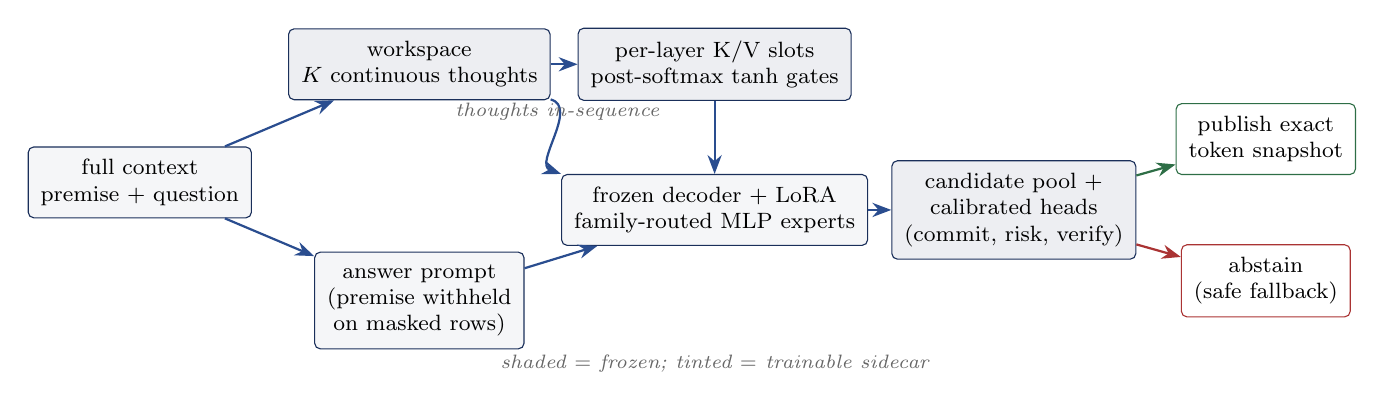
\begin{tikzpicture}[
  font=\footnotesize,
  box/.style={draw=navy, rounded corners=2pt, align=center, inner sep=4.5pt},
  frozen/.style={box, fill=codebg},
  trained/.style={box, fill=navy!8},
  arr/.style={-{Stealth[length=2.4mm]}, thick, draw=accent},
  note/.style={font=\scriptsize\itshape, text=black!60, align=center},
]
\node[frozen] (input) at (0, 0) {full context\\premise $+$ question};
\node[trained] (workspace) at (3.55, 1.5) {workspace\\$K$ continuous thoughts};
\node[frozen] (masked) at (3.55, -1.5) {answer prompt\\(premise withheld\\on masked rows)};
\node[trained] (slots) at (7.3, 1.5) {per-layer K/V slots\\post-softmax $\tanh$ gates};
\node[frozen] (decoder) at (7.3, -0.35) {frozen decoder $+$ LoRA\\family-routed MLP experts};
\node[trained] (heads) at (11.1, -0.35) {candidate pool $+$\\calibrated heads\\(commit, risk, verify)};
\node[box, draw=okgreen] (publish) at (14.3, 0.55) {publish exact\\token snapshot};
\node[box, draw=failred] (abstain) at (14.3, -1.25) {abstain\\(safe fallback)};
\draw[arr] (input) -- (workspace);
\draw[arr] (input) -- (masked);
\draw[arr] (workspace) -- (slots);
\draw[arr] (slots) -- (decoder);
\draw[arr] (workspace) to[out=-15, in=160] node[note, above, pos=0.45]{thoughts in-sequence} (decoder.north west);
\draw[arr] (masked) -- (decoder);
\draw[arr] (decoder) -- (heads);
\draw[arr, draw=okgreen] (heads) -- (publish);
\draw[arr, draw=failred] (heads) -- (abstain);
\node[note] at (7.3, -2.3) {shaded $=$ frozen; tinted $=$ trainable sidecar};
\end{tikzpicture}}%
\caption{The hierarchical latent workspace model. A frozen decoder is
wrapped by three trainable subsystems: a workspace that recirculates the
model's own hidden states as continuous thoughts, a gated per-layer
key--value interface that makes the workspace visible at every depth, and a
calibrated publication layer that either publishes one exact token snapshot
or abstains. On masked rows the answer prompt is physically denied the
premise, so the workspace channel is the only route from evidence to answer; structural necessity is a property of the data, not a regularizer.}
\label{fig:architecture}
\end{figure}

The central research question is:
\begin{list}{}{\leftmargin=1.8em \rightmargin=1.8em}\item\relax
\textbf{\color{navy} Can a root-preserving, variable-depth expert graph
coordinate isolated parallel reasoning and private block revision while
improving verified answer quality at matched active computation?}
\end{list}

The contribution is not simply more experts or more thinking. It is a
three-axis allocation rule: connected expert-graph depth, per-lane recurrent
depth, and macrocycle count, all charged against one declared budget. A general
question may execute only the shared substrate and root for a few recursive
calls. A Python debugging lane may begin with a broad software route,
consolidate what it has learned, descend through Python into debugging and
testing specialists, and halt independently when another update has no measured
value. A multidisciplinary task may activate several routes and several lanes
concurrently. In every case, the shared substrate and root remain structurally
active, their functional contribution is measured through interventions and
anchor tasks, and one budget limits expert-graph depth, private recursive
depth, and macrocycle depth.

\paragraph{Contributions.}
This paper makes four contributions.
\begin{enumerate}[label=\arabic*.]
\item \textbf{An architecture specification} for hierarchical latent
  workspace models: a root-preserving expert graph, a multi-timescale
  isolated-lane workspace with diffusion refinement, and calibrated
  atomic publication, all charged against a single declared compute budget
  (Sections~\ref{sec:design}--\ref{sec:compute}).
\item \textbf{A preregistered evaluation methodology} for architecture
  claims at small scale: gate batteries, margins, and binding decision
  ladders frozen before every run; killer baselines inside every audit;
  semantic graders and split-conformal publication thresholds fitted only on
  generated held-out emissions (Section~\ref{sec:protocol}).
\item \textbf{A complete experimental record} of ten gated experiments on a
  frozen 0.6B substrate (Section~\ref{sec:experiments}). All three proposed
  mechanisms are falsified at this scale, each with a mechanism-level
  diagnosis rather than a bare null: learned routing collapses whenever the
  assignment is learnable; candidate selection is void without measured
  difficulty headroom; and the latent workspace channel carries
  probe-decodable content that generation cannot use, first through
  redundancy and finally under structural necessity (masked-premise transfer
  0.000 on both seeds while a linear probe recovers a third of the withheld
  content). The one surviving positive thread is calibrated selective
  prediction, whose operating points replicate flawlessly and whose
  advantage over free baselines is directionally consistent but below its
  preregistered significance bar.
\item \textbf{A transferable failure taxonomy} for bolt-on reasoning
  structures: every observed pathology (scale-invariant gates, token-id
  aliasing on no-BOS bases, padded harvest surfaces, degenerate calibration
  thresholds, schedule--curriculum aliasing) is named, given a detector, and
  paired with the instrument correction that exposed it
  (Section~\ref{sec:failure}).
\end{enumerate}

\paragraph{Reading guide.}
Sections~\ref{sec:design}--\ref{sec:compute} specify the architecture and
training proposal; Section~\ref{sec:protocol} the protocol;
Section~\ref{sec:experiments} the ten experiments;
Section~\ref{sec:failure} failure modes and decision rules;
Section~\ref{sec:limits} limitations; Section~\ref{sec:prior} related work.
The proposed mechanisms are retained in full as proposal plus negative
evidence; a reader who wants only the outcomes should read
Sections~\ref{sec:study8}, \ref{sec:study9}, \ref{sec:study10}
and~\ref{sec:conclusion}. Artifact provenance is in
Appendix~\ref{app:provenance}.

% ================================================================ 2
\section{Design Specification}
\label{sec:design}

\subsection{Operational commitments and testable assumptions}

The proposal separates mechanisms that define the model from effects that
experiments must establish.

\begin{enumerate}[label=\textbf{I\arabic*.},leftmargin=2.8em]
\item \textbf{Permanent general substrate.} Shared embeddings, attention,
  normalization, and language-output machinery execute in every functional
  stage.
\item \textbf{Always-executed root.} A root/generalist expert cannot be removed
  by graph routing. No fixed mixture percentage is claimed to preserve
  capability; preservation is evaluated behaviorally through preregistered
  non-inferiority and intervention tests.
\item \textbf{Variable-depth graph activation.} The router chooses stop or
  expansion decisions over a fixed candidate expert directed acyclic graph
  (DAG). It does not activate a fixed number of experts or traverse a fixed
  depth.
\item \textbf{Dormancy by default.} Specialists outside the selected
  stage-and-lane subgraph do not execute. They may remain resident in memory,
  but incur no expert forward pass or gradient to their expert parameters for
  that invocation; the router may still receive exploration or regularization
  gradients.
\item \textbf{Private parallel work.} Solver lanes cannot read one another's
  private states. Cross-lane exchange occurs only through identified summaries,
  verification records, and synthesis.
\item \textbf{Shared recursive transition.} The same root-preserving transition
  kernel is reused across lanes, functional modes, and recursive depth.
  Recurrence adds executed computation without allocating depth-specific
  transformer blocks.
\item \textbf{Barrier-mediated global state.} Private lanes update concurrently
  against a frozen global workspace. Only structured summaries and verification
  records cross a synchronization barrier; hidden lane states never enter the
  global workspace directly.
\item \textbf{Atomic publication.} Commitment freezes an exact token-ID
  snapshot. Only those buffered IDs may be appended, after which they are
  causally re-encoded to extend the public key--value cache. Solver canvases
  never publish directly.
\end{enumerate}

These invariants distinguish the proposal from a conventional fixed-width
mixture of experts (MoE), an external tree-search controller, and a multi-agent
workflow.

\subsection{Two hierarchies and model state}

HLWM contains two different structures. The \emph{functional hierarchy}
describes the flow of work:
\begin{center}
framing $\rightarrow$ decomposition $\rightarrow$ solving $\rightarrow$
verification $\rightarrow$ synthesis $\rightarrow$ commitment.
\end{center}
The \emph{parameter graph} is a fixed typed candidate DAG
$\gcand = (\Vcal, \Ecal)$ chosen before a training run:
\begin{center}
root $\rightarrow$ domain $\rightarrow$ capability $\rightarrow$
technology/method $\rightarrow$ operation.
\end{center}

Training learns the expert parameters and a conditional routing policy over its
permitted edges; version one does not add or delete graph edges. The graph need
not be a strict tree: a testing specialist, for example, may have several
admissible parents. Semantic node names are initialization priors and
diagnostic labels, not guarantees about the learned function.

For output block $b$ and macrocycle $r$, the model maintains the state in
Table~\ref{tab:state}.

\begin{table}[htbp]
\caption{Principal state variables. Private state is never appended to
committed context unless synthesis and commitment accept it.}
\label{tab:state}
\centering\small
\begin{tabularx}{\textwidth}{@{}lX@{}}
\toprule
\textbf{Symbol} & \textbf{Meaning} \\
\midrule
$C_b$ & Causally encoded user input and previously committed blocks; fixed while block $b$ is refined. \\
$g_{b,r}$ & Global workspace containing the objective, hard constraints, unresolved dependencies, and verified findings. \\
$\Acal^{m,j}_{b,r,q}$ & Active root-connected expert subgraph for stage $m$, lane $j$, and route window $q$; shared stages omit $j$. \\
$B^{j}_{b,r}$ & Learned brief for solver lane $j$: scope, assumptions, deliverable, dependencies, and failure tests. \\
$w^{j}_{b,r,q}$ & Private slow lane state containing its consolidated plan, unresolved dependencies, and progress after route window $q$. \\
$z^{j}_{b,r,q,s},\, D^{j}_{b,r,q,s}$ & Private fast latent state and categorical canvas at microstep $s$ inside route window $q$. \\
$A^{j}_{b,r}$ & Identified branch summary containing claims, dependencies, route provenance, and uncertainty. \\
$V^{k}_{b,r}$ & Structured verification record for assigned claims or candidates. \\
$Y_{b,r}$ & Separately refined private synthesis block; the only block eligible for publication. \\
\bottomrule
\end{tabularx}
\end{table}

% ================================================================ 3
\section{Dynamic Root-Preserving Expert Graph}
\label{sec:graph}

\subsection{Stage-progressive, budgeted graph traversal}

Let the fixed candidate DAG be $\gcand = (\Vcal, \Ecal)$ with root node $v_0$.
Immediately before stage $m$, the dispatcher observes every result that is
legitimately available at that point:
\begin{equation*}
\xi^{m,j}_{b,r} = \bigl(C_b,\; g_{b,r},\; e_m,\; e_j,\; \text{stage inputs},\;
\text{verified history},\; \text{remaining budget}\bigr),
\end{equation*}
where $e_m$ and $e_j$ are stage and lane embeddings. The router predicts a
logit $\ell_v(\xi)$ for every specialist reachable under the current ancestry
mask. A horizon head also predicts ordered continuation logits
$r_{m,j,1:N^m_{\max}}(\xi)$; accepting increment $n$ requires accepting every
earlier increment, so the requested fast-update cap $N^{m,j}_{\mathrm{cap}}$ is
a prefix rather than an unconstrained integer. The stage schedule
deterministically expands that cap into $N^{m,j}_\Phi$ shared-kernel
invocations, including every required private consolidation. For route $j$ in
stage $m$, binary execution gates and this complete scheduled count satisfy
\begin{align}
a^{m,j}_{v_0} &= 1, \\
a^{m,j}_{v} &\le \sum_{p \in \op{Pa}(v)} a^{m,j}_{p} \quad (v \ne v_0),
\end{align}
\begin{equation}
\EC\bigl(\Acal^{m,j}, N^{m,j}_\Phi\bigr) = c_{\mathrm{route}}
+ c^{m,j}_{\mathrm{aux}}
+ N^{m,j}_\Phi \Biggl( c_{\mathrm{shared}} + c_0
+ \sum_{v \in \Acal^{m,j} \setminus \{v_0\}} c_v \Biggr).
\end{equation}
Here $\EC$ denotes execution cost. Every active specialist has a recursively
active path to the root, activating no child is the specialist stop action, and
repeated use of an expert is charged repeatedly. $N^{m,j}_\Phi$ includes fast
transitions and scheduled private consolidations; $c^{m,j}_{\mathrm{aux}}$
covers declared heads, routing, summary extraction, and other non-kernel work
assigned to that reservation. Version one learns the gates and expert
parameters, not the candidate topology.

One atomic block ledger first escrows a private causal-fallback reserve and
exposes only the remaining balance to macrocycles. Before any parallel
interval, every unfinished lane submits route scores and a requested
fast-update cap. A joint allocator chooses
$\{(\Acal^{m,j}, N^{m,j}_{\mathrm{cap}})\}_{j \in \Jcal_q}$ and expands each
cap into its complete scheduled count $N^{m,j}_\Phi$ under
\begin{equation}
\sum_{j \in \Jcal_q} \EC\bigl(\Acal^{m,j}, N^{m,j}_\Phi\bigr)
+ B_{\mathrm{downstream}} \le B_{\mathrm{remain}},
\label{eq:budget}
\end{equation}
where $B_{\mathrm{downstream}}$ reserves declared minimum cost for routing and
control, branch summaries, verification, the global slow update, synthesis, the
root-preserving commitment transition, risk and expected-value-of-information
(EVI) scoring, and causal cache extension. The fallback is excluded here
because one fallback escrow, covering control, causal generation,
commitment-state construction, risk scoring, and possible cache extension, was
created exactly once at block-ledger initialization; $B_{\mathrm{remain}}$ is
the spendable balance after that escrow. Every learned forward pass and every
non-negligible routing, checking, or control operation must draw from a named
reservation before executing and atomically settle its measured cost
afterward. Constant-time ledger comparisons are not learned model computation.
If the minimum per-lane reservations are infeasible, the dispatcher reduces the
lane set before execution; no lane may spend another lane's reservation
speculatively. Consequently, simultaneous initial routes, consolidations,
refreshes, scoring, and publication cannot exceed the block budget.

During training, each discrete node bid uses a straight-through Binary-Concrete
estimator. The horizon request uses relaxed prefix gates, so its previously
implicit estimator is explicit. For independent
$u_v, u_n \sim \op{Uniform}(0,1)$, let $g(u) = \log u - \log(1-u)$ and define
\begin{align}
\widetilde{a}_v &= \sigma\!\left( \frac{\ell_v + g(u_v)}{\tau_a} \right), \\
\widetilde{c}_{m,j,n} = \prod_{i=1}^{n}
  \sigma\!\left( \frac{r_{m,j,i} + g(u_i)}{\tau_N} \right),
&\qquad
\widetilde{N}^{m,j}_{\mathrm{cap}} = \sum_{n=1}^{N^m_{\max}}
  \widetilde{c}_{m,j,n}, \\
(\mathbf{a}^{\mathrm{hard}}, \mathbf{N}^{\mathrm{hard}}_{\mathrm{cap}})
  &= \Pi_{B_{\mathrm{remain}}}
  (\widetilde{\mathbf{a}}, \widetilde{\mathbf{c}};\, \gcand), \\
\mathbf{a}^{\mathrm{ST}} &= \stopgrad(\mathbf{a}^{\mathrm{hard}}
  - \widetilde{\mathbf{a}}) + \widetilde{\mathbf{a}}, \\
\mathbf{N}^{\mathrm{ST}}_{\mathrm{cap}} &=
  \stopgrad(\mathbf{N}^{\mathrm{hard}}_{\mathrm{cap}}
  - \widetilde{\mathbf{N}}_{\mathrm{cap}}) + \widetilde{\mathbf{N}}_{\mathrm{cap}}.
\end{align}
The deterministic projection $\Pi_{B_{\mathrm{remain}}}$ first reserves the
minimum complete schedule for every admitted lane, then adds feasible
transition calls and nodes, together with missing ancestors, in marginal
score-to-execution-cost order while enforcing
equation~\eqref{eq:budget}. A call increment is admitted only after its prefix
and any required consolidation call; stable lane and node identifiers break
ties. The forward pass executes only the hard route and hard horizon, so an
inactive expert receives neither an expert forward pass nor an
expert-parameter gradient. The relaxed terms supply biased, low-variance
router and horizon gradients; score-function estimators are required controls.
At inference, noise is removed and the same joint projection is applied to node
and ordered continuation logits. This is a declared version-one estimator, not
a claim that it is optimal~\cite{louizos2018}.

Framing is routed from committed context and the previous frame; decomposition
is routed after the new frame exists; solver paths are conditioned on learned
briefs; verifier paths are conditioned on resulting claims; and synthesis is
routed after verification findings exist. Within a recurrent stage, a route is
fixed for one bounded window of at most $K$ fast updates. At the next boundary,
each unfinished lane may form a refresh bid from only its own consolidated
private state; the joint allocator arbitrates all bids against the shared
ledger. This preserves state isolation and coherent specialist work inside a
window while allowing broad early routes to descend toward newly discovered
specialist operations without exceeding the macrocycle budget.

\emph{In plain terms:} the model bids for computation the way a project bids
against a budget. Each lane proposes how deep it wants to specialize and how
many refinement steps it wants; a single ledger admits what fits, always
keeping enough in reserve to verify, synthesize, and publish safely.

This produces a distribution of active computation rather than one advertised
number. For one stage and lane,
\begin{equation}
P^{m,j}_{\mathrm{active}}(x) = P_{\mathrm{trunk}} + P_0
+ \sum_{v \in \Acal^{m,j}(x) \setminus \{v_0\}} P_v .
\end{equation}
A proper report gives minimum, mean, 95th percentile, maximum, and per-stage
distributions of active parameters and FLOPs. An eight-billion-active label is
not an architectural constant of HLWM.

\subsection{Always-executed root and behavioral retention}
\label{sec:root}

Simply executing the root does not establish that it contributes useful
general capability. Conversely, a large residual coefficient does not measure
retained language ability: later layers, vector cancellation, and the shared
trunk all intervene. HLWM therefore separates \emph{structural root presence}
from \emph{behavioral preservation}. For expert $v$, let $\op{RMS}$ denote
root-mean-square magnitude over hidden dimensions and define a normalized
output
\begin{equation}
\widehat{E}_v(h) = \frac{E_v(h)}{\op{RMS}(E_v(h)) + \eps_{\mathrm{num}}} .
\end{equation}
Let $T_\theta$ be the permanent shared substrate, let
$\gamma_0 = \op{softplus}(\eta_0)$ and $\gamma_s = \op{softplus}(\eta_s)$ be
learned layerwise scales that do not depend on the task route, and let
$s(x, m, j) = \op{softplus}(a_s)$ be a nonnegative route-conditioned specialist
strength. A connected graph is not executed as a flat weighted sum. It performs
one topological downward sweep followed by a reverse-topological upward sweep.
With $\alpha_{pv}$ normalized over the active parents of $v$, $\beta_{vc}$
assigning each child message across its active parents, and $\op{LN}$ denoting
layer normalization, define
\begin{align}
h_{\mathrm{shared}} = T_\theta(h), &\qquad r_0 = \widehat{E}_0(h_{\mathrm{shared}}), \\
r_v = \widehat{E}_v\!\Biggl( \op{LN}\Biggl[ h_{\mathrm{shared}} + \gamma_0 W_0 r_0
  + \sum_{p \in \op{Pa}_{\Acal}(v)} \alpha_{pv} U_{pv} r_p \Biggr] \Biggr),
  &\qquad v \in \Acal \setminus \{v_0\}, \\
u_v = r_v + \sum_{c \in \op{Ch}_{\Acal}(v)} \beta_{vc} R_{vc} u_c,
  &\qquad v \in \Acal \quad \text{in reverse order}, \\
h' = h_{\mathrm{shared}} + \gamma_0 W_0 r_0 + s(x,m,j)\, \gamma_s W_s (u_0 - r_0). &
\label{eq:hupdate}
\end{align}
For a DAG, $\sum_{p \in \op{Pa}_{\Acal}(c)} \beta_{pc} = 1$ prevents a multiply
parented child from being counted once per parent. If no specialist is active,
$u_0 = r_0$ and the specialist residual is exactly zero. Active siblings at the
same graph depth execute concurrently; only ancestor--descendant dependencies
impose sequential graph depth. Thus adding a deeper node changes both the
context it receives and the evidence returned toward the root, rather than
merely adding another flat expert output.

The root has no router-controlled gate: its message conditions every active
specialist, remains an explicit residual in the final update, and is recomputed
on every recursive invocation. Specialist strength may become large on narrow
work, but no scalar in equation~\eqref{eq:hupdate} is interpreted as a
percentage of intelligence, fluency, or reasoning. Layerwise root and
specialist residual norms, edge-message norms, directional alignment, and
ablation effects are reported as diagnostics. Held-out behavior, rather than
$\gamma_0$, determines whether the root remains functionally useful.

Functional preservation is defined on preregistered anchor families
$\{\Dcal_k\}_{k=1}^{K}$ covering language modeling, instruction adherence,
discourse coherence, global constraints, and other claimed general
capabilities. Let $p_{\mathrm{ref}}$ be a frozen competent reference,
$p_{\mathrm{root}}$ the current shared-plus-root path with specialists
disabled, and $p_{\mathrm{full}}$ the routed model. For a loss $\Lcal_k$ whose
lower value is better, define
\begin{align}
\Delta^{\mathrm{root}}_k &= \Lcal_k(p_{\mathrm{root}}; \Dcal_k)
  - \Lcal_k(p_{\mathrm{ref}}; \Dcal_k), \\
\Delta^{\mathrm{route}}_k &= \Lcal_k(p_{\mathrm{full}}; \Dcal_k)
  - \Lcal_k(p_{\mathrm{root}}; \Dcal_k).
\label{eq:routegap}
\end{align}
Training targets the constrained problem
\begin{equation}
\min_\theta\; \Lcal_{\mathrm{task}} + \lambda_C\, \E[\op{Cost}(x)]
\quad \text{subject to} \quad
\Delta^{\mathrm{root}}_k \le \eps^{\mathrm{root}}_k, \;\;
\Delta^{\mathrm{route}}_k \le \eps^{\mathrm{route}}_k \quad \forall k.
\label{eq:constrained}
\end{equation}
The tolerances $\eps_k$ must be declared before final evaluation and justified
by measurement uncertainty or application requirements. They are not universal
constants. Dual optimization or an equivalent Lagrangian can optimize toward
the constraints; held-out confidence bounds determine whether the constraints
are actually satisfied. Counterfactual root ablation, specialist masking, and
held-out anchor results determine whether the root is functionally useful;
architectural presence alone is insufficient. Specialist value on domain $d$
is measured by the counterfactual gain
\begin{equation}
G_{\mathrm{spec}}(d) = \Rcal_d(p_{\mathrm{root}}) - \Rcal_d(p_{\mathrm{full}}),
\end{equation}
for a preregistered risk $\Rcal_d$ whose lower value is better. This tests
whether specialists add capability rather than merely receive high routing
scores.

Adaptive halting exposes several possible readout depths, so terminal-only
retention is insufficient. For halt-eligible readouts $q \in \Qcal_{\mathrm{halt}}$,
define both the root-only and routed gaps
\begin{align}
\Delta^{\mathrm{root}}_{k,q} &= \Lcal_k\bigl(p^{(q)}_{\mathrm{root}}; \Dcal_k\bigr)
  - \Lcal_k(p_{\mathrm{ref}}; \Dcal_k), \\
\Delta^{\mathrm{route}}_{k,q} &= \Lcal_k\bigl(p^{(q)}_{\mathrm{full}}; \Dcal_k\bigr)
  - \Lcal_k\bigl(p^{(q)}_{\mathrm{root}}; \Dcal_k\bigr),
\end{align}
\begin{equation}
\max_{q \in \Qcal_{\mathrm{halt}}} \Delta^{\mathrm{root}}_{k,q}
  \le \eps^{\mathrm{root}}_k,
\qquad
\max_{q \in \Qcal_{\mathrm{halt}}} \Delta^{\mathrm{route}}_{k,q}
  \le \eps^{\mathrm{route}}_k .
\label{eq:haltgaps}
\end{equation}
Training may sample readout depths to estimate these constraints, but final
evaluation tests both gaps at every declared halt-eligible depth. Root
execution at every recursive call is structural; retained competence of both
the root-only and routed paths at those calls remains a behavioral claim.

\subsection{Illustrative activation, not a handwritten schedule}

Figure~\ref{fig:activation} shows the intended qualitative behavior. A general
prompt stops at the root. A Python debugging request expands a relevant
connected subgraph; unrelated domains remain dormant. The dispatcher learns
this behavior from outcomes and budget pressure. Training records do not
prescribe hand-authored phase weights.

\begin{figure}[htbp]
\centering
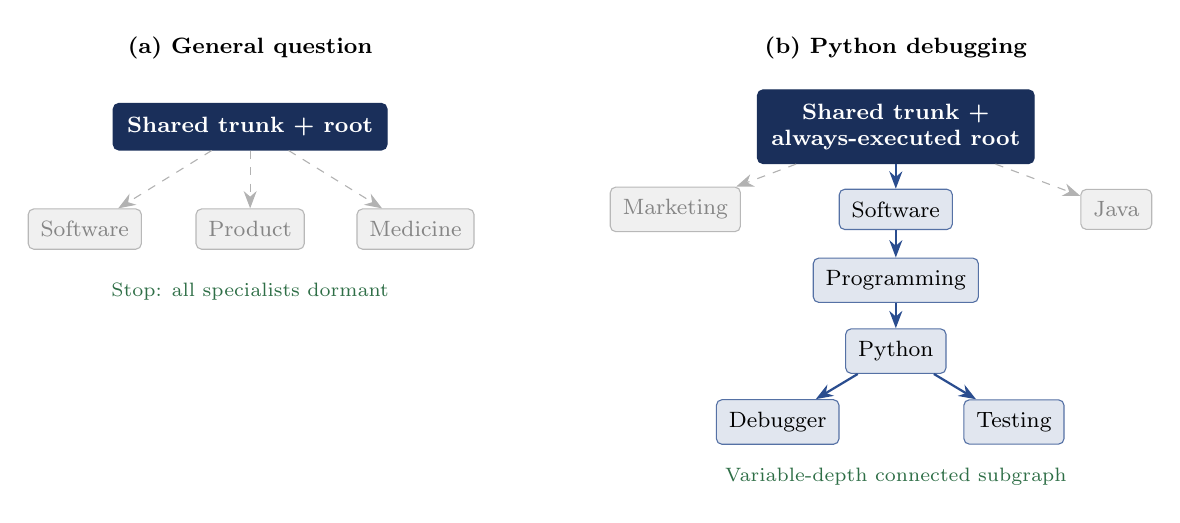
\begin{tikzpicture}[
  font=\small,
  rootnode/.style={draw=navy, fill=navy, text=white, rounded corners=2pt,
    inner sep=5pt, align=center, font=\footnotesize\bfseries},
  activenode/.style={draw=accent!80, fill=accent!14, rounded corners=2pt,
    inner sep=4.5pt, align=center, font=\footnotesize},
  dormantnode/.style={draw=black!28, fill=black!6, text=black!48,
    rounded corners=2pt, inner sep=4.5pt, align=center, font=\footnotesize},
  activeedge/.style={-{Stealth[length=2.2mm]}, thick, accent},
  dormantedge/.style={-{Stealth[length=2.2mm]}, black!30, dashed},
  panellabel/.style={font=\footnotesize\bfseries},
  note/.style={font=\scriptsize, text=okgreen}
]
% ---------------- panel (a): general question ----------------
\begin{scope}[xshift=0cm]
  \node[panellabel] at (0,2.4) {(a) General question};
  \node[rootnode] (rootA) at (0,1.4) {Shared trunk + root};
  \node[dormantnode] (sw) at (-2.1,0.1) {Software};
  \node[dormantnode] (pr) at (0,0.1) {Product};
  \node[dormantnode] (me) at (2.1,0.1) {Medicine};
  \draw[dormantedge] (rootA) -- (sw);
  \draw[dormantedge] (rootA) -- (pr);
  \draw[dormantedge] (rootA) -- (me);
  \node[note] at (0,-0.7) {Stop: all specialists dormant};
\end{scope}
% ---------------- panel (b): Python debugging ----------------
\begin{scope}[xshift=8.2cm]
  \node[panellabel] at (0,2.4) {(b) Python debugging};
  \node[rootnode] (rootB) at (0,1.4) {Shared trunk +\\always-executed root};
  \node[dormantnode] (mk) at (-2.8,0.35) {Marketing};
  \node[activenode] (sf) at (0,0.35) {Software};
  \node[dormantnode] (jv) at (2.8,0.35) {Java};
  \node[activenode] (pg) at (0,-0.55) {Programming};
  \node[activenode] (py) at (0,-1.45) {Python};
  \node[activenode] (db) at (-1.5,-2.35) {Debugger};
  \node[activenode] (ts) at (1.5,-2.35) {Testing};
  \draw[dormantedge] (rootB) -- (mk);
  \draw[activeedge] (rootB) -- (sf);
  \draw[dormantedge] (rootB) -- (jv);
  \draw[activeedge] (sf) -- (pg);
  \draw[activeedge] (pg) -- (py);
  \draw[activeedge] (py) -- (db);
  \draw[activeedge] (py) -- (ts);
  \node[note] at (0,-3.05) {Variable-depth connected subgraph};
\end{scope}
\end{tikzpicture}
\caption{Task-dependent activation of the expert graph. Shaded nodes execute;
gray nodes do not. The example illustrates expected behavior, not fixed
semantic routes or manually supplied weights.}
\label{fig:activation}
\end{figure}
% ================================================================ 4
\section{Parallel Latent Workspace}
\label{sec:workspace}

\subsection{Adaptive lanes, distinct briefs, and isolation}

The architecture provides at most $J_{\max}$ solver lanes, but the dispatcher
activates a task-dependent subset $\Jcal_{b,r}$. A simple prompt may use one
root-only lane. A difficult debugging task may use implementation, test, and
adversarial lanes. Joint decomposition first proposes a candidate lane set and
its briefs, then one allocator admits a feasible subset and all initial
schedules together:
\begin{align}
\Bigl( \widetilde{\Jcal},\, \{B^j\}_{j \in \widetilde{\Jcal}} \Bigr)
  &= \op{BriefHead}\bigl( C,\, g,\, \{e_j\},\, B_{\mathrm{remain}} \bigr), \\
\Bigl( \Jcal,\, \{(\Acal^{m,j}_0, N^{m,j}_{\mathrm{cap}})\}_{j \in \Jcal} \Bigr)
  &= \op{JointAllocate}\Bigl( \{\op{RouteBid}(C, g, B^j)\}_{j \in \widetilde{\Jcal}},\,
  B_{\mathrm{remain}} \Bigr), \qquad \Jcal \subseteq \widetilde{\Jcal}.
\end{align}
Each brief specifies scope, allowed assumptions, expected deliverables,
dependencies, and rejection tests. Branches may be complementary, competitive,
or adversarial. Diversity is evaluated from verified informational contribution
rather than route names or raw token disagreement. Let $\Rcal(x)$ be the finite
set of evaluator-defined requirements for task $x$, let $C_j$ be the atomic
claims recorded by lane $j$, and let $v(c) \in \{0,1\}$ be an executable or
independently adjudicated correctness label. With
$C^+_j = \{c \in C_j : v(c) = 1\}$, define
\begin{align}
\op{Cov}(x) &= \frac{1}{|\Rcal(x)|} \sum_{r \in \Rcal(x)}
  \mathbf{1}\Bigl[ \exists j,\, c \in C^+_j : c \models r \Bigr], \\
\op{Red}(x) &= \frac{2}{J(J-1)} \sum_{i < j}
  \frac{\bigl| C^+_i \cap_{\sim} C^+_j \bigr|}{\bigl| C^+_i \cup_{\sim} C^+_j \bigr|}, \\
M_j(x) &= U(Y_{\mathrm{all}}, x) - U(Y_{\setminus j}, x).
\label{eq:marginal}
\end{align}
Here $\sim$ is a preregistered semantic-equivalence rule. Redundancy is
reported only for $J \ge 2$ and nonempty unions. To estimate $M_j$, synthesis
is rerun without summary $A^j$ while its route, compute budget, and sampling
randomness are held fixed. Multiple lanes count as useful only when they
improve verified coverage or utility without increasing verified error;
disagreement alone is not productive diversity.

During solving, lane $j$ may attend to $C$, $g$, $B^j$, $w^j$, $z^j$, and
$D^j$, but not to another lane's private state. The public inputs are
read-only during the solver interval, and attention masks enforce
\begin{equation}
\frac{\partial H^j_{q,s}}{\partial w^i_{q'}} = 0,
\qquad
\frac{\partial H^j_{q,s}}{\partial z^i_{q',s'}} = 0,
\qquad
\frac{\partial H^j_{q,s}}{\partial D^i_{q',s'}} = 0
\quad (i \ne j)
\end{equation}
within that interval. A synchronization barrier materializes every identified
summary before verification or synthesis can read it. Shared parameters,
common context, and related briefs can still correlate outputs;
\emph{state-isolated} is an information-flow claim, not statistical
independence. After solving, the structured summary
\begin{equation}
A^j = \op{SummaryHead}\bigl( B^j, w^j, z^j, D^j, \Acal^{\mathrm{solve},j}_{0:Q_j} \bigr)
\end{equation}
records atomic claims, requirement links, dependencies, uncertainty, and route
provenance for downstream verification and synthesis. This boundary preserves
alternatives long enough to be useful without turning the model into
communicating agents.

Because the transition parameters are shared across lanes, collapse is an
explicit risk. Lanes are differentiated by jointly generated briefs, lane
embeddings, independently keyed initialization noise, and potentially
different routes. Hidden-state repulsion is not treated as evidence of useful
diversity because it can reward different errors. The accepted criteria remain
verified coverage, verified redundancy, and fixed-randomness marginal
synthesis utility from equation~\eqref{eq:marginal}.

\subsection{Root-preserving multi-rate recurrence}
\label{sec:recurrence}

The same private recurrence is used for stages
$m \in \mathcal{M}_{\mathrm{priv}} = \{\text{solve}, \text{verify},
\text{synthesize}\}$. Its stage input $B^{m,j}$ is respectively a solver
brief, a claim assignment with rejection tests, or a verified integration
contract; synthesis normally uses one lane, while solving and verification may
use several. Every newly activated private lane receives a slow state, fast
state, categorical canvas, and empty self-conditioning state. For readability,
the following equations suppress $m$ on recurrent states, but initialization,
mode embeddings, output heads, validity boundaries, utilities, and maximum
horizons remain stage-conditioned:
\begin{align}
w^j_0 &= \op{Init}_w\bigl( C_b, g_{b,r}, B^{m,j}, e_m, e_j \bigr), \\
z^j_{0,0} &= \op{Init}_z\bigl( C_b, g_{b,r}, B^{m,j}, w^j_0, e_m, e_j \bigr)
  + \sigma_z \epsilon_j, \qquad \epsilon_j \sim \mathcal{N}(0, I), \\
D^j_{0,0} \sim \op{Cat}(\nu)^{L_j}, &\qquad S^j_{0,0} = 0 .
\end{align}
All recurrent roles reuse one transition kernel $\Phi_\theta$ under
functional-mode, stage, lane, timescale, and depth embeddings. Small
mode-specific projections map state types to and from its common width; no
transformer block is allocated to a particular lane or recursive step. At fast
microstep $s$ of route window $q$, lane $j$ forms
\begin{align}
\chi^j_{q,s} &= \op{Pack}\bigl( C_b, g_{b,r}, B^{m,j}, w^j_q, z^j_{q,s},
  D^j_{q,s}, S^j_{q,s}, e_m, e_j, e_q, e_s \bigr), \\
H^j_{q,s} &= \Phi_\theta\Bigl( \chi^j_{q,s};\; \Acal^{m,j}_q \Bigr).
\end{align}
Every invocation of $\Phi_\theta$ applies the permanent shared substrate and
the root-preserving graph operator in equation~\eqref{eq:hupdate}; only
specialists in $\Acal^{m,j}_q$ are conditional. Reusing $\Phi_\theta$
increases executed depth without increasing stored depth-specific parameters.
This weight tying is a testable efficiency choice, not a guarantee of improved
reasoning.

Flatten $(q, s)$ to update index $n = qK + s$. A declared stage schedule
$t_{q,s} = \tau_m(n)$ maps each executed update to its reverse
categorical-diffusion timestep; targeted re-noising is represented by an
explicit per-position timestep mask rather than an undefined reset of
$t_{q,s}$.

The fast head updates the private latent and diffusion states and predicts the
externally testable value of another update:
\begin{align}
\bigl( \overline{z}^j_{q,s+1},\, u^j_{q,s},\, P^j_{q,s},\, \eta^j_{q,s},\,
  \widehat{d}^{\,j}_{q,s} \bigr) &= \op{FastHead}\bigl( H^j_{q,s} \bigr), \\
z^j_{q,s+1} &= \bigl( 1 - \sigma(u^j_{q,s}) \bigr) \odot z^j_{q,s}
  + \sigma(u^j_{q,s}) \odot \overline{z}^j_{q,s+1}, \\
\overline{D}^j_{q,s+1} &\sim \op{ReverseCat}\bigl( D^j_{q,s}, P^j_{q,s},
  t_{q,s} \bigr), \\
D^j_{q,s+1,i} &= \op{Select}\bigl( m^{\mathrm{sample}}_{q,s,i},\,
  \overline{D}^j_{q,s+1,i},\, D^j_{q,s,i} \bigr), \\
S^j_{q,s+1} &= \stopgrad\bigl( P^j_{q,s} E_{\mathrm{tok}} \bigr).
\label{eq:selfcond}
\end{align}
After at most $K$ fast updates, each unfinished lane privately consolidates
what it has learned:
\begin{align}
\overline{H}^j_q &= \op{Pool}\bigl\{ H^j_{q,s} : 0 \le s < K \bigr\}, \\
\bigl( \overline{w}^j_{q+1},\, \kappa^j_q \bigr) &=
  \op{SlowHead}\Bigl( \Phi_\theta\bigl( \op{Pack}( C_b, g_{b,r}, B^{m,j},
  w^j_q, \overline{H}^j_q, e_m, e_{\mathrm{consolidate}} );\,
  \Acal^{m,j}_q \bigr) \Bigr), \\
w^j_{q+1} &= \bigl( 1 - \sigma(\kappa^j_q) \bigr) \odot w^j_q
  + \sigma(\kappa^j_q) \odot \overline{w}^j_{q+1} .
\end{align}
This slow update remains private to lane $j$. It does not average lane states
or write into the global workspace.

At a window boundary, every unfinished lane forms a refresh bid from public
read-only state and only its own consolidated state. Writing
$\chi^{j+}_q = \bigl( C_b, g, B^{m,j}, w^j_{q+1}, z^j_{q,K}, D^j_{q,K} \bigr)$
for lane $j$'s post-consolidation observation, the dispatcher then solves one
joint allocation:
\begin{equation}
\begin{aligned}
\{(\Acal^{m,j}_{q+1},\, n^{m,j}_{q+1})\}_{j \in \Jcal_q}
={}& \arg\max_{\{(\Acal^j, n^j)\} \in \Fcal_{\mathrm{joint}}}
\sum_{j \in \Jcal_q} \Biggl[\,
\sum_{v \in \Acal^j} \ell_v\bigl( \chi^{j+}_q \bigr) \\
&\quad + \sum_{i=1}^{n^j} r_{m,j,i}\bigl( \chi^{j+}_q \bigr)
- \lambda_{\mathrm{switch}} \op{Cost}\bigl( \Acal^j \,\triangle\,
  \Acal^{m,j}_q \bigr) \Biggr],
\end{aligned}
\label{eq:jointrefresh}
\end{equation}
where $\Fcal_{\mathrm{joint}}$ contains collections of root-connected routes
and prefix horizons satisfying equation~\eqref{eq:budget}, and $\triangle$ is
symmetric difference. The horizon term makes the selected $n^j$ operational
rather than a free argmax variable. The implementation uses the projection and
estimator of the preceding section. Arbitration receives bids, costs, and
route identifiers, not writable lane states; its decisions are returned
simultaneously. The switch cost discourages route thrashing but permits a
broad route to deepen, fork, or change when private progress reveals a more
useful specialist. Refresh never disables the shared substrate or root and
never allows one lane to read another lane's private state.

A within-stage route refresh does not reset $w^j$, $z^j$, or supported canvas
positions, because the brief and private computation remain the same. A new
brief, lane, macrocycle, committed block, or abstention performs a full
private-state reset. A verification-directed retry may export an identified
retry record containing only supported claims, supported token IDs with
positions, conflicts, and provenance. The next macrocycle initializes a fresh
canvas from that record, draws every disputed position from the declared noise
distribution, and clears all self-conditioning. No hidden solver, verifier,
latent, or slow state crosses a macrocycle boundary.

\subsection{Adaptive private depth}
\label{sec:halting}

Private halting allocates compute; it cannot authorize publication. For stage
$m$, flatten $(q, s)$ into $n \in \{1, \dots, N^{m,j}_{\max}\}$. A training
episode may supervise only some depths. Define the eligible halt set
$\Hcal_{m,j}$ to contain depths with a grounded stage-specific output target;
every nonterminal member must additionally have a paired next-update target.
If $\Hcal_{m,j}$ is empty, that episode contributes no halt loss. With
$n^\dagger = \max \Hcal_{m,j}$, the halt logit in
equation~\eqref{eq:selfcond}'s head defines
\begin{align}
h^{m,j}_n &=
\begin{cases}
\sigma(\eta^{m,j}_n), & n \in \Hcal_{m,j},\; n < n^\dagger, \\
1, & n = n^\dagger, \\
0, & n \notin \Hcal_{m,j},
\end{cases} \\
\rho^{m,j}_n = \prod_{\substack{i \in \Hcal_{m,j} \\ i < n}}
  \bigl( 1 - h^{m,j}_i \bigr),
&\qquad
\pi^{m,j}_n = \rho^{m,j}_n\, h^{m,j}_n .
\end{align}
Thus probability mass cannot disappear into an unlabeled early depth. Solver
utility measures the lane's verified brief contribution; verifier utility
measures claim-error discrimination or checker agreement; synthesis utility
measures verified integrated-task quality. In every case the stage-conditioned
utility $U_{m,j}$ is externally scored. For $n < n^\dagger$, paired
continuation gives
\begin{equation}
d_{m,j,n} = U_{m,j}(o_{m,j,n+1}) - U_{m,j}(o_{m,j,n})
  - \lambda_C \bigl( C_{m,j,n+1} - C_{m,j,n} \bigr).
\end{equation}
Let $\Hcal^-_{m,j} = \Hcal_{m,j} \setminus \{n^\dagger\}$. The eligible
halting objective is
\begin{equation}
\begin{aligned}
\Lcal_{\mathrm{halt}} ={}& \sum_{m,j} \frac{1}{|\Hcal_{m,j}| + \eps_{\mathrm{num}}}
  \sum_{n \in \Hcal_{m,j}} \pi^{m,j}_n
  \Bigl( \ell^{\mathrm{out}}_{m,j,n} + \lambda_{\mathrm{step}} C_{m,j,\le n} \Bigr) \\
&+ \sum_{m,j} \frac{\lambda_{\mathrm{gain}}}{|\Hcal^-_{m,j}| + \eps_{\mathrm{num}}}
  \sum_{n \in \Hcal^-_{m,j}} \rho^{m,j}_n
  \op{Huber}\bigl( \widehat{d}_{m,j,n},\, d_{m,j,n} \bigr),
\end{aligned}
\end{equation}
where empty sums are zero. The compute penalty is applied only at eligible,
grounded outputs; sparse labels therefore cannot teach an unpenalized
immediate exit.

The next-update bound must remain valid after repeatedly inspecting depths and
stopping adaptively. On a disjoint stage-stratified calibration split, run the
frozen routing and halting policy and let $\Ical^m_e$ contain every
boundary-valid lane--depth pair that the policy could inspect in calibration
episode $e$. Define one episode-level maximum residual
\begin{equation}
R^m_e = \max_{(j,n) \in \Ical^m_e}
  \Bigl( d_{e,m,j,n} - \widehat{d}_{e,m,j,n} \Bigr),
\end{equation}
with empty sets handled by a predeclared omission or pooling rule, and let
$q^m_{1-\alpha_h}$ be the finite-sample conformal quantile of the $R^m_e$
values. Then every inspected depth in an exchangeable test episode shares the
simultaneous upper confidence bound (UCB)
\begin{equation}
\op{UCB}_{1-\alpha_h}\bigl( \widehat{d}_{m,j,n} \bigr)
= \widehat{d}_{m,j,n} + q^m_{1-\alpha_h} .
\label{eq:haltucb}
\end{equation}
The strata, any predeclared low-sample pooling, $\alpha_h$, and the
cumulative-mass threshold are selected before final evaluation; quantiles and
the policy are frozen. Episode-level simultaneous coverage and its stage/depth
breakdown are both reported. At inference, eligibility is the declared set of
boundary-valid readouts rather than label availability. The allocator admits a
complete schedule only when
$N^{m}_{\min} \le N^{m,j}_{\mathrm{cap}} \le N^{m}_{\max}$ and its final
readout is boundary-valid. Lane $(m,j)$ halts at the first $n \ge N^m_{\min}$
for which cumulative halt mass exceeds the frozen threshold, the boundary is
valid, and equation~\eqref{eq:haltucb} is nonpositive. If that event never
occurs, execution ends at $N^{m,j}_{\mathrm{cap}}$ as an explicit \emph{budget
cap}, not as a calibrated halt. Halted and budget-capped lanes both break their
update loops and become compacted masked no-ops; their termination reasons are
logged separately. Categorical sampler stopping, private recursive halting,
budget capping, macrocycle continuation, and public commitment are distinct
decisions and are evaluated separately.

\subsection{Synchronization and global recurrence}

Solver lanes execute without cross-lane communication until every lane halts or
reaches its cap. A solver barrier materializes identified summaries $\{A^j\}$
simultaneously. Claim-assigned verifier lanes then run the same root-preserving
recurrent kernel in parallel under state-isolating masks. A verifier barrier
materializes $\{V^k\}$. Only after this second barrier may the global workspace
change.

Let $R_r = \op{VerifiedSetEncoder}(\{A^j\}, \{V^k\})$ be permutation-invariant
over identified records and mask unsupported branch content. The shared
transition performs
\begin{align}
\bigl( \overline{g}_{b,r+1},\, \alpha_r \bigr) &=
  \op{GlobalHead}\Bigl( \Phi_\theta\bigl( \op{Pack}( C_b, g_{b,r}, R_r,
  e_{\mathrm{global}} );\; \Acal^{\mathrm{global}}_r \bigr) \Bigr), \\
g_{b,r+1} &= \bigl( 1 - \sigma(\alpha_r) \bigr) \odot g_{b,r}
  + \sigma(\alpha_r) \odot \overline{g}_{b,r+1} .
\end{align}
Thus fast states update at every private microstep, private slow states update
at route-window boundaries, and the global workspace updates only after
verified fan-in. The new global state may be broadcast into the next
macrocycle, where briefs and routes are redispatched. Shared parameters do not
imply shared writable state.

The tied transition accumulates gradients from every supervised application.
Small experiments use full backpropagation through the declared fast and slow
horizons. Scaled experiments declare fast horizon $H_f$ and slow horizon
$H_s$, detach only at those boundaries, and never propagate across a committed
public-block boundary. The primary model permits synthesis gradients to pass
through structured summaries into their producing lanes within the active
horizon. A stop-gradient summary barrier is a required ablation because
end-to-end credit may either improve coordination or collapse lane diversity.

\subsection{Six functional stages}

One root-preserving transition kernel is reused under mode embeddings and
information-flow masks. Stages are functions of one parameter system, not six
independent transformer stacks.

Framing, decomposition, and the barrier-mediated global update invoke the same
$\Phi_\theta$ with stage-specific projections but no private categorical
canvas. Solver, verifier, and synthesis stages use the fully specified private
recurrence of Section~\ref{sec:recurrence}; their inputs and utility targets
differ, not their parameter system. The functional flow is shown in
Figure~\ref{fig:macrocycle}, and the stages are summarized in
Table~\ref{tab:stages}.

\begin{figure}[htbp]
\centering
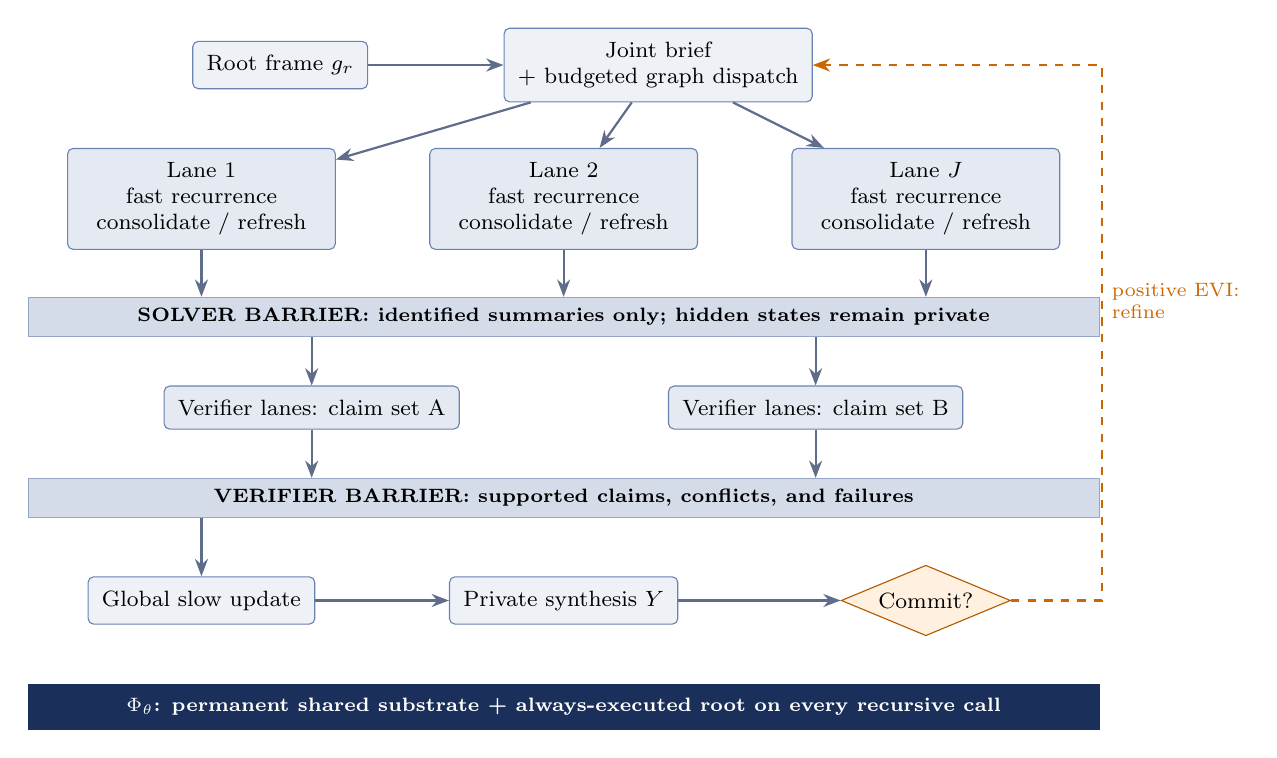
\begin{tikzpicture}[
  font=\footnotesize,
  node distance=0.55cm and 0.7cm,
  stage/.style={draw=accent!70, fill=accent!8, rounded corners=2pt,
    inner sep=5pt, align=center},
  lane/.style={draw=accent!70, fill=accent!12, rounded corners=2pt,
    inner sep=5pt, align=center, minimum width=3.4cm},
  barrier/.style={draw=accent!50, fill=accent!20, inner sep=4pt,
    align=center, minimum width=13.6cm, font=\scriptsize\bfseries},
  substrate/.style={draw=navy, fill=navy, text=white, inner sep=5pt,
    align=center, minimum width=13.6cm, font=\scriptsize\bfseries},
  decision/.style={draw=orange!70!black, fill=orange!12, diamond, aspect=2.4,
    inner sep=2pt, align=center},
  flow/.style={-{Stealth[length=2.2mm]}, thick, navy!70},
  refine/.style={-{Stealth[length=2.2mm]}, thick, dashed, orange!80!black}
]
% top row
\node[stage] (frame) at (-3.6,0) {Root frame $g_r$};
\node[stage] (dispatch) at (1.2,0) {Joint brief\\+ budgeted graph dispatch};
\draw[flow] (frame) -- (dispatch);
% lane row
\node[lane] (lane2) at (0,-1.7) {Lane 2\\fast recurrence\\consolidate / refresh};
\node[lane] (lane1) at (-4.6,-1.7) {Lane 1\\fast recurrence\\consolidate / refresh};
\node[lane] (laneJ) at (4.6,-1.7) {Lane $J$\\fast recurrence\\consolidate / refresh};
\draw[flow] (dispatch) -- (lane1);
\draw[flow] (dispatch) -- (lane2);
\draw[flow] (dispatch) -- (laneJ);
% solver barrier
\node[barrier] (sbar) at (0,-3.2)
  {SOLVER BARRIER: identified summaries only; hidden states remain private};
\draw[flow] (lane1) -- (sbar.north -| lane1);
\draw[flow] (lane2) -- (sbar.north -| lane2);
\draw[flow] (laneJ) -- (sbar.north -| laneJ);
% verifier row
\node[lane] (verA) at (-3.2,-4.35) {Verifier lanes: claim set A};
\node[lane] (verB) at (3.2,-4.35) {Verifier lanes: claim set B};
\draw[flow] (sbar.south -| verA) -- (verA);
\draw[flow] (sbar.south -| verB) -- (verB);
% verifier barrier
\node[barrier] (vbar) at (0,-5.5)
  {VERIFIER BARRIER: supported claims, conflicts, and failures};
\draw[flow] (verA) -- (vbar.north -| verA);
\draw[flow] (verB) -- (vbar.north -| verB);
% bottom row
\node[stage] (global) at (-4.6,-6.8) {Global slow update};
\node[stage] (synth) at (0,-6.8) {Private synthesis $Y$};
\node[decision] (commit) at (4.6,-6.8) {Commit?};
\draw[flow] (vbar.south -| global) -- (global);
\draw[flow] (global) -- (synth);
\draw[flow] (synth) -- (commit);
% refine loop
\draw[refine] (commit.east) -- ++(1.15,0) |- node[pos=0.28, right, align=left,
  font=\scriptsize, text=orange!80!black] {positive EVI:\\refine} (dispatch.east);
% substrate bar
\node[substrate] (sub) at (0,-8.15)
  {$\Phi_\theta$: permanent shared substrate + always-executed root on every
   recursive call};
\end{tikzpicture}
\caption{One bounded macrocycle with explicit fan-out, adaptive state-isolated
recurrence, barrier-only communication, verified fan-in, and global slow
update. All boxes reuse one parameter system. Only the separately synthesized
and scored token snapshot may become public.}
\label{fig:macrocycle}
\end{figure}

\begin{table}[htbp]
\caption{Macrocycle stages and their variable specialist use. The shared trunk
and root execute in every row.}
\label{tab:stages}
\centering\small
\begin{tabularx}{\textwidth}{@{}lXX@{}}
\toprule
\textbf{Stage} & \textbf{Function} & \textbf{Conditional computation} \\
\midrule
Framing & Extract objective, constraints, uncertainty, and response contract into $g$. & Root-preserving recurrence; usually a shallow or root-only route. \\
Decomposition & Select active lanes and create distinct briefs. & Joint dispatch under a global lane, expert, and step budget. \\
Parallel solving & Refine state-isolated fast states, canvases, and private slow states. & Per-lane route windows, adaptive depth, and lane-conditioned refresh under joint budget arbitration. \\
Verification & Test atomic claims, constraints, evidence, code, or counterexamples. & Parallel state-isolated verifier recurrence with claim-conditioned routes. \\
Synthesis & Integrate identified summaries and verified findings into private $Y$. & Barrier-mediated fan-in followed by a finding-conditioned route. \\
Commitment & Estimate explicit risks and continuation value for the exact $Y$ snapshot. & Root plus calibration-targeted risk and EVI heads; optional checkers remain budgeted. \\
\bottomrule
\end{tabularx}
\end{table}

The architecture can collapse to a cheap path by selecting one lane, no
specialists, and few refinement steps, but commitment remains mandatory.

\subsection{End-to-end native execution}

The following is tensor-program pseudocode for one model, not a collection of
processes. ``Committed'' denotes the only externally visible state; ``private
read-only'' denotes barrier-approved internal records that cannot be mutated
by a lane. A reservation is a draw-down subledger: every
\texttt{ExecuteReserved} call fails before execution if the remaining balance
is insufficient, then atomically settles measured cost, and settled units
cannot be reused. \texttt{ChargeControl} applies the same rule to routing,
allocation, assignment, record construction, and decisions; constant-time
ledger bookkeeping is not a learned model operation.
\texttt{RunPrivateRecurrence} applies the rule internally to every fast and
consolidation call. \texttt{PartitionReserved} divides one prior reservation
into disjoint named balances; it does not reserve the same budget again. The
control pool is claimed once when a cycle opens; thereafter
\texttt{downstream\_min} is the sum of the remaining summary, verification,
global-update, synthesis, commitment-transition, scoring, and
possible-publication minima.

Three forms of concurrency are distinct. Within one active expert subgraph,
nodes at the same graph depth may execute together, while
ancestor--descendant edges impose only the selected graph's critical path.
Across solver or verifier lanes, all unfinished lanes at a microstep are
folded into the batch dimension and advance against the same frozen workspace
without reading one another's writable state. Across token positions,
categorical denoising revises a private block bidirectionally. None of these
forms allows streaming public output: barriers expose only identified
records, and publication remains a single exact-snapshot transition.

The execution has three corresponding depths. Graph depth selects how far
specialization descends; private recurrent depth determines how long each lane
continues; macrocycle depth determines whether verified findings justify
another complete round. The joint ledger couples all three, while independent
halt decisions let cheap lanes stop without forcing difficult lanes to stop.
The root-preserving graph operator is applied on every charged recursive
call, so deeper specialists supplement a continuously active general
substrate rather than replacing it.

\begin{lstlisting}[caption={Budgeted dispatch and state-isolated parallel solving.},label={lst:dispatch}]
C and K_public remain immutable during private computation
ledger <- BeginBlockLedger(B_block)
fallback_escrow <- ReserveOnce(
    ledger, fallback_generate_min + fallback_commit_min
          + fallback_score_min + fallback_publish_min
          + fallback_control_min)
commit_min <- commit_transition_min + score_min + publish_min

frame_control <- Reserve(ledger, frame_control_min)
frame_bid <- ChargeControl(frame_control, RouteBid(
    mode=frame, committed=C, private_read_only=previous_g))
frame_route, frame_reservation <- ChargeControl(
    frame_control, AllocateOne(
        frame_bid, ledger, reserve=macrocycle_min))
g <- ExecuteReserved(frame_reservation, SharedRecur(
    mode=frame, committed=C, private_read_only=previous_g,
    experts=root + frame_route))

for macrocycle r in 1..R_max while ledger permits:
    cycle <- OpenSubledger(
        ledger, minimum=control_min + decompose_min + solve_min + summary_min
            + verify_min + global_min + synth_min + commit_min)
    control <- ClaimNamedReserve(cycle, control_min)
    dec_bid <- ChargeControl(control, RouteBid(
        mode=decompose, committed=C,
        private_read_only=frozen(g)))
    dec_route, dec_reservation <- ChargeControl(
        control, AllocateOne(dec_bid, cycle))
    briefs, lane_bids <- ExecuteReserved(dec_reservation, SharedRecur(
        mode=decompose, committed=C, private_read_only=frozen(g),
        experts=root + dec_route))
    routes, window_plans, active_lanes <- ChargeControl(
        control, JointAllocateSchedules(
            lane_bids, cycle, reserve=downstream_min))

    parallel for solver lane j in active_lanes:
        w_j, z_j, D_j, S_j <- ExecuteReserved(
            window_plan_j.initialize, Initialize(
                mode=solve, C, frozen(g), brief_j, lane_key_j))

    for route window q in 1..Q_max:
        parallel for unfinished solver lane j:
            for scheduled microstep s in window_plan_j.fast_steps:
                H_j <- ExecuteReserved(window_plan_j.kernel_s,
                    SharedTransition(
                        mode=solve, committed=C,
                        private_read_only=frozen(g),
                        private_lane=(brief_j, w_j, z_j, D_j, S_j),
                        experts=root + route_j))
                z_j, D_j, S_j, halt_j, gain_j <-
                    ExecuteReserved(
                        window_plan_j.fast_head_s, FastUpdate(H_j))
                if PrivateHalt(halt_j, gain_j, D_j):
                    Freeze(lane_j); break
            if lane j is unfinished:
                w_j <- ExecuteReserved(window_plan_j.consolidate,
                    PrivateConsolidate(own_state_j, root + route_j))
                refresh_bid_j <- ChargeControl(
                    control, BidFromOwnState(own_state_j, route_j))

        CompactHaltedLanes()
        routes, next_window_plans <- ChargeControl(
            control, JointRefresh(
                all refresh_bids, cycle, reserve=downstream_min))
        parallel for unfinished lane j without next_window_plan_j:
            Freeze(lane_j, reason=BUDGET_CAP)
        window_plans <- next_window_plans
        if every solver lane is frozen: break

    parallel for unfinished solver lane j:
        Freeze(lane_j, reason=WINDOW_CAP)

    SOLVER_BARRIER
    summary_reservations <- ReserveParallel(cycle, active_lanes)
    parallel for solver lane j:
        A_j <- ExecuteReserved(summary_reservation_j,
            IdentifiedSummary(own_state_j, route_history_j))
\end{lstlisting}

\begin{lstlisting}[caption={Barrier-mediated verification, synthesis, and atomic commitment.},label={lst:verify}]
assignments <- ChargeControl(
    control, AssignAtomicClaims(A, briefs, frozen(g)))
verify_bids <- ChargeControl(
    control, RouteBids(mode=verify, assignments, A, frozen(g)))
verify_routes, verify_reservations, verifier_lanes <-
    ChargeControl(control, JointAllocate(
        verify_bids, cycle,
        reserve=global_min + synth_min + commit_min))
parallel for verifier lane k in verifier_lanes:
    V_k <- RunPrivateRecurrence(
        mode=verify, committed=C,
        private_read_only=(frozen(g), A, assignments_k),
        private_lane=Initialize(mode=verify, assignment_k),
        experts=root + verify_route_k,
        reservation=verify_reservation_k)

VERIFIER_BARRIER
verified <- ChargeControl(control, VerifiedSet(A, V))
global_bid <- ChargeControl(control, RouteBid(
    mode=global, committed=C,
    private_read_only=(frozen(g), verified)))
global_route, global_reservation <- ChargeControl(
    control, AllocateOne(
        global_bid, cycle, reserve=synth_min + commit_min))
g_candidate <- ExecuteReserved(global_reservation, GlobalSlowUpdate(
    committed=C, private_read_only=(frozen(g), verified),
    experts=root + global_route))

contract <- ChargeControl(
    control, IntegrationContract(verified, conflicts))
synth_bid <- ChargeControl(control, RouteBid(
    mode=synthesize, committed=C,
    private_read_only=(g_candidate, A, V, contract)))
synth_route, synth_reservation <- ChargeControl(
    control, AllocateOne(
        synth_bid, cycle, reserve=commit_min))
Y <- RunPrivateRecurrence(
    mode=synthesize, committed=C,
    private_read_only=(g_candidate, A, V, contract),
    private_lane=Initialize(mode=synthesize, contract),
    experts=root + synth_route, reservation=synth_reservation)

precommit <- ChargeControl(control, FreezeCandidateInputs(
    context_version, C, g_candidate, A, V, contract,
    token_ids(Y), valid_length(Y), SynthesisReadout(Y),
    route_history, calibration_version))
commit_kernel_reservation, score_reservation,
    publish_reservation <- PartitionReserved(
        ClaimNamedReserve(cycle, commit_min),
        commit_transition_min, score_min, publish_min)
commit_bid <- ChargeControl(control, RouteBid(
    mode=commit, committed=C, private_read_only=precommit))
commit_route <- ChargeControl(control, RouteWithinReserved(
    commit_bid, commit_kernel_reservation))
s_commit <- ExecuteReserved(commit_kernel_reservation,
    SharedTransition(mode=commit, committed=C,
        private_read_only=precommit,
        experts=root + commit_route))
snapshot <- ChargeControl(
    control, Freeze(precommit, s_commit, commit_route))
risks, EVI <- ExecuteReserved(score_reservation,
    ScoreExactSnapshot(snapshot))
decision <- ChargeControl(control,
    DecideExactSnapshot(risks, EVI, snapshot, ledger))
if decision == COMMIT:
    ExecuteReserved(publish_reservation,
        AtomicPublishAndCausalExtend(snapshot, C, K_public))
    DestroyAllPrivateState(); return
if decision == REFINE:
    retry_record <- ChargeControl(control,
        IdentifiedRetryRecord(snapshot, verified, conflicts))
    DestroyAllPrivateState()
    g <- ChargeControl(
        control, RetryFrame(C, g_candidate, retry_record))
    continue
DestroyAllPrivateState(); break
\end{lstlisting}

\begin{lstlisting}[caption={Single-escrow causal fallback and guarded publication.},label={lst:fallback}]
fallback_generate_reservation, fallback_commit_reservation,
    fallback_score_reservation, fallback_publish_reservation,
    fallback_control_reservation <-
        PartitionReserved(ActivateEscrow(fallback_escrow),
            fallback_generate_min, fallback_commit_min,
            fallback_score_min, fallback_publish_min,
            fallback_control_min)
fallback_Y <- ExecuteReserved(fallback_generate_reservation,
    RunPrivateCausalFallback(C))
fallback_precommit <- ChargeControl(
    fallback_control_reservation, FreezeCandidateInputs(
    context_version, C, token_ids(fallback_Y),
    valid_length(fallback_Y), calibration_version))
fallback_s_commit <- ExecuteReserved(fallback_commit_reservation,
    SharedTransition(mode=commit, committed=C,
        private_read_only=fallback_precommit, experts=root))
fallback_snapshot <- ChargeControl(fallback_control_reservation,
    Freeze(fallback_precommit, fallback_s_commit, route=root))
fallback_risks <- ExecuteReserved(fallback_score_reservation,
    ScoreFallbackExactSnapshot(fallback_snapshot))
if ChargeControl(fallback_control_reservation,
                 AcceptFallback(fallback_risks, fallback_snapshot)):
    ExecuteReserved(fallback_publish_reservation,
        AtomicPublishAndCausalExtend(
            fallback_snapshot, C, K_public))
    return
abstain
\end{lstlisting}

% ================================================================ 5
\section{Diffusion as the Private Execution Mechanism}
\label{sec:diffusion}

\subsection{Shared causal encoder and bidirectional private decoder}

A candidate implementation tests a same-weight dual-mode pattern. Committed
context is encoded causally and stored in a read-only key--value cache. Private
solver and synthesis canvases use bidirectional attention within each canvas
while attending to the committed cache. Compatible encoder and decoder layers
share parameters; stage, lane, and route embeddings distinguish their
functions. Weight sharing is intended to reuse pretrained representations and
avoid duplicate parameter sets, but preservation of capability across modes is
an empirical hypothesis. DiffusionGemma demonstrates model-scale feasibility
for a causal encoder, a bidirectional diffusion decoder, self-conditioning,
and sparse experts; it does not prove that the same choice is optimal for
HLWM~\cite{diffusiongemma}. Shared weights must be compared with mode-specific
weights or adapters, including causal-fallback quality after diffusion
training.

\subsection{Categorical corruption and refinement}

Text is discrete, so private block corruption is categorical. Let $\nu$ be a
declared vocabulary-noise distribution and $\beta_t \in (0,1)$. A simple
multinomial forward process is
\begin{align}
Q_t &= (1 - \beta_t) I + \beta_t \mathbf{1} \nu^\top, \\
\overline{Q}_t &= Q_1 Q_2 \cdots Q_t, \\
q(x_t \mid x_0) &= \op{Cat}\bigl( \op{onehot}(x_0)\, \overline{Q}_t \bigr).
\end{align}
The denoiser predicts clean tokens conditioned on the committed cache, global
frame, lane brief, private latent state, active expert subgraph, and the
previous clean-token distribution:
\begin{equation}
p_\theta\bigl( x_0 \mid x_t, t, C, g, B^j, z^j, \Acal^{m,j}, S_{t+1} \bigr).
\end{equation}
The analytic categorical posterior combines this clean prediction with the
forward process to sample $x_{t-1}$. Self-conditioning embeds the previous
clean-token distribution rather than a sampled string. The mechanism is
grounded in discrete diffusion and self-conditioning
work~\cite{austin2021,chen2022,nie2025,arriola2025}; the exact schedule and
sampler remain implementation hyperparameters.

Categorical sampler stopping is a token-update mask, not a reasoning or
publication decision. For position $i$, let
\begin{equation}
H^j_{q,s,i} = - \sum_x P^j_{q,s,i}(x) \log P^j_{q,s,i}(x),
\qquad
\delta^j_{q,s,i} = \bigl\| P^j_{q,s,i} - P^j_{q,s-1,i} \bigr\|_1 .
\end{equation}
With development-selected thresholds $\tau_H, \tau_\delta$ and patience
$p_{\mathrm{sample}}$, let $c^j_{q,s,i} = 1$ only after both
$H^j_{q,s,i} \le \tau_H$ and $\delta^j_{q,s,i} \le \tau_\delta$ hold for
$p_{\mathrm{sample}}$ consecutive eligible sampler steps. Let
$r^{\mathrm{renoise}}_{q,s,i}$ mark an explicit re-noise command, and let
$m^{\mathrm{sample}}_{\mathrm{prev},i}$ be the mask at the preceding executed
step, carried across route windows and initialized to one. The recursive rule
is
\begin{equation}
m^{\mathrm{sample}}_{q,s,i} = r^{\mathrm{renoise}}_{q,s,i} \,\vee\,
\Bigl( m^{\mathrm{sample}}_{\mathrm{prev},i} \wedge \neg c^j_{q,s,i} \Bigr).
\end{equation}
Thus zero is absorbing unless an explicit re-noise command reactivates the
position and resets its patience counter.
Equation~\eqref{eq:selfcond} leaves stopped positions unchanged while other
positions continue to denoise. When every position is stopped, the categorical
canvas no longer changes, but latent recurrence, consolidation, verification,
and the private halt rule may still run. Re-noising assigns a new timestep
only to identified disputed positions. Thresholds are frozen before test
evaluation, and reports include saved sampler steps and clean-token error; low
entropy or stability is never interpreted as semantic correctness.

\subsection{Sampler stopping is not semantic commitment}

Entropy-bounded or stability-based stopping can save denoising
steps~\cite{diffusiongemma,benhamu2025}, but a stable canvas may be
confidently wrong. Entropy therefore governs only whether another sampler step
is likely to change the private canvas. It is not evidence of semantic
correctness.

Commitment is itself a root-preserving model invocation. Let
$\Ical^{\mathrm{pre}}_r$ be an immutable candidate-input record containing
committed context, the global candidate state, identified summaries,
verification records, integration contract, synthesis readout, exact candidate
token IDs, route provenance, and calibration versions. The commitment state is
\begin{equation}
s_r = \op{CommitStateHead}\Bigl( \Phi_\theta\bigl(
  \op{Pack}( \Ical^{\mathrm{pre}}_r, e_{\mathrm{commit}} );\;
  \Acal^{\mathrm{commit}}_r \bigr) \Bigr),
\qquad v_0 \in \Acal^{\mathrm{commit}}_r .
\end{equation}
Thus the shared substrate and root execute before the risk and continuation
heads; any conditional commitment specialist remains subject to the same
connected-route budget. For task $x$, let $\Kcal(x)$ be a preregistered set of
observable failure predicates, such as hard-constraint violation, an
unsupported assertion, a failed executable check, or omission of a required
deliverable. For frozen synthesis block $Y_r$ and commitment state $s_r$, the
risk heads estimate
\begin{equation}
q_k(s_r, Y_r) = \Pr\bigl( E_k(Y_r, x) = 1 \mid s_r, Y_r \bigr),
\qquad k \in \Kcal(x).
\end{equation}
Each head is trained with a proper scoring loss and calibrated on a disjoint
held-out split: $\overline{q}_k = \op{Cal}_k(q_k)$. A threshold $\tau_k$ is
selected so that a one-sided confidence bound on empirical failure among
emitted examples does not exceed preregistered risk limit $\alpha_k$ at the
target coverage. This selection uses final emissions produced by the frozen
complete decision policy, not a pool of intermediate candidates, so adaptive
snapshot selection is represented in calibration. Calibration maps and
thresholds are frozen before test evaluation; the paper targets calibration
rather than assuming it.

Semantic stopping additionally predicts the value of one more permitted
macrocycle. For task utility $U$ and measured compute $C$, paired rollouts
provide target
\begin{equation}
d_r = U(Y_{r+1}, x) - U(Y_r, x) - \lambda_C ( C_{r+1} - C_r ),
\qquad
\widehat{\op{EVI}}_r = \E\bigl[ d_r \mid s_r, Y_r \bigr].
\end{equation}
A disjoint macrocycle-calibration split makes the continuation bound
operational under repeated adaptive checks. Run the frozen complete policy and
let $\Ical^E_e$ contain every macrocycle at which episode $e$ could inspect
continuation value. Define the episode-level maximum residual
\begin{equation}
R^E_e = \max_{r \in \Ical^E_e}
  \Bigl( d_{e,r} - \widehat{\op{EVI}}_{e,r} \Bigr),
\end{equation}
with empty sets handled by a predeclared rule, and let $q^E_{1-\alpha_E}$ be
its frozen finite-sample conformal quantile. Then
\begin{equation}
\op{UCB}_{1-\alpha_E}\bigl( \widehat{\op{EVI}}_r \bigr)
= \widehat{\op{EVI}}_r + q^E_{1-\alpha_E} .
\end{equation}
The calibration split, utility, compute price, $\alpha_E$, complete decision
policy, and any predeclared task-family pooling are frozen before test
evaluation. The maximum-residual score gives simultaneous episode-level
coverage over the inspected macrocycles under exchangeability, so stopping at
the first nonpositive bound does not silently convert a marginal guarantee
into an invalid adaptive one. Simultaneous coverage and per-macrocycle
diagnostics are reported.

The model commits only when
\begin{equation}
\op{Commit}(Y_r) = \ind{\op{Boundary}(Y_r)}
\prod_{k \in \Kcal(x)} \ind{\overline{q}_k \le \tau_k}\;
\ind{\op{UCB}_{1-\alpha_E}\bigl( \widehat{\op{EVI}}_r \bigr) \le 0}.
\label{eq:commit}
\end{equation}
If commitment fails, another macrocycle is permitted only when
\begin{equation}
\op{Refine}(Y_r) = \ind{\op{UCB}_{1-\alpha_E}\bigl( \widehat{\op{EVI}}_r \bigr) > 0}\,
\ind{B_{\mathrm{unreserved}} \ge B_{\mathrm{next,min}}}.
\label{eq:refine}
\end{equation}
Thus a failed risk check does not automatically trigger more computation:
positive calibrated continuation value and a complete next-cycle minimum are
both required. If neither equation~\eqref{eq:commit} nor
equation~\eqref{eq:refine} holds, the model stops private diffusion and either
uses its separately escrowed causal fallback or abstains. Targeted re-noising
and the fallback are hypotheses to compare with full-canvas restart and a
dedicated causal control, not assumed improvements.

\subsection{Atomic publication and causal cache reconstruction}

The decoder first freezes $\Ical^{\mathrm{pre}}_r$, executes the budgeted
commitment transition, and then, before either scoring head is
evaluated, freezes an immutable snapshot
$\Sigma_b = ( v_b, y^\star_b, L_b, \Ical_b )$ containing the committed-context
version, exact decoded token IDs, valid length, and every representation
consumed by risk or expected-value-of-information scoring. In particular,
$\Ical_b$ stores immutable copies (plus content hashes) of
$\Ical^{\mathrm{pre}}_r$, $s_r$, the commitment route, and calibration-version
identifiers. A hash without the underlying scoring inputs is insufficient.
Commitment authorizes only $\Sigma_b$; any changed input creates a new
snapshot and invalidates the decision. The exact buffered IDs $y^\star_b$ are
published without resampling or re-decoding.

Let $K_b$ be the causal key--value cache for committed context $C_b$.
Publication is the atomic transition
\begin{equation}
(C_b, K_b) \longrightarrow
\bigl( C_b \,\|\, y^\star_b,\;
\op{CausalExtend}_\theta( K_b, y^\star_b ) \bigr),
\end{equation}
conditioned on the live context version still equaling $v_b$. Cache extension
is computed privately and becomes visible together with the new public
context; on failure, neither changes. Private bidirectional keys and values,
stage embeddings, lane states, summaries, and verifier representations are
never inserted into $K_b$. The accepted IDs are run through the same model
under a strict causal mask before generation continues. If prefix-measurable
cache extension cannot be guaranteed, the implementation must causally
re-encode the complete committed context. Rejection leaves $(C_b, K_b)$
unchanged.

\emph{In plain terms:} the model works in pencil in private, and the only way
ink reaches the page is a frozen, checksummed snapshot that has passed every
calibrated risk check, or else an explicitly safe fallback sentence.

% ================================================================ 6
\section{Learning the Architecture}
\label{sec:learning}

\subsection{Training data must supervise outcomes, not fictional thoughts}

Foundation data and workspace data serve different purposes. Foundation
corpora teach language, knowledge, mathematics, and code. Workspace episodes
teach decomposition, complementary work, verification, integration, and
calibration-targeted stopping. Table~\ref{tab:data} gives the required
observable structure.

\begin{table}[htbp]
\caption{Training record families. Synthetic records are useful only when
their outcomes are mechanically or independently checked.}
\label{tab:data}
\centering\small
\begin{tabularx}{\textwidth}{@{}lXX@{}}
\toprule
\textbf{Record family} & \textbf{Contents} & \textbf{Grounding signal} \\
\midrule
Foundation & Documents, mathematics, code, documentation, and dialogue. & Source quality, deduplication, licensing, contamination controls. \\
Workspace & Problem, constraints, candidate briefs, complementary or competing work, and dependencies. & Coverage, non-redundancy, task outcome, expert intervention tests. \\
Verification & Claims, counterexamples, failed constraints, compiler output, tests, proof checks, or cited evidence. & Executable or independently adjudicated result. \\
Synthesis and commitment & Integrated answer, rejected alternatives, corrections, and whether another macrocycle changed or improved the result. & Final task score, constraint satisfaction, regression tests, failure-event labels, and paired continuation utility. \\
\bottomrule
\end{tabularx}
\end{table}

For coding, a strong episode contains repository context, jointly generated
scopes, state-isolated patches or analyses, compiler and test output, verifier
findings, an integrated patch, and final test results. Route decisions,
specialist strengths, lane count, and step budgets should be learned from
outcomes and compute pressure. Human-readable expert annotations may be weak
priors, but invented confidence scores and handwritten dominance schedules are
not ground truth.

Programmatically checkable records carry a structured answer specification
rather than an exact target phrase. The current narrow graders compare the
final numeric value for arithmetic, both value and unit for conversions, the
final numeric sequence for ordering, and an explicit missing-evidence
predicate with no unsupported numeric guess for abstention. Thus ``The answer
is 36360'' and another wording with the same checked value receive the same
outcome label. These graders authorize only their declared task class; they do
not turn lexical similarity into a correctness judgment for open-domain
answers.

A supported abstention is a candidate public answer, not the absence of an
answer. When required evidence is missing, the clean target is a concise
statement that the value cannot be determined from the supplied information,
and a guessed value is its paired negative. If that clean target passes the
exact-snapshot policy, it is atomically published like any other answer. If a
generated candidate fails the policy, the candidate remains private and the
public interface returns a fixed safe fallback. This separates \emph{semantic
abstention} from \emph{policy withholding} and avoids teaching the commitment
head that honest uncertainty should produce no user-visible response.

\subsection{Training objective and eligible supervision}

Let $\Dcal_F$ contain foundation text, $\Dcal_W$ workspace episodes with
accepted briefs and externally scored lane outcomes, $\Dcal_V$ atomic claims
with adjudicated verification labels, $\Dcal_S$ verified synthesis targets,
and $\Dcal_P$ paired macrocycle rollouts. A record contributes to an auxiliary
loss only when its required target is present; missing targets are not
replaced by invented latent traces.

The causal and diffusion objectives are
\begin{align}
\Lcal_{\mathrm{causal}} &= -\E_{(x,y) \sim \Dcal_F}
  \sum_i \log p_\theta( y_i \mid y_{<i}, x ), \\
\Lcal_{\mathrm{denoise}} &= -\E_{(x_0,c),\, t,\, x_t}
  \sum_i \log p_\theta( x_{0,i} \mid x_t, c, t ),
\end{align}
where clean blocks for the second expectation come from foundation, workspace,
or verified synthesis records, $t$ follows the declared time distribution, and
$x_t \sim q(x_t \mid x_0)$. Sampling one time and corruption realization per
example gives the Monte Carlo estimator.

\subsection{Hybrid one-pass training for the tied private transition}
\label{sec:hybrid}

DiffusionBlocks interprets network depth as a denoising trajectory and trains
depth/noise regions without end-to-end backpropagation through the complete
chain~\cite{shing2025}. Its recurrent-language experiment is the closest
precedent for the repeatedly reused transition in HLWM, but fixed independently
parameterized noise-range blocks would violate the shared-transition invariant
and would not train routing, barriers, synthesis, or commitment jointly. We
therefore use the insight only for the fast private recurrence.

Let $\pi(t)$ be a declared categorical-time distribution; the prototype uses
probability proportional to the incremental corruption mass
$\bar{\alpha}_{t-1} - \bar{\alpha}_t$. For one lane target $x^j_0$, one local
update samples $t \sim \pi$, corrupts $x^j_t \sim Q_t(\cdot \mid x^j_0)$, and
evaluates
\begin{equation}
\widehat{\Lcal}_{\mathrm{local}} = - \frac{1}{\sum_i m^j_i}
\sum_i m^j_i \log p_\theta\Bigl( x^j_{0,i} \,\Big|\, x^j_t, C, B^j, t \Bigr).
\end{equation}
This $x_0$-prediction update executes the tied transition once and does not
construct the unused reverse posterior. It supplies local gradients to
timestep conditioning, private fast state, briefs, root and routed adapters,
and the denoising head. It does \emph{not} supply the cross-step or
cross-stage credit needed by private consolidation, route refresh, the summary
barrier, global recurrence, synthesis, verification, halting, risk, or
publication.

Training is consequently hybrid: many single-pass local updates are interleaved
with causal-language updates and short explicit joint unrolls. The required
controls are full backpropagation through the reverse horizon, declared
truncated backpropagation, single-pass local training, and single-pass
pretraining followed by the same joint tuning budget. Increasing the nominal
number of blocks is not assumed to help; each learned subproblem must retain
sufficient depth and the comparison must match tokens, updates, and inference
compute. No evidence in the present prototype supports splitting the six
functional stages or the expert graph into independently trained blocks.

On memory, the local phase removes storage of activations for $K$ recurrent
applications, changing that component from approximately $O(KA)$ to $O(A)$ for
activation size $A$. The shared Qwen weights, root, conditional modules,
gradients, and optimizer state remain resident, and joint unrolls still retain
their declared horizon. This is an activation-memory and
backpropagation-compute saving for one transition, not a whole-model
$K\times$ memory reduction or a communication-free training claim.

For records containing an accepted structured brief $B^\star$,
\begin{equation}
\Lcal_{\mathrm{brief}} = -\E_{\Dcal_W} \log p_\theta( B^\star \mid C, g ).
\end{equation}
Branch work without a verified demonstration is trained from external outcome
reward $R_j$ using a score-function estimator,
\begin{equation}
\Lcal_{\mathrm{work}} = -\E_{\Dcal_W} \sum_j ( R_j - b(x) )
  \log p_\theta( W_j \mid B^j, C, g ),
\end{equation}
with learned baseline $b$. Demonstration likelihood may be added only when a
verified lane-level target $W^\star_j$ exists.

Writing $\op{BCE}$ for binary cross-entropy, for adjudicated claim label
$e_c \in \{0,1\}$ and verified integrated target $Y^\star$,
\begin{align}
\Lcal_{\mathrm{verify}} &= \E_{(c,e_c) \sim \Dcal_V}
  \op{BCE}\bigl( q_\theta(c),\, e_c \bigr), \\
\Lcal_{\mathrm{synth}} &= -\E_{(A,V,Y^\star) \sim \Dcal_S}
  \log p_\theta( Y^\star \mid A, V, C, g ).
\end{align}
Commitment uses proper scoring for each available task-specific failure event
and regression to the observed compute-adjusted continuation value:
\begin{equation}
\Lcal_{\mathrm{commit}} = \E_{\Dcal_P} \Biggl[
\sum_{k \in \Kcal(x)} \op{BCE}( q_k, e_k )
+ \lambda_E \op{Huber}\bigl( \widehat{\op{EVI}},\, d_r \bigr) \Biggr].
\end{equation}
Probability calibration is fitted afterward on a disjoint calibration split;
low training loss is not called calibration.

Graph connectedness and the per-example hard budget are enforced by the
execution-cost projection. The remaining routing regularizer is
\begin{equation}
\Lcal_{\mathrm{route}} = \lambda_{\mathrm{cost}}
  \E\Biggl[ \frac{\widehat{C}_\theta(x)}{B(x)} \Biggr]
+ \lambda_{\mathrm{tail}} \Bigl[ \op{CVaR}_{0.95}\bigl( \widehat{C}_\theta \bigr)
  - B_{0.95} \Bigr]_+
+ \lambda_{\mathrm{cap}} \sum_{v} \bigl[ n_v - \op{cap}_v \bigr]^2_+ \,,
\end{equation}
where $\widehat{C}_\theta$ uses the relaxed gates only as a training estimator
and $n_v$ is the routed batch load. Capacity penalties prevent overload but do
not force uniform expert use. Downstream gradients reach gates through the
straight-through estimator; a score-function router is evaluated as a control
because the straight-through gradient is biased.

Every permitted halt depth must expose an evaluable state, but its target must
match the lane's role. Let $\ell^j_{r,n}$ be a brief-specific loss at private
update $n$, $\ell^g_r$ a global or synthesis loss after macrocycle $r$, and
masks $m^j_{r,n}, m^g_r \in \{0,1\}$ indicate that the required externally
grounded target exists. The primary estimator sets $w^j_{r,n} = w^g_r = 1$ for
every observed eligible checkpoint. If checkpoints are subsampled, $w$ is the
clipped inverse inclusion probability fixed by the sampling design; it is
stop-gradient and never a function of the realized loss or learned halt
probability. Role-aligned intermediate supervision is
\begin{equation}
\Lcal_{\mathrm{deep}} = \E\Biggl[
\frac{\sum_{r,j,n} m^j_{r,n} w^j_{r,n} \ell^j_{r,n}
  + \sum_r m^g_r w^g_r \ell^g_r}
{\sum_{r,j,n} m^j_{r,n} w^j_{r,n} + \sum_r m^g_r w^g_r
  + \eps_{\mathrm{num}}} \Biggr].
\end{equation}
Solver checkpoints use only verified brief-specific demonstrations, executable
outcomes, or adjudicated claim labels; they are not forced to reproduce the
same final answer. Verifier checkpoints use proper scoring against adjudicated
error labels, while global and synthesis checkpoints may use a verified
integrated target. Normalization prevents a long-running example from
receiving more gradient merely because it executed more steps. Final-only,
common-final-target-at-every-depth, and detached-survival-weighted supervision
are required controls because aggressive early supervision may cause premature
convergence or homogenize the lanes.

The complete base objective is
\begin{equation}
\Lcal_{\mathrm{base}} = \sum_{a \in \{\mathrm{causal}, \mathrm{denoise},
\mathrm{brief}, \mathrm{work}, \mathrm{verify}, \mathrm{synth},
\mathrm{commit}, \mathrm{route}, \mathrm{halt}, \mathrm{deep}\}}
\lambda_a \Lcal_a .
\end{equation}
Loss weights, data-mixture proportions, risk limits, and compute prices are
selected on development data and frozen before final evaluation. Let
$\overline{\Delta}^{\mathrm{root}}_k = \max_{q \in \Qcal_{\mathrm{halt}}}
\Delta^{\mathrm{root}}_{k,q}$ and
$\overline{\Delta}^{\mathrm{route}}_k = \max_{q \in \Qcal_{\mathrm{halt}}}
\Delta^{\mathrm{route}}_{k,q}$, with the terminal readout used when a stage
has no adaptive exit. The behavioral constraints of
Section~\ref{sec:root} are incorporated with nonnegative dual variables:
\begin{equation}
\begin{aligned}
\Jcal(\theta, \boldsymbol{\mu}) = \Lcal_{\mathrm{base}}
&+ \sum_k \mu^{\mathrm{root}}_k
  \Bigl[ \overline{\Delta}^{\mathrm{root}}_k - \eps^{\mathrm{root}}_k \Bigr]_+ \\
&+ \sum_k \mu^{\mathrm{route}}_k
  \Bigl[ \overline{\Delta}^{\mathrm{route}}_k - \eps^{\mathrm{route}}_k \Bigr]_+ \,.
\end{aligned}
\end{equation}
The multipliers are updated by dual ascent or another constrained-optimization
method. Continued foundation training and optional distillation help optimize
the anchor objectives, but neither is treated as proof that general
capabilities were retained. Losses are normalized by eligible checkpoints, the
global gradient norm is clipped, and activation checkpointing changes memory
use but not the objective. Full-unroll and declared truncated-horizon results,
including gradient-norm distributions, must be reported.

\subsection{Prototype numerical regime and narrow policy calibration}

The T4 prototype keeps the transplanted Qwen tensors frozen in the resolved
autocast dtype (FP16, or BF16 where the venue supports it; Experiment 4 recorded a
preregistration deviation when \texttt{auto} resolved to BF16 on Turing) and
trains separate FP32 low-rank sidecars plus new HLWM modules. It computes the full
151{,}936-way token softmax and cross-entropy in FP32, excludes padded rows
before vocabulary loss, uses boolean attention validity masks, and forces
padded hidden states back to zero. A real-checkpoint preflight executes the
exact context, canvas, brief, and vocabulary dimensions with named forward
hooks, a backward pass, and finite-gradient assertions before either training
seed launches. These are numerical correctness conditions, not architectural
contributions.

After training, the narrow commitment prototype freezes the model and scores
clean and mechanically corrupted candidates from the verified validation
anchors. A deterministic threshold search fits the conjunction of minimum
commitment probability, maximum risk probability, and maximum verifier-error
probability, subject to a clean-acceptance floor. The test split is not
consulted, the fitted thresholds are embedded in both checkpoint and adapter
metadata, and held-out clean acceptance and corrupt rejection are reported
separately. Because these anchors cover only arithmetic, unit conversion,
ordering, and missing evidence, passing this calibration gate does not imply
calibrated risk on open-domain generations.

\subsection{Progressive training}

Training every mechanism simultaneously from random initialization creates an
ill-conditioned credit-assignment problem. A practical curriculum is:
\begin{enumerate}[label=\arabic*.]
\item pretrain the shared causal/block-diffusion substrate and root on
  foundation data;
\item tie the root-preserving transition across a short fixed recursive horizon
  and supervise every eligible readout;
\item introduce the expert graph, private slow states, and route-window refresh
  under budget and anchor constraints;
\item train jointly briefed, state-isolated parallel lanes before enabling
  adaptive private halting;
\item add routed parallel verification, barrier-mediated global updates, and
  cross-lane synthesis using observable outcomes;
\item train task-specific failure risks, macrocycle EVI, and the full
  variable-depth computation jointly;
\item jointly tune the full macrocycle, followed by outcome- or
  preference-based post-training.
\end{enumerate}
This schedule does not make the stages separate deployed models; it is a
stabilization strategy for one final parameter system.

% ================================================================ 7
\section{Computation, Memory, and Scaling}
\label{sec:compute}

Total stored parameters, unique parameters touched, parameter executions, and
FLOPs are different quantities. Dormant experts save computation, not
automatically storage. A fully resident deployment must hold the complete
graph; an offloaded deployment trades memory for expert-loading latency. Let
$\Qcal(x)$ be the set of executed stage--lane--refinement calls for input $x$,
and let $\Theta_q$ be the exact set of parameter scalars read by call $q$.
Unique parameter touch is
\begin{equation}
P_{\mathrm{touch}}(x) = \Biggl| \bigcup_{q \in \Qcal(x)} \Theta_q \Biggr|.
\end{equation}
When shared modules, heads, and expert banks are parameter-disjoint, this
becomes
\begin{equation}
P_{\mathrm{touch}}(x) = P_{\mathrm{shared}} + P_{\mathrm{heads}}(x)
+ \sum_{v \in \bigcup_{q \in \Qcal(x)} \Acal_q(x)} P_v .
\end{equation}
Training memory must be reported with the same separation. For unroll horizon
$H$, a useful accounting identity is
\begin{equation}
M_{\mathrm{train}}(H) = M_{\mathrm{shared/root}} + M_{\mathrm{conditional}}
+ M_{\mathrm{grad}} + M_{\mathrm{optimizer}} + M_{\mathrm{act}}(H)
+ M_{\mathrm{communication}} .
\end{equation}
Single-pass local training reduces only $M_{\mathrm{act}}(H)$ and the
associated backward graph by setting $H = 1$ for the fast recurrence. It does
not remove resident shared or expert weights, gradients, optimizer state, or
inference-time model loading. Reports distinguish allocated from reserved
device memory and state whether two GPUs perform data/model parallelism or
independent replications. The reported Experiment~1--4 dual-T4 experiments used one
complete independent seed per GPU; they were not two-GPU distributed
executions of one model. The preregistered Qwen3-8B experiment instead uses
two-process distributed data parallelism, with one quantized replica and one
local batch on each T4, to optimize one shared candidate checkpoint.

An expert used by several lanes or refinement steps is counted once in
$P_{\mathrm{touch}}$, but every invocation contributes FLOPs:
\begin{equation}
F_{\mathrm{exec}}(x) = F_{\mathrm{encode}}(C)
+ \sum_{q \in \Qcal(x)} F_q
+ \ind{\op{Commit}(Y)}\, F_{\mathrm{causal\text{-}encode}}(Y).
\end{equation}
The final term accounts for rebuilding causal key--value state from committed
token IDs. Batching lanes may reduce latency but does not reduce executed
FLOPs. Reports therefore separate stored parameters, unique parameter touch,
FLOPs, mean and 95th-percentile (P95) latency, peak memory, and communication
volume.

Lane states are folded into the batch dimension so every unfinished solver or
verifier lane at a given microstep can execute concurrently; expert
parallelism distributes large parameter banks across devices. Halted lanes are
compacted out of later batches rather than padded through more root or
specialist calls. The principal systems risks are stragglers at barriers,
activation imbalance, many tiny expert kernels, all-to-all communication, and
route-dependent shapes that reduce batching
efficiency~\cite{lepikhin2021,fedus2022}. Macrocycle budgets, bounded route
windows, active-lane compaction, grouped expert kernels, shared immutable
prompt caches, and explicit expert-capacity limits are architectural
requirements. Reported ``parallelism'' is measured wall-clock overlap and
device utilization, not merely the existence of several logical lanes.

The model should scale only after demonstrating a favorable quality--compute
frontier. A large configuration might store tens of billions of parameters
while executing a root-only path for ordinary dialogue and deeper multi-path
graphs for difficult coding or cross-domain work. Its identity remains the
routing policy and root-preserving constraint, not a fixed active-parameter
label.
% ================================================================ 8
\section{Experimental Protocol}
\label{sec:protocol}

\subsection{Falsifiable hypotheses}

The proposal makes four primary predictions.

\begin{enumerate}[label=\textbf{H\arabic*.},leftmargin=2.8em]
\item At matched FLOPs, variable-depth graph routing improves the
  accuracy--compute frontier over flat fixed top-$k$ and fixed-depth
  hierarchical routing.
\item An always-executed root with explicit anchor constraints yields a better
  specialization--retention frontier than unconstrained routing or manually
  fixed mixture shares.
\item Joint dispatch of state-isolated lanes improves verified coverage and
  synthesis utility over compute-matched lanes separated only by sampling
  noise.
\item At preregistered output coverage $c^\star$, routed verification and
  atomic commitment achieve lower false-commit and hard-constraint-violation
  rates than no-verification and immediate-publication controls while
  satisfying the same preregistered mean- and P95-latency budgets. Failure at
  $c^\star$ rejects this hypothesis; selective-risk--coverage curves are
  secondary analysis.
\end{enumerate}

The native recurrent mechanism has five separable mechanistic predictions.

\begin{enumerate}[label=\textbf{M\arabic*.},leftmargin=2.8em]
\item At matched stored parameters and inference FLOPs, a tied transition with
  fast private, private-consolidation, and global-update timescales improves
  verified utility over a single-timescale recurrence and over depth-specific
  untied transitions.
\item At matched verified task quality, adaptive private halting reduces mean
  and P95 recursive calls relative to fixed-depth controls, and predicted
  next-step gain is calibrated against paired-rollout gain.
\item Route-window refresh improves specialist intervention gain relative to
  stage-frozen routing while remaining within preregistered switch-cost and
  tail-latency limits.
\item Role-aligned intermediate supervision improves early-exit utility and
  optimization stability without reducing lane marginal utility or increasing
  verified redundancy.
\item Barrier-only communication improves synthesis utility over no
  communication while preserving more useful lane diversity than per-step
  cross-lane attention.
\end{enumerate}

\subsection{Required baselines and ablations}

No claim is valid from comparing only with a damaged full model. Every
principal baseline must be initialized and trained independently under matched
training tokens and data, with inference FLOPs, latency budgets, and parameter
counts explicitly matched or reported.

\begin{table}[htbp]
\caption{Minimum comparison set and the question each control answers.}
\label{tab:baselines}
\centering\small
\begin{tabularx}{\textwidth}{@{}lX@{}}
\toprule
\textbf{System} & \textbf{Question} \\
\midrule
Dense shared trunk & Does conditional capacity help at all? \emph{This is the decisive control for any capability claim.} \\
Flat fixed top-$k$ MoE & Does graph structure improve over ordinary sparse routing? \\
Fixed-depth hierarchical MoE & Is variable stopping and expansion useful? \\
Connected routes with flat expert aggregation & Does the downward/upward graph sweep add value beyond using hierarchy only for selection? \\
Dynamic graph without private branches & Are gains due to expertise rather than parallel alternatives? \\
Parallel branches without specialist graph & Does hierarchical specialization add value beyond multiple canvases? \\
Unconstrained gate / learned gate / fixed-share sweeps & Do behavioral constraints outperform an arbitrary mixture percentage? \\
Causal private decoder & Does bidirectional categorical refinement improve results at matched compute? \\
Shared dual-mode weights vs.\ mode-specific adapters & Does weight sharing transfer useful representations without damaging causal behavior? \\
Straight-through vs.\ score-function router & Are routing gains robust to the biased discrete-gradient estimator? \\
No routed verification & Does verification predict real errors rather than repeat producer confidence? \\
No atomic commitment & How many incorrect blocks would immediate publication expose? \\
Complete HLWM & Does the full interaction improve the quality--compute frontier? \\
\bottomrule
\end{tabularx}
\end{table}

\begin{table}[htbp]
\caption{Mechanism-specific controls for the native recurrent workspace.}
\label{tab:controls}
\centering\small
\begin{tabularx}{\textwidth}{@{}>{\raggedright\arraybackslash}p{0.42\textwidth}X@{}}
\toprule
\textbf{Control} & \textbf{Question} \\
\midrule
Single-timescale recurrence & Do separate fast, private-consolidation, and global update rates add value? \\
Untied transition per recursive depth & Does weight tying improve parameter efficiency rather than merely reduce capacity? \\
Fully separate fast and slow cores & Does sharing the root-preserving kernel transfer useful computation across timescales? \\
Fixed-depth sweeps matched on mean and P95 FLOPs & Does adaptive private halting improve the quality--compute frontier? \\
Stage-frozen route / window refresh / per-step refresh & Does bounded refresh exploit new private evidence without route thrashing? \\
Final-only / common-target / role-aligned supervision & Does intermediate supervision improve anytime behavior without collapsing lanes? \\
Full / truncated gradient horizons & Are gains robust to the approximation required at scale? \\
Differentiable / stop-gradient summary barrier & Does cross-stage credit improve coordination or collapse private roles? \\
No communication / barrier-only / per-step cross-lane attention & Which schedule best balances verified synthesis and state isolation? \\
Terminal-only / depth-wise root anchors & Does anytime evaluation materially improve generalist retention? \\
\bottomrule
\end{tabularx}
\end{table}

Weight-tied fixed-step refinement and learned adaptive-depth refinement are
also compared as recurrence-only controls~\cite{graves2016,dehghani2019}.
Multi-timescale updates, route refresh, private halting, and intermediate
supervision are ablated independently; none is assumed beneficial merely from
precedent.

\subsection{Metrics}

Evaluation must combine capability, verification, routing, and systems
measurements:
\begin{itemize}
\item task accuracy, pass@1, exact match, repository tests, hard-constraint
  violations, unsupported integrations, and false commits;
\item commitment coverage, selective risk, Brier score, calibration error, EVI
  error, verified requirement coverage, counterexample survival, and synthesis
  attribution;
\item verified redundancy, lane marginal utility $M_j$, anchor retention at
  every halt-eligible depth, root/specialist residuals, and intervention
  effects;
\item route depth and overlap, switch cost, utilization, active lanes over
  time, halt and next-step-gain calibration, and expert capacity violations;
\item minimum, mean, P95, and maximum active parameters and FLOPs, unique
  parameter touch, measured overlap, latency, peak memory, and communication.
\end{itemize}
Coding evaluations should use held-out repositories and executable tests;
mathematical and constraint-heavy tasks should use answer or proof checkers
where available. Data contamination and benchmark memorization require
explicit audits.

\subsection{Statistical decision protocol}

Before the final test run, the experiment preregisters primary task families,
anchor margins, risk limits, output coverage $c^\star$, compute and latency
budgets, and the rule used to aggregate task utility. Example counts and
independent training seeds are selected by power analysis on development data,
not by stopping after a favorable run. All seeds are reported. Comparisons use
paired test items where possible; confidence intervals are clustered by task
or repository so correlated tokens are not treated as independent
observations.

For each anchor family, root and routed non-inferiority is accepted only when
the upper one-sided confidence bound on the appropriate gap in
equations~\eqref{eq:routegap} and~\eqref{eq:haltgaps} is below its
preregistered margin at every declared readout. Routing and recurrence claims
compare complete quality--compute frontiers over several budgets rather than
one favored depth. Lane claims use the fixed-randomness counterfactual $M_j$
from equation~\eqref{eq:marginal}. Halting claims compare paired next-step
gains and fixed-depth sweeps matched on both mean and P95 cost. Commitment
claims are evaluated at the preregistered coverage and over the full
selective-risk curve. Effect sizes and uncertainty are reported even when a
null hypothesis is not rejected; one seed, token-level pseudo-replication, or
a post-selected threshold cannot establish an architectural advantage.

% ================================================================ 9
\section{Experiments}
\label{sec:experiments}

The experimental program is preregistered and gated: each experiment's
battery, margins, and decision rules are frozen before its run, and each
run must clear its gates before the next is authorized. Artifact-level
provenance for every experiment (repository tags, checkpoints, plans, and
audit records) is catalogued in Appendix~\ref{app:provenance}.


Experiments 1--4 share the same substrate and data boundary: the pinned
\texttt{Qwen/Qwen3-0.6B-Base} checkpoint with frozen language weights and
trainable FP32 LoRA sidecars plus HLWM modules; the Reasoning9000 synthetic
release (architecture and language material only; its policy labels remain
masked because no episode is independently adjudicated); and split-isolated,
programmatically verified behavior anchors (arithmetic, unit conversion,
ordering, missing-evidence abstention) as the only policy supervision. The
graders authorize only their declared task classes. Experiment 5 keeps the
substrate and widens both the data and the policy-supervision boundary with
independently adjudicated and execution-verified episodes
(Section~\ref{sec:study5}).

\subsection{Structural diagnostic}

The original CPU prototype is a structural diagnostic, not an implementation
of the complete specification. It has a shared trunk, an always-on root
adapter, parent-conditioned fixed-depth routes with skip choices, four
state-isolated synthetic branch roles, iterative categorical refinement, a
shared-trunk verifier, and an atomic gate. It lacks the native multi-rate
transition, private consolidated state, route-window refresh, adaptive
per-lane depth, barrier-mediated global recurrence, role-aligned intermediate
supervision, variable-depth graph traversal, discovered briefs, separately
assigned verifier lanes, task-specific risk heads, EVI stopping, and
retry/fallback execution.

In one diagnostic run, every configuration was trained separately for 300
updates with seed 7 and evaluated on the same 320 generated sequences (2,560
tokens). The 41,542-parameter full configuration predicted 601/2,560 candidate
tokens correctly (23.48\%) and 0/320 complete sequences correctly. It
committed 0/320 sequences, so coverage was zero and the false-commit rate
conditional on commitment was undefined. The separately trained
no-global-workspace control predicted 470/2,560 tokens correctly (18.36\%),
an observed difference of 5.12 percentage points. Several simpler controls
tied or slightly exceeded the full model. These results verify old code paths
only.

\subsection{Experiment 1: Substrate transplant}

The first GPU experiment transplanted the pinned \texttt{Qwen/Qwen3-0.6B-Base}
language weights into a causal/private dual-mode backbone. It added exact
categorical corruption, timestep conditioning, tied private recurrence, two
isolated lanes, connected routed adapters, summary-only fan-in,
autoregressive workspace-conditioned synthesis, paired clean/corrupt policy
scoring, and a three-condition publication gate. The frozen Qwen substrate was
adapted with FP32 LoRA sidecars in its final four blocks. This remained a
reduced prototype: it used two refinement steps and six routed adapters, and
it did not yet implement full macrocycle EVI, discovered lane count,
separately routed verifier stages, or production serving.
Table~\ref{tab:study1} reports the observed results.

\begin{table}[htbp]
\caption{Observed Experiment 1 dual-T4 results. Behavioral metrics are from the
better seed (17); stability statistics cover both seeds.}
\label{tab:study1}
\centering\footnotesize
\begin{tabularx}{\textwidth}{@{}>{\raggedright\arraybackslash}p{0.26\textwidth}>{\raggedright\arraybackslash}p{0.24\textwidth}X@{}}
\toprule
\textbf{Measurement} & \textbf{Observed result} & \textbf{Interpretation} \\
\midrule
Total / trainable parameters & 669{,}060{,}555 / 73{,}010{,}635 & A real pretrained language substrate with parameter-efficient sidecars, not the earlier tiny network. \\
Hardware and replication & Two Tesla T4s; seeds 17 and 29 & One independent complete seed per GPU, executed concurrently. \\
Training completion & 896 microsteps per seed; zero skipped updates & The exact-length mixed-precision path was numerically stable for both runs. \\
Real-Qwen preflight & Passed before dual launch & Forward, backward, named-stage finiteness, and the 151{,}936-token vocabulary were exercised. \\
Peak allocated memory & Approximately 4.73\,GB per GPU & Supports the T4 prototype regime; it is not a complete resident/reserved-memory benchmark. \\
Fixed-noise overfit loss & 48.7\% and 49.8\% relative improvement & Both seeds learned the controlled local denoising signal. \\
Candidate vs.\ base token F1 & 0.469 vs.\ 0.312 & The better seed improved this small held-out diagnostic; no confidence interval or external benchmark supports a superiority claim. \\
Prompt leakage / quality pass & 0 / 0.75 & The public path stopped copying prompt markers, but one quarter of checks still failed. \\
Narrow content accuracy & 0.50 & Several apparent failures were false negatives from exact-phrase grading, but true capability remained insufficiently established. \\
Commitment coverage & 0 & Clean candidates ranked above corrupt ones, yet fixed thresholds withheld every answer. \\
Mean lane-summary cosine & 0.947 & The lanes were nearly collapsed despite different briefs. \\
Capability gates & Both failed & The checkpoint is not production-ready. \\
\bottomrule
\end{tabularx}
\end{table}

Two failures changed the next design. First, exact required phrases rejected
semantically correct outputs such as a correct value expressed as ``The answer
is 36360'' and a correctly sorted sequence with different prose. Second,
missing-evidence anchors labeled safe abstention as ``do not publish,'' so a
correct uncertainty statement could never become a normal public response. In
addition, the clean/corrupt score ordering was learned while absolute
commitment thresholds were never calibrated, and the observed lane cosine
required a stronger anti-collapse signal.

The Reasoning9000 release used by these experiments contains 4,300 master episodes
but no independently adjudicated episode. Its policy metadata are strongly
skewed (4,277 commitments say publish) and approximately 99.5\% of recorded
lane routes use the same generic root--domain--specialist path. The prototype
therefore masks policy, risk, halt, and verifier supervision for these rows
and uses them only for architecture/language learning. Quantity alone does not
repair this supervision boundary.

The trained Experiment 1 weights were not retained: the Kaggle session restarted,
and the saved entry was a quick version with no model artifact. The numerical
logs support the observations above, but the checkpoint cannot be reloaded for
an independent rerun. This is a reproducibility failure and motivates the
explicit saved-version protocol every later experiment uses, rather than reliance
on ephemeral working directories.

\subsection{Experiment 2: Graded evaluation}

Experiment 2 implemented the following protocol changes and was then executed as
two independent, concurrent T4 seeds (Table~\ref{tab:study2resp}); its
held-out results are in Table~\ref{tab:study2}.

\begin{table}[htbp]
\caption{Experiment 2 responses to the observed Experiment 1 failures.}
\label{tab:study2resp}
\centering\footnotesize
\begin{tabularx}{\textwidth}{@{}>{\raggedright\arraybackslash}p{0.2\textwidth}XX@{}}
\toprule
\textbf{Observed problem} & \textbf{Implemented response} & \textbf{Required evidence} \\
\midrule
Lexical false negatives & Structured numeric, unit, ordering, and abstention graders. & Held-out accuracy by grader class, with adversarial wrong values and wording variants. \\
Safe abstention withheld & Treat supported missing-evidence language as a clean committed answer; use a separate fixed fallback only after policy rejection. & Safe-abstention semantic accuracy and committed-safe-response rate. \\
Weak policy thresholds & Fit commitment, risk, and verifier thresholds on 128 teacher-forced validation references and paired corruptions; embed them in checkpoint and adapter metadata. & Clean acceptance, corrupt rejection, balanced accuracy, and confirmation that test labels were unused. \\
Sparse verified supervision & Expand split-isolated anchors to 512 train, 128 validation, and 128 test records, balanced across four semantic task classes. & Zero prompt overlap across splits and independent checks that every clean/negative pair is graded correctly. \\
Lane collapse & Apply squared-cosine diversity loss in both single-pass local and joint phases, with stronger weight, while retaining role-specific briefs. & Lower absolute held-out lane cosine plus unchanged or improved task quality and lane marginal utility. \\
Small output audit & Evaluate 32 held-out generations per seed (64 across seeds), half narrow probes and half Reasoning9000 episodes. & Per-seed reports, cross-seed gate, full reverse timesteps, routing load, leakage, semantic quality, and F1 controls. \\
Artifact loss & Require \emph{Save \& Run All}; create a best-adapter archive and a separate resumable checkpoint with SHA-256 sidecars and explicit download links. & Saved-version output existence, byte count, checksum verification, and successful fresh-process reload. \\
\bottomrule
\end{tabularx}
\end{table}

\begin{table}[htbp]
\caption{Observed Experiment 2 held-out results. Each seed was evaluated on 16
behavior anchors and 16 Reasoning9000 records.}
\label{tab:study2}
\centering\footnotesize
\begin{tabularx}{\textwidth}{@{}>{\raggedright\arraybackslash}p{0.3\textwidth}llX@{}}
\toprule
\textbf{Measurement} & \textbf{Seed 17} & \textbf{Seed 29} & \textbf{Interpretation} \\
\midrule
Completed microsteps / skipped updates & 1{,}024 / 0 & 1{,}024 / 0 & Both optimization runs completed stably. \\
Peak allocated memory & 4.732\,GB & 4.733\,GB & The longer run preserved the T4 memory regime. \\
Fixed-noise overfit improvement & 46.87\% & 47.73\% & Both seeds learned the controlled denoising slice. \\
Candidate / frozen-base token F1 & 0.390 / 0.288 & 0.421 / 0.288 & Candidate F1 improved on this small diagnostic, without an external superiority claim. \\
Quality pass / prompt leakage & 0.750 / 0 & 0.781 / 0 & Surface quality improved and no prompt markers leaked. \\
Probe semantic accuracy & 0.625 & 0.563 & Neither seed reached the preregistered 0.75 gate. \\
Safe-abstention accuracy & 0 & 1.000 & The behavior was highly seed-sensitive. \\
Probe commitment accuracy & 0.625 & 0.313 & Correct generated candidates were frequently withheld and incorrect ones were not separated reliably. \\
Commitment coverage & 0.125 & 0.125 & Only four of 32 candidates were published per seed. \\
Mean lane-summary cosine & 0.496 & 0.331 & The stronger diversity objective materially reduced the earlier collapse diagnostic. \\
Capability gate & Failed & Failed & Experiment 2 is not production-ready. \\
\bottomrule
\end{tabularx}
\end{table}

The calibration report appeared strong in isolation: on teacher-forced clean
references and their paired corruptions, seed 29 obtained 0.906 clean
acceptance, 0.930 corrupt rejection, and 0.918 balanced accuracy without
consulting the test split. That estimate did not describe the deployed
decision problem. Freely generated candidates changed both the candidate
representations and the private verifier distribution. For example, correct
missing-evidence answers received candidate commitment probabilities near
0.95 but private denoising-error probabilities near 0.74, above the fitted
0.590 threshold, and were withheld. This is a calibration-to-inference
mismatch, not evidence that supported abstention should remain private.

\subsection{Experiment 3: Publication boundary}

Experiment 3 made two architectural corrections. First, the commitment module
became candidate-level: it emits three candidate-level logits (publish, risk
and candidate error), and the exact frozen candidate snapshot supplies
all three scores. Private denoising error remains a diagnostic and training
signal but is no longer a hard proxy for final-answer validity. Second,
threshold fitting runs the complete generator on validation anchors, labels
those emissions with deterministic semantic graders, adds mechanically
corrupted snapshots as negatives, and jointly searches all three thresholds.
The test split remains untouched. Experiment 3 also expanded multi-template anchors
to 1,024 train, 256 validation, and 256 test records, used matched operand
distributions across isolated splits, increased each seed to 4,224 microsteps
with wider LoRA coverage, and doubled the held-out audit to 64 outputs per
seed. Table~\ref{tab:study3} reports the results.

\begin{table}[htbp]
\caption{Observed Experiment 3 held-out results. Each seed was evaluated on 32
behavior anchors and 32 Reasoning9000 records.}
\label{tab:study3}
\centering\footnotesize
\begin{tabularx}{\textwidth}{@{}>{\raggedright\arraybackslash}p{0.3\textwidth}llX@{}}
\toprule
\textbf{Measurement} & \textbf{Seed 17} & \textbf{Seed 29} & \textbf{Interpretation} \\
\midrule
Completed microsteps / skipped updates & 4{,}224 / 0 & 4{,}224 / 0 & Both longer optimization runs completed stably. \\
Peak allocated memory & 4.769\,GB & 4.770\,GB & Wider rank-16 adapters retained the dual-T4 memory regime. \\
Fixed-noise overfit improvement & 54.58\% & 55.97\% & Both seeds learned the controlled denoising slice. \\
Candidate / frozen-base token F1 & 0.527 / 0.253 & 0.536 / 0.253 & Both seeds more than doubled this small token-overlap diagnostic. \\
Quality pass / prompt leakage & 0.813 / 0 & 0.891 / 0 & Both audits cleared surface quality and leakage gates. \\
Probe semantic accuracy & 0.625 & \textbf{0.813} & Only seed 29 cleared the 0.75 semantic gate. \\
Safe-abstention accuracy / committed rate & 1.000 / 1.000 & 0.875 / 0.875 & The public safe-abstention target worked in both seeds. \\
Probe commitment accuracy & 0.625 & \textbf{0.750} & Only seed 29 cleared the held-out commitment gate. \\
Mean lane-summary cosine & 0.707 & 0.805 & The formal lane-distinctness gate passed, but seed stability remains unresolved. \\
Validation generated-emission calibration & Failed & 0.839 positive accept; \fail{0.583} negative reject & Candidate scoring did not separate generated hard negatives at the required 0.70 rate. \\
Capability gate & Failed & Failed & Neither checkpoint authorizes the next benchmark or production use. \\
\bottomrule
\end{tabularx}
\end{table}

Experiment 3 therefore fixed the earlier private-denoising publication error and
substantially improved the selected seed's narrow behavior, but it did not fix
policy-score separation or cross-seed robustness. Seed 29's validation
emissions were semantically correct at 0.875 and its fitted thresholds
achieved 0.839 positive acceptance, yet negative rejection was only 0.583 and
balanced accuracy was 0.711. The threshold search could not manufacture a
missing representation margin: a commitment threshold of zero and risk/error
thresholds near $10^{-3}$ are evidence of overlapping, poorly scaled policy
scores rather than a deployable operating point. Routing also remained narrow:
seed 17 sent 98.4\% of audited decisions through one expert and seed 29
used only two experts materially, so the then-current ``multiple routes''
gate was too weak to demonstrate specialist use.

The next controlled experiment was designed against exactly these two
failures, with a preregistered plan: an on-policy policy-head phase on
generated \emph{training}-anchor emissions with programmatic semantic labels,
invalid emissions, and harder meaning-changing corruptions, with thresholds
fitted only afterward on generated validation emissions and tested once on
the isolated test split; a router marginal-entropy regularizer; and
preregistered entropy, minimum-load, and intervention-based routing gates
rather than counting any second route above one percent.

\subsection{Experiment 4: On-policy calibration and two-seed replication}
\label{sec:study4}

\paragraph{Design.}
Experiment 4 keeps Experiment 3's architecture and adds: (i) an \emph{on-policy
policy-head phase}, in which, after joint training, the frozen decision path
generates 96 train-anchor emissions, deterministic graders label them, and
only the three candidate-level heads are fitted on those emissions plus two
hard-negative families (the anchor's fluent wrong-value answer and a
mechanically corrupted snapshot); thresholds are then fitted, as before, on 64
generated \emph{validation} emissions, and the test split remains untouched;
(ii) a \emph{router marginal-entropy regularizer} (KL divergence of mean
routing probabilities to uniform, weight 0.02) alongside the existing balance
term; and (iii) three preregistered routing gates: second-route load
$\ge 0.10$, normalized route entropy $\ge 0.25$, and a causal intervention
that pins every route to the least-used expert and must move mean absolute
commitment probability by $\ge 0.01$ on identical frozen candidates. Two
independent seeds (17 and 29) trained concurrently, one per T4, 4,224
microsteps each with zero skipped updates permitted, followed by per-seed
64-output fresh-process audits. The preregistered primary endpoint:
\emph{both seeds pass the complete gate.}

\paragraph{Results.}
The endpoint failed, in the most informative way available: the two seeds
agree exactly on what works and what does not
(Table~\ref{tab:study4}).

\begin{table}[htbp]
\caption{Observed Experiment 4 per-seed results, evaluated on 64 fresh-process
outputs per seed. Failing entries are marked in red.}
\label{tab:study4}
\centering\small
\begin{tabularx}{\textwidth}{@{}Xccc@{}}
\toprule
\textbf{Measurement (per seed)} & \textbf{Seed 17} & \textbf{Seed 29} & \textbf{Gate} \\
\midrule
Completed microsteps / skipped updates & 4{,}224 / 0 & 4{,}224 / 0 & exact / 0 \\
Peak allocated memory (GB) & 4.77 & 4.77 & n/a \\
Prompt leakage & 0.0 & 0.0 & $= 0$ \\
Quality pass rate & 0.938 & 0.906 & $\ge 0.75$ \\
Probe semantic accuracy & 0.875 & 0.844 & $\ge 0.75$ \\
Safe-abstention accuracy / committed rate & 1.00 / 1.00 & 1.00 / 1.00 & $\ge 0.75$ / $0.70$ \\
Probe commitment accuracy & 0.844 & 0.906 & $\ge 0.70$ \\
Candidate token F1 (frozen base 0.273) & 0.571 & 0.505 & $\ge 0.8\times$ base \\
Lane summary cosine & 0.860 & 0.831 & $< 0.90$ \\
\emph{Calibration:} positive accept & 1.000 & 0.982 & $\ge 0.70$ \\
\emph{Calibration:} negative reject (Experiment 3: 0.583) & \textbf{0.889} & \textbf{0.917} & $\ge 0.70$ \\
\emph{Calibration:} balanced accuracy & 0.944 & 0.949 & $\ge 0.70$ \\
Second-route load & \fail{0.063} & \fail{0.094} & $\ge 0.10$ \\
Normalized route entropy & \fail{0.130} & \fail{0.174} & $\ge 0.25$ \\
Routing intervention $|\Delta\,\mathrm{commit}|$ & \fail{0.0035} & \fail{0.0008} & $\ge 0.01$ \\
Complete capability gate & \fail{Failed} & \fail{Failed} & n/a \\
\bottomrule
\end{tabularx}
\end{table}

\textbf{The calibration failure of Experiment 3 is fixed and the fix replicates.}
Held-out negative rejection rose from 0.583 to 0.889 and 0.917 on seeds
trained independently, with balanced accuracy near 0.95 on both; every
behavioral, leakage, quality, margin, and lane gate passed on both seeds. The
improvement held on \emph{held-out} generated validation emissions, so this
is not the heads memorizing their 288 training records. The on-policy head
phase did precisely what it was designed to do.

\textbf{The routing mechanism failed its gates identically on both seeds, and
the failure is now mechanistically understood.} Across all lane-and-depth
routing decisions in the audits, expert 0 received 93.8\% (seed 17) and
90.6\% (seed 29) of traffic, a second expert received the remainder, and
experts 2--5 received \emph{zero} decisions on both seeds. Training telemetry
shows the marginal-entropy regularizer did its literal job, driving the KL
divergence of mean routing probabilities to uniform down to 0.01--0.03,
while hard decisions stayed concentrated: the regularizer moved the
probabilities, not the choices. Its side effect is worse: near-uniform
\emph{soft} mixing feeds every expert nearly identical gradients,
homogenizing them, which the causal intervention then confirms: pinning
all routing to the least-used expert moves mean absolute commitment
probability by only 0.0035/0.0008 against the 0.01 gate. Route diversity that
survives is not causally load-bearing. Relative to Experiment 3 the one-expert
share did fall (98.4\% $\rightarrow$ 90.6--93.8\%) and second-route load
roughly doubled; the direction is right, the magnitude fails, and the
mechanism is wrong.

\textbf{Secondary observations, recorded against over-reading the headline
calibration numbers.} First, the policy heads are \emph{saturated}: after 400
head-phase epochs, mean negative commitment probability sits near
$5 \times 10^{-5}$ and positive near 0.9999, and most audit commitment
probabilities lie at the rails. Ranking accuracy of 1.0 on head-phase data is
memorization; the honest figures are the held-out 0.889/0.917. Second, the
fitted commitment threshold is 0.0 on both seeds, because the joint threshold
search effectively disabled the commitment head and assigned rejection to the
risk and verifier thresholds (0.973/0.973 on seed 17; 0.883/0.762 on seed
29). A three-head gate whose calibrated policy uses two heads is carrying
dead weight; Section~\ref{sec:limits} explains the correlated label structure
that predicts exactly this. Third, gate agreement does not imply behavioral
identity: at their fitted operating points seed 17 committed on 75\% of audit
outputs (commit accuracy 0.719) and seed 29 on 41\% (0.453).
Selective-prediction reporting must therefore always pair coverage with risk,
per seed.

\paragraph{Decisions taken.}
Following the preregistered rules: additional seeds of this revision are not
run (two seeds already replicate the failure); the external-benchmark step is
\emph{not} authorized, because the full gate failed; and the next revision
changes the routing objective to load balancing on \emph{hard assignments}
(a Switch-style auxiliary loss on realized route counts~\cite{fedus2022}) in
place of the marginal-KL term, plus an expert-output diversity penalty so
experts cannot satisfy the objective by converging, with a declared fallback
of reducing the expert count from six to two if diversity still fails to
emerge. The head phase is additionally shortened or label-smoothed so
calibration operates on an unsaturated score scale, which also unconfounds
the causal-liveness measurement.

\subsection{Experiment 5: Routing redesign on verified multi-domain data}
\label{sec:study5}

\paragraph{Design.}
Experiment 5 attacks the two Experiment 4 verdicts directly. First, the routing
objective is replaced: the marginal-entropy regularizer is removed, the
Switch-style balance loss on hard assignments is strengthened (weight 0.01
$\rightarrow$ 0.05), and a pairwise expert-output diversity penalty (weight
0.05) evaluates every expert on shared probe rows so decorrelation pressure
does not depend on routing traffic. Second, the policy heads are de-saturated:
120 head-phase epochs (from 400) with 0.05 label smoothing. Third, the data
boundary widens substantially: alongside Reasoning9000 and the behavior
anchors, training adds independently adjudicated builder episodes (verified by
executed pytest), \emph{execution-verified} benchmark train-split episodes from
MBPP, APPS, TACO and CodeContests, problems whose official reference solution
passed its own official checks in an isolated subprocess at dataset-build time
(1,699 episodes; 166 references that failed their own checks were dropped
rather than shipped unverified), plus Spider text-to-SQL and audited
reasoning packets as causal-only material, under cross-split collision and
duplicate drops. Official evaluation splits of every benchmark remain
untouched. Token budgets grow to context 256 / canvas 128 / causal 1,024 so
the code data fits; audits are domain-stratified with execution and SQL
graders (per-domain metrics report-only). Gate thresholds are unchanged from
the Experiment 4 preregistration. Two independent seeds (17, 29) trained 4,224
microsteps each, one per T4.

\paragraph{Results.}
The primary endpoint (both seeds pass) failed, but for the first time in
the program the seeds did not fail the same way
(Table~\ref{tab:study5}).

\begin{table}[htbp]
\caption{Observed Experiment 5 per-seed results, evaluated on 64 fresh-process
domain-stratified outputs per seed. Failing entries are marked in red; the
first-ever routing-load passes are in bold.}
\label{tab:study5}
\centering\small
\begin{tabularx}{\textwidth}{@{}Xccc@{}}
\toprule
\textbf{Measurement (per seed)} & \textbf{Seed 17} & \textbf{Seed 29} & \textbf{Gate} \\
\midrule
Completed microsteps / skipped updates & 4{,}224 / 0 & 4{,}224 / 0 & exact / 0 \\
Peak allocated memory (GB) & 4.82 & 4.82 & n/a \\
Prompt leakage & \fail{0.266} & 0.0 & $= 0$ \\
Quality pass rate & \fail{0.578} & 0.844 & $\ge 0.75$ \\
Probe semantic accuracy & \fail{0.281} & 0.813 & $\ge 0.75$ \\
Safe-abstention accuracy / committed rate & 0.75 / 0.75 & 1.00 / 1.00 & $\ge 0.75$ / $0.70$ \\
Probe commit accuracy & \fail{0.656} & \fail{0.625} & $\ge 0.70$ \\
Candidate token F1 (frozen base 0.307) & 0.324 & 0.585 & $\ge 0.8\times$ base \\
Causal-path token F1 (diagnostic) & 0.588 & 0.589 & n/a \\
Lane summary cosine & \fail{0.942} & 0.890 & $< 0.90$ \\
\emph{Calibration:} accept / reject / balanced & 0.818 / 1.000 / 0.909 & 0.875 / 0.933 / 0.904 & $\ge 0.70$ \\
Second-route load & \fail{0.000} & \textbf{0.418} & $\ge 0.10$ \\
Normalized route entropy & \fail{0.000} & \textbf{0.570} & $\ge 0.25$ \\
Routing intervention $|\Delta\,\mathrm{commit}|$ & \fail{0.0035} & \fail{0.0073} & $\ge 0.01$ \\
Complete capability gate & \fail{Failed (8 of 18)} & \fail{Failed (2 of 18)} & n/a \\
\bottomrule
\end{tabularx}
\end{table}

\textbf{The redesigned routing objective can produce real route diversity.}
Seed 29 routed through three experts (loads 0.16/0.42/0.42), passing
second-route load at 4.2$\times$ its gate and normalized entropy at
2.3$\times$ its gate, thresholds that Experiments 2--4 never exceeded 0.094 and
0.174 on. The causal-liveness intervention improved to 0.0073 against the
0.01 gate (Experiment 4: 0.0008--0.0035) but still fell short. Notably, telemetry
shows the expert-output diversity penalty itself never engaged: the expert
adapters' zero-initialized output projections keep all expert deltas at zero
early in training, so there is nothing to decorrelate and the term stays
inert. The diversity seed 29 found is attributable to the strengthened
hard-assignment balance term plus favorable optimization noise.

\textbf{The same configuration produced a catastrophically different sibling.}
Seed 17 collapsed to 100\% one-expert routing (worse than any prior experiment),
lane cosine 0.942, and a degenerate candidate path: 26.6\% prompt-leak flags
and 0.281 anchor accuracy. The failure texture is informative: candidates are
frequently \emph{numerically correct but format-broken} (e.g.\ reference
``The result is 84325.'' versus candidate ``Human: 80329 + 3996 = 84325.''),
the plain causal path is completely healthy (token F1 0.588, identical to
seed 29's), and only 3 of 9,284 training rows contain such chat markers,
so this is not data contamination but a degenerate workspace prefix that
stopped steering generation, letting the base model's dialogue prior leak
through. Every training-time signal looked normal (calibration 0.818/1.000,
non-degenerate thresholds, smooth losses): the collapse is visible only at
generation time. The joint workspace phase therefore has high, currently
undetectable training variance.

\textbf{Head de-saturation worked on both seeds.} Calibrated scores now sit
at 0.05/0.95 rather than Experiment 4's $5\times10^{-5}$/0.9999 rails, with
balanced accuracy $\approx$0.90 on held-out generated emissions. Seed 29's
failing commit accuracy decomposes cleanly: 11 of its 12 wrong decisions are
confident false \emph{rejections} of valid answers whose head scores sit
exactly at the smoothed negative target: a cluster of valid candidates
(the ordering family is weakest) that the 96-record head phase evidently
under-represented as positives. The commitment threshold also degenerated to
zero again on seed 29, the third recurrence of the correlated-label symptom.

\paragraph{Decisions taken.}
Benchmarks remain unauthorized (full gate required). The declared fallback of
cutting the expert count is \emph{not} triggered, since it required both seeds
to fail the routing gates, and seed 29 passed two of three. The next revision
changes exactly two things, both aimed at mechanisms this experiment identified:
expert output projections are initialized at a small nonzero scale so the
diversity penalty is active from the first step (targeting the seed-17
collapse mode), and the head phase grows to 128 records with per-family
round-robin balancing (targeting the false-rejection cluster). Everything
else is frozen so the variance question receives a clean second measurement
on the same seeds.

\subsection{Experiment 6: Targeted variance fixes on frozen configuration}
\label{sec:study6}

\paragraph{Design.}
Experiment 6 is the clean second measurement that Experiment 5's decisions demanded.
Exactly two flags change: expert output projections are initialized at
standard deviation 0.01 instead of zero (so the expert-output diversity
penalty, provably inert throughout Experiment 5, exerts pressure from the first
step, the lever aimed at seed 17's collapse), and the head phase grows
from 96 to 128 records with per-family round-robin balancing (the lever aimed
at seed 29's cluster of confident false rejections). Data (byte-identical),
budgets, balance weight, label smoothing, steps (4,224), gate thresholds, and
audit design are frozen. The same two seeds are deliberately re-run: the
preregistered question is whether the fixes rescue seed 17's exact failure
mode and lift seed 29's one remaining behavioral gate.

\paragraph{Results.}
The primary endpoint failed on both seeds, but the two fixes had cleanly
separable fates (Table~\ref{tab:study6}).

\begin{table}[htbp]
\caption{Observed Experiment 6 per-seed results (same protocol as
Table~\ref{tab:study5}); Experiment 5 values in parentheses where they changed
materially. Failing entries in red; rescued entries in bold.}
\label{tab:study6}
\centering\small
\begin{tabularx}{\textwidth}{@{}Xccc@{}}
\toprule
\textbf{Measurement (per seed)} & \textbf{Seed 17} & \textbf{Seed 29} & \textbf{Gate} \\
\midrule
Completed microsteps / skipped updates & 4{,}224 / 0 & 4{,}224 / 0 & exact / 0 \\
Prompt leakage & \textbf{0.0} (0.266) & 0.0 & $= 0$ \\
Probe semantic accuracy & \textbf{0.781} (0.281) & 0.750 & $\ge 0.75$ \\
Safe-abstention accuracy / committed rate & 1.00 / 1.00 & 0.875 / 0.875 & $\ge 0.75$ / $0.70$ \\
Probe commit accuracy & \textbf{0.781} (0.656) & \fail{0.625} (0.625) & $\ge 0.70$ \\
Lane summary cosine & \fail{0.902} (0.942) & \fail{0.919} (0.890) & $< 0.90$ \\
Second-route load & \fail{0.000} & 0.113 (0.418) & $\ge 0.10$ \\
Normalized route entropy & \fail{0.000} & 0.306 (0.570) & $\ge 0.25$ \\
Routing intervention $|\Delta\,\mathrm{commit}|$ & \fail{0.0012} & \fail{0.0031} & $\ge 0.01$ \\
Fitted commitment threshold & \fail{0.0 (degenerate)} & 0.090 & non-deg.\ (diagnostic) \\
Complete capability gate & \fail{Failed (4 of 18)} & \fail{Failed (4 of 18)} & n/a \\
\bottomrule
\end{tabularx}
\end{table}

\textbf{Nonzero expert initialization rescued the degeneration cluster, and
only that.} Seed 17's Experiment 5 pathology (26.6\% prompt leak, 0.281 anchor
accuracy, dialogue-prior leakage) is gone: zero leakage, probe accuracy
0.781, and commit accuracy 0.781 passing its gate for the first time on this
seed. Yet the same seed's routing collapsed to a single expert again, with
second-route load and entropy exactly zero under a different initialization.
Prefix degeneration and routing collapse were therefore \emph{not one failure
mode}; the initialization fix decoupled them, and the collapse mode is now
2-for-2 on this seed across two initializations.

\textbf{The head-phase balancing fix was nullified before it could act.}
Seed 29's commit accuracy is unchanged to the third decimal (0.625): of 128
requested head-phase emissions, 85--87 were graded invalid at collection
time, leaving 41--43 valid positives against $\approx$342 negatives, the
same $\approx$1:8 imbalance the fix targeted. Round-robin balanced the
\emph{requests}, not the \emph{valid records}. The corrective is mechanical
and preregistered for the next experiment: enforce a per-family floor of valid
positives after grader filtering, resampling until met.

\textbf{Routing diversity is fragile, not merely seed-dependent.} The seed
that had passed the load gates at 4.2$\times$ and 2.3$\times$ margin now
passes them at 1.1$\times$ and 1.2$\times$ (load 0.418 $\rightarrow$ 0.113,
entropy 0.570 $\rightarrow$ 0.306), the causal-liveness gate failed on both
seeds for the fourth consecutive experiment (now 0-for-8 seed-runs), and the
degenerate commitment threshold recurred for the fourth time, migrating to
seed 17, whose Experiment 5 threshold had been healthy. One further negative
result is methodological: the uploaded run telemetry resumed past the
training window, so whether the diversity penalty actually engaged under
nonzero initialization is \emph{unmeasured, not answered}; the next experiment
must ship complete telemetry.

\paragraph{Decisions taken.}
Benchmarks remain unauthorized. The preregistered fallback ladder's second
rung is now triggered: joint-phase outcomes remained a seed lottery
\emph{after} the targeted fixes, which is the exact condition under which
Table~\ref{tab:failuremodes} prescribes simplifying the workspace, and the
routing-collapse row independently prescribes cutting the expert count. The
next experiment is therefore a \emph{reduction experiment}, built and
preregistered with frozen parameters: expert count 6 $\rightarrow$ 2 with
nonzero expert initialization retained; validity-gated family balancing in
the head phase (collection continues past the 128-record budget until every
anchor family holds at least 16 grader-verified valid positives, capped at
512 attempts, with a shortfall reported rather than fatal); a report-only
generation-time canary at every 512-step evaluation boundary, being eight
stratified anchors scored for prompt leakage, dialogue-marker drift, semantic
validity, and realized route entropy, written to the training log (both prior
collapses were invisible to every training-time signal); and a declared
threshold non-degeneracy diagnostic (calibrated commitment threshold within
$[0.02, 0.98]$), with everything else frozen and the same seeds. If either
seed still collapses at two experts, the expert graph is removed from the
small-scale claim entirely and the routing section of this paper is re-scoped
to proposal-plus-negative-evidence. If the full gate passes on both seeds,
the matched plain-LoRA control runs immediately, before any benchmark.

\subsection{Experiment 7: Minimum-viable routing}
\label{sec:study7}

\paragraph{Design.}
Experiment 7 executes the ladder rung Experiment 6 invoked, with the mechanism-level
repairs Experiment 6 identified. Four changes against the frozen configuration:
expert count 6 $\rightarrow$ 2 (nonzero initialization retained); a
validity-gated head phase (collection continues past the 128-record budget
until every anchor family holds at least 16 grader-verified valid positives,
capped at 512 attempts, shortfall reported rather than fatal); a report-only
generation-time canary at every 512-step evaluation boundary (eight
stratified anchors scored for leakage, dialogue-marker drift, semantic
validity, and realized route entropy); and the declared threshold
non-degeneracy diagnostic. Data, budgets, steps, gate thresholds, audit
design, and seeds are frozen. Training telemetry is complete for the first
time since Experiment 5.

\paragraph{Results.}
The primary endpoint failed on both seeds (6 and 5 gates respectively), and
the preregistered rung-1 condition, ``if either seed still collapses at
two experts,'' was met (Table~\ref{tab:study7}).

\begin{table}[htbp]
\caption{Observed Experiment 7 per-seed results; Experiment 6 values in parentheses
where they changed materially. Failing entries in red; program-best entries
in bold.}
\label{tab:study7}
\centering\small
\begin{tabularx}{\textwidth}{@{}Xccc@{}}
\toprule
\textbf{Measurement (per seed)} & \textbf{Seed 17} & \textbf{Seed 29} & \textbf{Gate} \\
\midrule
Completed microsteps / skipped updates & 4{,}224 / 0 & 4{,}224 / 0 & exact / 0 \\
Prompt leakage & 0.0 & \fail{0.0625} (0.0) & $= 0$ \\
Probe semantic accuracy & \fail{0.563} (0.781) & \fail{0.469} (0.750) & $\ge 0.75$ \\
Probe commit accuracy & \textbf{0.844} (0.781) & \fail{0.469} (0.625) & $\ge 0.70$ \\
Lane summary cosine & \fail{0.928} (0.902) & \textbf{0.829} (0.919) & $< 0.90$ \\
Second-route load & \fail{0.000} & \textbf{0.273} (0.113) & $\ge 0.10$ \\
Normalized route entropy & \fail{0.000} & \textbf{0.846} (0.306) & $\ge 0.25$ \\
Routing intervention $|\Delta\,\mathrm{commit}|$ & \fail{0.0082} (0.0012) & \fail{0.0037} & $\ge 0.01$ \\
Head-phase valid positives (balanced) & 78 of 512 attempts & 77 of 448 & floor 16/family \\
Fitted commitment threshold & \fail{0.0 (degenerate)} & \fail{0.0 (degenerate)} & non-deg.\ (diagnostic) \\
Complete capability gate & \fail{Failed (6 of 18)} & \fail{Failed (5 of 18)} & n/a \\
\bottomrule
\end{tabularx}
\end{table}

\textbf{The reduction is a routing/content trade, not a fix.} At two experts
the non-collapsing seed posted the healthiest routing in the program, with
second-route load 0.273, normalized entropy 0.846 and the lane-distinctness
gate passing for the first time in seven experiments, while both seeds lost
0.19--0.28 of probe content accuracy and both numeric and unit probes fell to
0.25 and 0.125. The six-expert bank had been carrying \emph{content}
capacity even while failing every causal-routing gate; shrinking it degraded
the generator. Meanwhile seed 17 collapsed to a single expert for the third
time under a third configuration.

\textbf{Validity-gated balancing worked, and moved the head gate where
content held.} The floor logic produced 77--78 valid positives balanced
across families (versus 41--43 unbalanced in Experiment 6), honestly reporting the
unit family short at its measured 0.05--0.08 grader accuracy. Seed 17's
commit accuracy then passed at 0.844, the best measured in the program,
direct evidence that Experiment 6's head-phase imbalance was causal for the
confident-false-rejection cluster. The commitment threshold nonetheless
calibrated degenerate on both seeds (recurrences five and six): label
de-correlation is now mandatory, not scheduled.

\textbf{The canary's first finding is about the canary.} Complete telemetry
finally answers Experiment 6's open question: the expert-diversity penalty engages
under nonzero initialization (growing two orders of magnitude during
training) but saturates far below the weight's bite point. On routing,
however, the anchor-stratified canary was blind by construction: both seeds'
canaries showed single-expert routing at every boundary, including the seed
whose audit measured 0.273 second-route load. Behavior anchors route
homogeneously, and route diversity lives in the non-anchor domains the canary
never sampled. A useful canary must be domain-stratified.

\paragraph{Decisions taken.}
Benchmarks remain unauthorized. Rung 1 of the preregistered ladder is
executed: the routed expert graph exits the small-scale claim, the follow-up
runs workspace-only (lanes, synthesis, verification and calibrated
commitment, with the freed trainable budget returned to the LoRA sidecars),
and this paper's routing sections stand as proposal plus negative evidence
(three collapses under three configurations; load gates passed by one seed at
six experts twice and at two experts once; causal liveness 0-for-10
seed-runs). The successor configuration carries forward the validity-gated head phase, replaces the
anchor-only canary with a domain-stratified one, and must ship the
policy-label de-correlation fix. Its content question is declared in advance:
if workspace-only at matched trainable budget recovers Experiment 6 content
levels, the expert bank's content contribution was fungible capacity; if not,
the reduction claim carries that caveat.

\subsection{Experiment 8: Verified fan-in}
\label{sec:study8}

\paragraph{Design (frozen before the run).}
Experiment 8 ran the workspace-only configuration Experiment 7 authorized: one expert,
two lanes, the freed trainable budget returned to the LoRA sidecars, the
validity-gated head phase carried forward, and a domain-stratified training
canary replacing the anchor-only one. Three preregistered mechanisms were
added, each shipping with its own causal test or killer baseline.

\begin{enumerate}[label=\textbf{M\arabic*.},leftmargin=2.6em]
\item \textbf{Latent read-out memory.} The synthesis prefix had been a linear
  reshape of exactly three pooled vectors into eight positions (Known
  Limitations item~2), so lane computation was information-bottlenecked out
  of the public answer regardless of what the lanes learned. Experiment 8 widened
  it to 42 positions: the original eight pooled tokens plus 34 memory tokens,
  being sixteen windowed masked means of each lane's final canvas hidden
  states (32 tokens) and one summary token per lane. The memory passed
  through zero-initialized, input-normalized projections, so the channel
  opened only as gradients demanded. The synchronization-barrier invariant
  held: hidden states cross, token identities never do. Every audit row was
  re-decoded with the memory sliced off, so the widened channel's causal
  contribution was measured in the same run.
\item \textbf{Verified fan-in.} The calibrated heads, the one replicated
  mechanism in the program, had only ever braked; Experiment 8 made them steer.
  One workspace pass decoded four candidates (greedy plus temperatures 0.7,
  0.9 and 1.1); the heads scored each through the identical private-state
  feature path used at head training; the best-scoring candidate was
  published if it cleared the fitted rule. Head-phase collection harvested
  all four candidates per anchor with within-anchor ranking pairs. The audit
  spent the same four-candidate budget on the plain causal path and reported
  self-consistency majority voting and maximum mean-log-probability selection
  on the same rows. The declared headline gate was fan-in beating
  self-consistency at matched candidate budget.
\item \textbf{Scalar publication rule.} Six rail-degenerate thresholds under
  the joint triple-threshold sweep were answered structurally: a regularized
  logistic combiner over the three de-correlated head probabilities, with a
  single threshold placed at the margin midpoint nearest one half, fitted on
  N-best validation candidates and doing double duty as selector score and
  abstention gate. A coverage-matched mean-log-probability abstention
  baseline, given a post-hoc threshold in its own favor, was reported
  alongside it.
\end{enumerate}

The battery grew from 15 to 20 gates. Seeds, data, budgets, the pinned base
revision and the 4{,}224 microsteps were frozen. The run executed on two T4
GPUs in bf16, one seed per device, with a 64-row audit per seed.

\paragraph{Results.}
The replication failed on both seeds: nine of twenty gates failed on seed 17
and eleven of twenty on seed 29 (Table~\ref{tab:study8}). The headline gate
failed decisively and in the same direction on both seeds, while the
preregistered rung-2 condition was met exactly: fan-in was no worse than its
own greedy baseline on both seeds and still lost to self-consistency.

\begin{table}[htbp]
\caption{Observed Experiment 8 per-seed results. Failing entries in red;
program-first results in bold. Audit $n=64$ published rows per seed, of which
36 carry an authorized grader; the baseline comparison uses the 33 rows on
which all four arms produced a light-gradable answer, so its denominator
differs from the fan-in block's by three rows.}
\label{tab:study8}
\centering\small
\begin{tabularx}{\textwidth}{@{}Xccc@{}}
\toprule
\textbf{Measurement (per seed)} & \textbf{Seed 17} & \textbf{Seed 29} & \textbf{Gate} \\
\midrule
Completed microsteps / skipped updates & 4{,}224 / 0 & 4{,}224 / 0 & exact / 0 \\
Validation calibration balanced accuracy & 0.884 & 0.877 & $\ge 0.70$ \\
Fitted publish threshold & \textbf{\good{0.578}} & \textbf{\good{0.689}} & non-degenerate \\
Turn-scaffold leak rate & \fail{0.188} & \fail{0.016} & $= 0$ \\
Quality pass rate & \fail{0.563} & \fail{0.688} & $\ge 0.75$ \\
Probe content accuracy & \fail{0.250} & \fail{0.500} & $\ge 0.75$ \\
Probe commit accuracy & \fail{0.656} & \fail{0.406} & $\ge 0.70$ \\
Safe-abstention accuracy & \fail{0.625} & \fail{0.000} & $\ge 0.75$ \\
Lane summary cosine & \fail{0.945} & \fail{0.968} & $< 0.90$ \\
Workspace token F1 / causal token F1 & 0.289 / 0.560 & 0.454 / 0.570 & report \\
Read-out ablation $\Delta$ graded accuracy & \good{0.167} & \good{0.306} & $\ge 0.05$ (non-null) \\
Fan-in selected vs.\ its own greedy & \good{$+0.222$} & \good{$+0.028$} & $\ge 0$ \\
Fan-in selected vs.\ self-consistency & \fail{0.455 vs.\ 0.758} & \fail{0.515 vs.\ 0.818} & fan-in $>$ SC \\
Selective accuracy, heads vs.\ log-probability & \textbf{\good{0.818 vs.\ 0.636}} & \fail{0.333 vs.\ 1.000} & heads $\ge$ logprob \\
\quad at matched coverage & (0.306) & (0.083) & report \\
Complete capability gate & \fail{Failed (9 of 20)} & \fail{Failed (11 of 20)} & n/a \\
\bottomrule
\end{tabularx}
\end{table}

\textbf{The selector was near-oracle; the generation channel starved it.}
The loss to self-consistency was not a selection failure. On the 36 graded
rows, seed 17's publish-score selection reached its own oracle exactly
(selected 0.417 against an any-valid oracle of 0.417, from a greedy baseline
of 0.194), and seed 29 recovered half the available headroom (0.472 against
an oracle of 0.556, from 0.444). The problem was the pool it selected from.
The workspace-conditioned oracle, 0.417 and 0.556, sat roughly thirty points
below plain causal greedy decoding from the \emph{same adapter on the same
rows}, 0.758 and 0.818. Token F1 tells the same story: 0.289 and 0.454 for
workspace candidates against 0.560 and 0.570 for causal ones. Self-consistency
voting, maximum-log-probability best-of-$N$ and causal greedy decoding all
tied at 0.758 and 0.818 because all three drew from the healthy causal
channel, while fan-in drew from the degraded workspace channel. No selection
rule recovers content that was never generated.

\textbf{The read-out memory was live, which sharpens rather than softens the
failure.} The preregistered null-ablation rung was cleanly rejected: zeroing
the 34 memory tokens cost 0.167 and 0.306 of graded accuracy and 0.104 and
0.232 of token F1. The lanes did inform the answer. The channel therefore
carried real information and simultaneously corrupted the generation
register, which is the most useful diagnostic the program has produced. The
negative result is ``conditioning on the workspace prefix costs more than the
workspace knows,'' not ``the workspace knows nothing.''

\textbf{The corruption was visible in the emissions.} Session D crashed
before reaching the audit, so this was the program's first look at the
workspace emission path. Twelve of 64 seed-17 published answers and one of 64
on seed 29 opened with dialogue scaffold: \texttt{"Human: 46920 seconds."},
\texttt{"Assistant: The software version was not provided\ldots"}. The same
episodes' causal generations were clean, \texttt{"The result is 84325."}
against the workspace channel's \texttt{"Human: 84325."}. The
domain-stratified training canary reported a leak rate of 0.0 at every
checkpoint on both seeds, so the pathology was specific to the audit emission
path and invisible to training-time telemetry. The leak is nonetheless a
symptom and not the binding failure: counterfactually forgiving every
quality failure whose only defect was scaffold lifts the pass rates to 0.609
and 0.703, still short of the 0.75 gate. Semantic content loss is the main
event and the scaffold is its visible edge.

\textbf{The scalar publication rule held, and one seed's operating point
strangled coverage.} The six-run degenerate-threshold streak was broken:
thresholds fitted at 0.578 and 0.689, head separation was healthy (mean
commit probability 0.80 on positives against 0.05 on negatives, pairwise
ranking 0.999 and 0.998), and calibration balanced accuracy reached 0.884 and
0.877. A calibrated rule is still only as good as where its operating point
lands. Seed 29's fitted rule, weights $[2.52, -1.80, -1.00]$ with
$\tau = 0.689$, committed on 7.8\% of audit rows and on none of the
abstention battery's commit-expected probes; its safe-abstention accuracy of
0.000 is over-conservatism rather than miscalibration, since its corrupt
rejection rate was 0.922. Seed 17 committed on 17.2\% of rows and posted the
program's first selective-prediction win over a matched-coverage
log-probability baseline, 0.818 against 0.636 at coverage 0.306
(Figure~\ref{fig:riskcoverage}).

\textbf{Smaller negatives, disclosed.} Lane summaries were not distinct on
either seed (cosine 0.945 and 0.968), so Experiment 7's single distinct-lane
result did not carry into the workspace-only architecture. Seed 29's verifier
head ranked corrupt candidates \emph{below} clean ones on the audit (margin
$-0.109$) despite ranking them correctly at policy-fit time. All baseline
comparisons rest on 33 to 36 graded rows per seed, as the preregistration
disclosed in advance.

\paragraph{Why the headline gate was hard to win on evidence.}
A post-hoc analysis conducted while designing Experiment 9, and therefore not part
of the preregistration, shows the gate was also badly placed. Let $p$ be the
probability that a single sampled candidate is correct. The canonical row on
which a perfect selector wins and plurality voting loses is the row where
exactly one of $N$ candidates is correct, which occurs with probability
$N p (1-p)^{N-1}$ (Figure~\ref{fig:headroom}). Experiment 8's self-consistency
baseline operated on the causal pool at $p$ between 0.758 and 0.818, where
that quantity is 0.043 down to 0.020 at $N=4$: between one row in 23 and one
row in 50, against a 33-row graded audit. Even with a repaired channel and a
perfect selector, the comparison could not have produced a decidable result
at this sample size. Experiment 8's headline was thus doubly compromised, once by
the channel and once by the arithmetic of the comparison, and Experiment 9
separates both.

\begin{figure}[htbp]
\centering
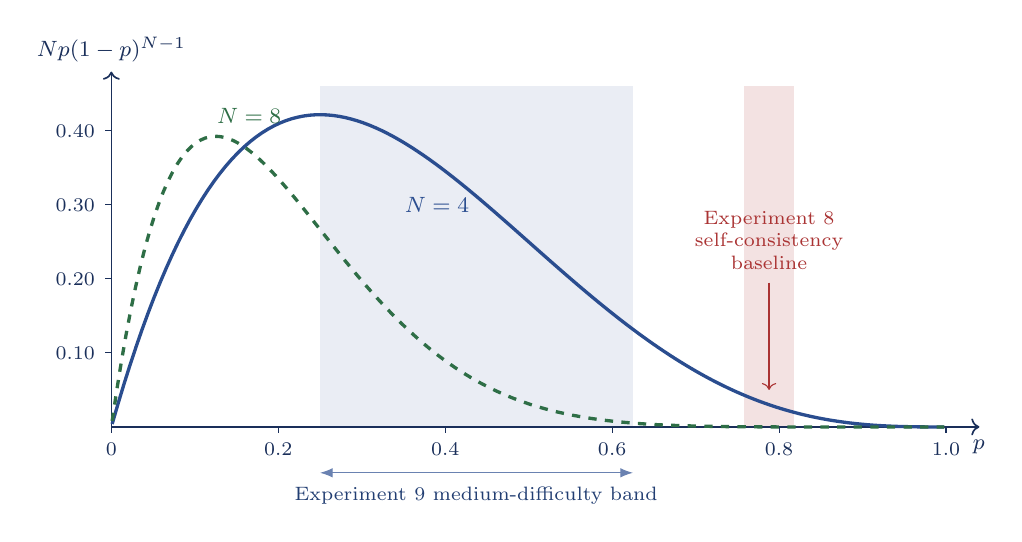
\begin{tikzpicture}[x=10.6cm,y=9.4cm,font=\footnotesize]
  % bands
  \fill[accent!10] (0.25,0) rectangle (0.625,0.46);
  \fill[failred!14] (0.758,0) rectangle (0.818,0.46);
  % axes
  \draw[->,semithick,navy] (0,0) -- (1.04,0) node[below right=1pt and -6pt]{$p$};
  \draw[->,semithick,navy] (0,0) -- (0,0.48)
    node[above,align=center,text=navy]{$N p (1-p)^{N-1}$};
  \foreach \t in {0,0.2,0.4,0.6,0.8,1.0}
    \draw[navy] (\t,0) -- (\t,-0.008) node[below,font=\scriptsize]{\t};
  \foreach \t/\l in {0.1/0.10,0.2/0.20,0.3/0.30,0.4/0.40}
    \draw[navy] (0,\t) -- (-0.008,\t) node[left,font=\scriptsize]{\l};
  % curves
  \draw[very thick,accent,domain=0.001:0.999,samples=140,variable=\x]
    plot (\x,{4*\x*pow(1-\x,3)});
  \draw[very thick,okgreen,dashed,domain=0.001:0.999,samples=180,variable=\x]
    plot (\x,{8*\x*pow(1-\x,7)});
  % labels
  \node[accent,anchor=west] at (0.34,0.30) {$N=4$};
  \node[okgreen,anchor=west] at (0.115,0.42) {$N=8$};
  \node[failred,anchor=south,align=center,font=\scriptsize]
    at (0.788,0.20) {Experiment 8\\self-consistency\\baseline};
  \draw[failred,->] (0.788,0.195) -- (0.788,0.05);
  \draw[accent!70,{Latex[length=1.6mm]}-{Latex[length=1.6mm]}]
    (0.25,-0.062) -- (0.625,-0.062);
  \node[accent!80!black,anchor=north,align=center,font=\scriptsize]
    at (0.437,-0.068) {Experiment 9 medium-difficulty band};
\end{tikzpicture}
\caption{Where a selector can beat plurality voting. The curves plot
$N p (1-p)^{N-1}$, the probability that exactly one of $N$ independent
candidates is correct, which is the canonical row a perfect selector wins and
majority voting loses. Experiment 8 placed its headline comparison against a
self-consistency baseline running at $p \in [0.758, 0.818]$ (red band), where
the quantity is 0.043 to 0.020 at $N=4$, one or two rows of a 33-row audit.
Experiment 9 moves the headline onto the model-estimated medium-difficulty band
$p \in [0.25, 0.625]$ (blue band), where at $N=8$ it runs from 0.267 at
$p=0.25$ to 0.005 at $p=0.625$. The room is real but concentrated at the
lower end of the band, which is why Experiment 9 also reports every difficulty bin
and a pooled test rather than the headline alone.}
\label{fig:headroom}
\end{figure}

\begin{figure}[htbp]
\centering
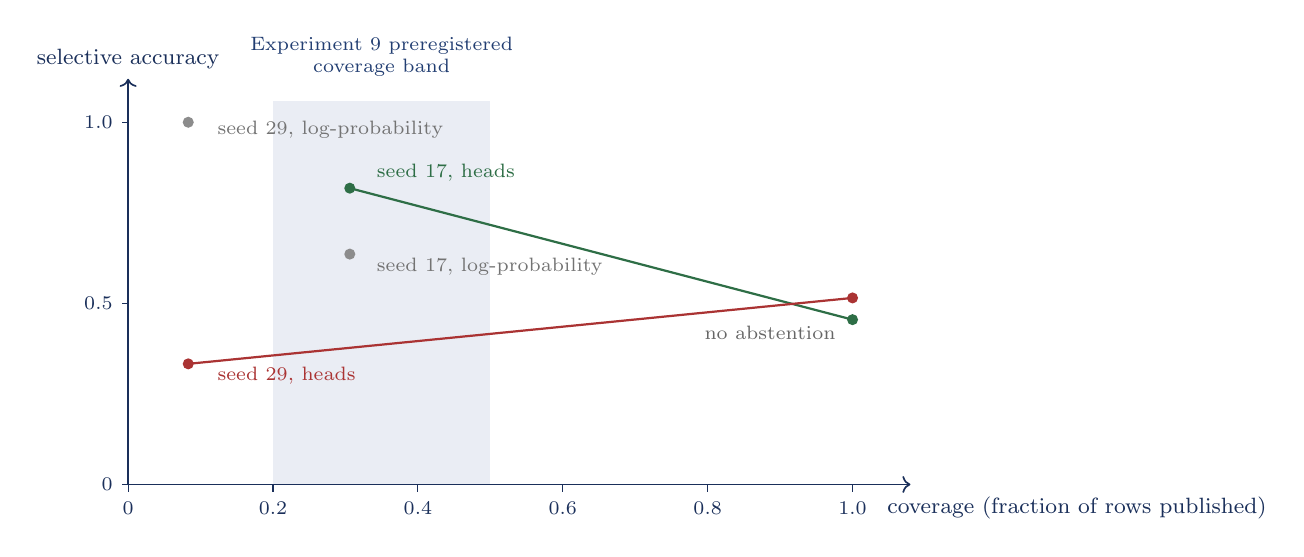
\begin{tikzpicture}[x=9.2cm,y=4.6cm,font=\footnotesize]
  \fill[accent!10] (0.20,0) rectangle (0.50,1.06);
  \draw[->,semithick,navy] (0,0) -- (1.08,0)
    node[below right=1pt and -12pt]{coverage (fraction of rows published)};
  \draw[->,semithick,navy] (0,0) -- (0,1.12)
    node[above,align=center,text=navy]{selective accuracy};
  \foreach \t in {0,0.2,0.4,0.6,0.8,1.0}
    \draw[navy] (\t,0) -- (\t,-0.022) node[below,font=\scriptsize]{\t};
  \foreach \t in {0,0.5,1.0}
    \draw[navy] (0,\t) -- (-0.008,\t) node[left,font=\scriptsize]{\t};
  % seed 17
  \draw[okgreen,thick] (0.306,0.818) -- (1.0,0.455);
  \fill[okgreen] (0.306,0.818) circle (2pt);
  \fill[okgreen] (1.0,0.455) circle (2pt);
  \fill[black!45] (0.306,0.636) circle (2pt);
  % seed 29
  \draw[failred,thick] (0.083,0.333) -- (1.0,0.515);
  \fill[failred] (0.083,0.333) circle (2pt);
  \fill[failred] (1.0,0.515) circle (2pt);
  \fill[black!45] (0.083,1.0) circle (2pt);
  \node[okgreen,anchor=west,font=\scriptsize] at (0.33,0.86) {seed 17, heads};
  \node[black!55,anchor=west,font=\scriptsize] at (0.33,0.60) {seed 17, log-probability};
  \node[failred,anchor=west,font=\scriptsize] at (0.11,0.30) {seed 29, heads};
  \node[black!55,anchor=west,font=\scriptsize] at (0.11,0.98) {seed 29, log-probability};
  \node[anchor=east,font=\scriptsize,text=black!60] at (0.99,0.42) {no abstention};
  \node[accent!80!black,anchor=south,font=\scriptsize,align=center]
    at (0.35,1.10) {Experiment 9 preregistered\\coverage band};
\end{tikzpicture}
\caption{Experiment 8 selective prediction, both seeds. Each colored line joins a
seed's published operating point to its own no-abstention accuracy; the gray
points are the log-probability baseline evaluated at the same coverage.
Seed 17 abstained at coverage 0.306 and gained 18 points over the baseline,
the program's first selective-prediction win. Seed 29's rule landed at
coverage 0.083, three published rows, where its accuracy of 0.333 loses to a
baseline that happens to be perfect on those three rows; that seed's
safe-abstention accuracy of 0.000 is over-conservatism, not miscalibration.
The claim is therefore supported on one seed of two and is not replicated.
Experiment 9 replaces that threshold rule with a split-conformal order statistic
whose realized coverage is targeted into the shaded band by construction,
which removes the failure mode seed 29 exhibits here.}
\label{fig:riskcoverage}
\end{figure}

\paragraph{Decisions taken.}
Rung 2 of the preregistered fallback ladder is invoked. The verified fan-in
claim is dead at this scale: the mechanism joins routing as proposal plus
negative evidence, and the paper's claim re-scopes to calibrated abstention
alone, with the seed split disclosed as observed rather than averaged away.
Rungs 3 and 4 explicitly did not fire, because the read-out ablation was
non-null on both seeds and the scalar publish rule stayed non-degenerate on
both; those two structural fixes are confirmed working and carry forward. The
matched plain-LoRA control and the external benchmarks were gated behind a
full gate pass and therefore remain unauthorized. Experiment 8's other
contribution is procedural: seed 17's commitment calibration and seed 29's
policy-head training reproduced the earlier crashed session
\emph{byte-identically}, with all six policy thresholds matching to full float
precision, which is the strongest determinism evidence the program has.

\paragraph{Root cause, found after the fact.}
The channel corruption has a one-line explanation, identified during the
Experiment 9 build and stated here because it is the reason Experiment 9 exists.
\texttt{Qwen3-0.6B-Base} defines no beginning-of-sequence token, so its
tokenizer's \texttt{bos\_token\_id} resolves to the end-of-text token. Experiment
8 seeded every workspace-channel teacher-forcing target and every workspace
decode with that identifier, which placed a document boundary in the middle
of the sequence. The model did the reasonable thing and began a fresh
document, which in this pretraining corpus means a fresh dialogue turn. The
causal channel never used that seed and was never affected, which is exactly
the observed damage pattern. This is a line-level defect with an
architecture-level consequence, and it was invisible to every training-time
metric because it lives only in the emission path.

\subsection{Experiment 9: Repaired channel, decoupled claims}
\label{sec:study9}

Experiment 9 was built, unit-tested and preregistered before its run, and this
section keeps that order: the design is stated first, exactly as frozen, and
the results that follow are judged against it. It responds to the two things
Experiment 8 established: a line-level defect that broke the workspace generation
channel, and a headline comparison that entangled generation quality with
selection quality and then asked both to be demonstrated on a few dozen rows.

\paragraph{Decoupling the claims.}
Experiment 8 could only ever select among workspace-channel candidates, so a
broken channel doomed the selection claim mechanically. Experiment 9 separates
three claims onto three surfaces, each independently powered.

\begin{itemize}[leftmargin=1.4em]
\item \textbf{Claim G, generation.} The repaired workspace channel reaches
  \emph{parity} with the causal channel on identical rows: zero turn-scaffold
  emissions, graded accuracy within 0.05 of causal greedy decoding, token F1
  at least 0.9 of causal, a causally live read-out (ablation drop at least
  0.05) and an open prefix gate. Parity and liveness only. At this scale
  there is no ``beats'' claim.
\item \textbf{Claim S, selection.} Verifier-weighted self-consistency beats
  plurality self-consistency on the \emph{causal-channel} pool, the same
  healthy pool the baseline votes over, so channel quality cannot contaminate
  the comparison. The heads score arbitrary token sequences by teacher-forcing
  them under the workspace prefix.
\item \textbf{Claim A, abstention.} Conformally calibrated heads beat
  mean-log-probability abstention on the risk--coverage curve over the same
  causal pool.
\end{itemize}

\paragraph{Channel repair.}
The answer channel never begins with \texttt{bos\_token\_id}; teacher-forcing
predicts the first answer token from the last hard cue token, and decoding
starts from that cue. Both channels share one prompt builder: the context
loses its trailing response header at encode time and the model appends the
header itself as hard cue tokens. The causal channel is then
$[\text{context}][\text{cue}] \rightarrow \text{answer}$ and the workspace
channel is $[\text{context}][\text{prefix}][\text{cue}] \rightarrow
\text{answer}$, so the two differ only by the latent prefix
(Figure~\ref{fig:channel}). Position zero remains a hard token, the prompt
always ends in hard tokens, and the prefix sits adjacent to the cue where its
influence is largest. Context, cue and answer positions all carry the causal
mode embedding; only prefix positions carry the synthesis and private ones,
which makes the causal channel literally the workspace channel with the
prefix removed, and therefore makes the read-out ablation exact rather than
approximate. The whole prefix is scaled by a single learned gate
$\tanh(\alpha)$ with $\alpha$ initialized at $0.05$ and logged at every
evaluation boundary; the memory and summary projections move from zero
initialization to small random initialization, so the zero now lives in the
gate and the diversity and orthogonality gradients are live from the first
step instead of provably inert. On anchor steps an auxiliary term
$\beta \cdot \mathrm{KL}$ between the workspace-conditioned answer logits and
the detached causal answer logits anchors fluency, with $\beta = 0.05$ and
the read-out-liveness gate as its declared canary: too strong a $\beta$ nulls
the mechanism, and the gate is what would catch that. Decode-time banning of
scaffold tokens is deliberately \emph{not} added, so the leak gate remains a
pure measurement and a failed repair cannot hide behind a filter.

\begin{figure}[htbp]
\centering
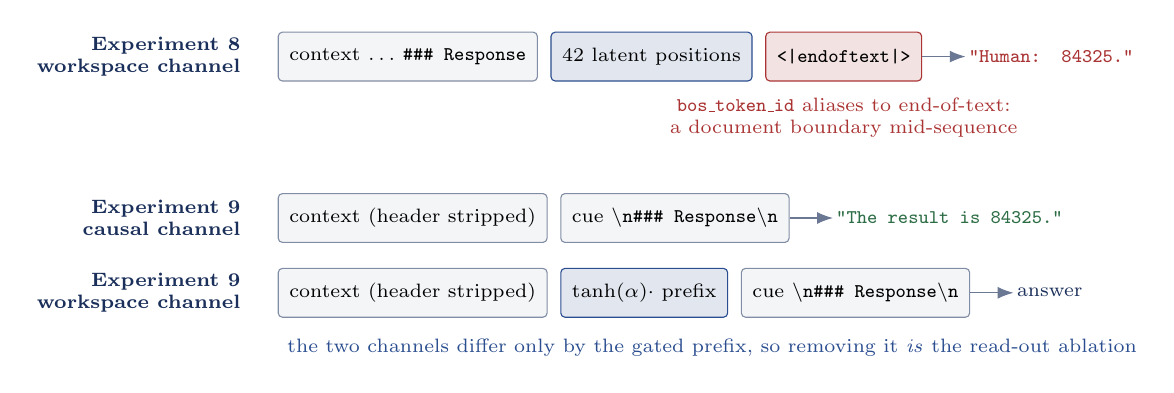
\begin{tikzpicture}[
  font=\scriptsize,
  tok/.style={draw=navy!55,fill=navy!5,rounded corners=1.5pt,
              minimum height=6.2mm,inner xsep=4pt,align=center},
  lat/.style={draw=accent,fill=accent!14,rounded corners=1.5pt,
              minimum height=6.2mm,inner xsep=4pt,align=center},
  bad/.style={draw=failred,fill=failred!14,rounded corners=1.5pt,
              minimum height=6.2mm,inner xsep=4pt,align=center},
  emit/.style={align=left,inner sep=1pt},
  lbl/.style={anchor=east,align=right,text=navy,font=\scriptsize\bfseries},
  arr/.style={-{Latex[length=2mm]},draw=navy!65}
]
% ---- row 1: Experiment 8, defective
\node[lbl] (l1) at (0,0) {Experiment 8\\workspace channel};
\node[tok,anchor=west] (a1) at (0.35,0) {context $\ldots$ \texttt{\#\#\# Response}};
\node[lat,right=1.6mm of a1] (b1) {42 latent positions};
\node[bad,right=1.6mm of b1] (c1) {\texttt{<|endoftext|>}};
\draw[arr] (c1.east) -- ++(0.55,0) node[emit,anchor=west,text=failred]
  {\texttt{"Human: 84325."}};
\node[failred,anchor=north,align=center,font=\scriptsize] at ($(c1.south)+(0,-0.9mm)$)
  {\texttt{bos\_token\_id} aliases to end-of-text:\\a document boundary mid-sequence};

% ---- row 2: Experiment 9 causal
\node[lbl] (l2) at (0,-2.05) {Experiment 9\\causal channel};
\node[tok,anchor=west] (a2) at (0.35,-2.05) {context (header stripped)};
\node[tok,right=1.6mm of a2] (c2) {cue \texttt{\textbackslash n\#\#\# Response\textbackslash n}};
\draw[arr] (c2.east) -- ++(0.55,0) node[emit,anchor=west,text=okgreen]
  {\texttt{"The result is 84325."}};

% ---- row 3: Experiment 9 workspace
\node[lbl] (l3) at (0,-3.0) {Experiment 9\\workspace channel};
\node[tok,anchor=west] (a3) at (0.35,-3.0) {context (header stripped)};
\node[lat,right=1.6mm of a3] (b3) {$\tanh(\alpha)\cdot$ prefix};
\node[tok,right=1.6mm of b3] (c3) {cue \texttt{\textbackslash n\#\#\# Response\textbackslash n}};
\draw[arr] (c3.east) -- ++(0.55,0) node[emit,anchor=west,text=navy]
  {answer};
\node[accent,anchor=north west,align=left,font=\scriptsize]
  at ($(a3.south west)+(0,-1.4mm)$)
  {the two channels differ only by the gated prefix, so removing it
   \emph{is} the read-out ablation};
\end{tikzpicture}
\caption{The Experiment 8 defect and the Experiment 9 repair. Experiment 8 seeded every
workspace teacher-forcing target and decode with \texttt{bos\_token\_id},
which \texttt{Qwen3-0.6B-Base} does not define and whose tokenizer therefore
resolves to the end-of-text token, injecting a document boundary in
mid-sequence; the model began a fresh document, which in this corpus means a
fresh dialogue turn. The causal channel never used that seed and was never
damaged, matching the observed pattern exactly. Experiment 9 removes the seed,
moves the response header out of the prompt string and into hard cue tokens
the model appends itself, and places the latent prefix between context and
cue so that the two channels form a matched pair.}
\label{fig:channel}
\end{figure}

\paragraph{Candidate machinery and conformal calibration.}
The candidate pool is $N=8$ drawn from the causal channel: one greedy
decode plus seven samples at a single temperature of $0.8$. Experiment 8's
temperature ladder is dropped because it confounds selection quality with
decode quality and, on seed 17, contributed no additional valid candidates.
The heads score every candidate by teacher-forcing it under the gated prefix,
and the publish score is
$\sigma(w \cdot [\,\text{commit},\ \text{risk},\ \text{verifier},\
\exp(\overline{\log p})\,] + b)$. The fourth feature matters: it nests the
log-probability baseline inside the combiner, so a win is a win over
something the combiner could have simply copied. Weighted self-consistency
clusters candidates by answer signature and weights each cluster by the sum
of its members' publish scores; plain self-consistency is the same rule with
unit weights, and tie rates are reported. Policy-head training and
calibration both harvest from this same pool configuration, which makes the
heads on-policy with respect to the audit.

Calibration uses 256 validation anchors split by episode-id hash into halves
$A$ and $B$ of 128. The combiner $(w,b)$ is fitted on split $A$; on split $B$
each anchor contributes one score, and the threshold is the $k$-th smallest
with $k = \lfloor (n_B+1)(1-c) \rfloor$ at $c = 0.35$, inflated so that
realized coverage is at least 0.25 with about 95\% probability. If more than
20\% of split-$B$ scores tie at the $k$-th order statistic, a preregistered
randomized tie-break applies. There is no midpoint fallback: that is the road
that produced seed 29's coverage of 0.083, and if the combiner cannot fit,
the run reports calibration failure.

\paragraph{Lanes, infrastructure and budget.}
The lanes get one structural last chance. Lane 0's brief now pools the first
half of the context positions and lane 1's the second half, which makes the
inputs asymmetric by construction rather than by penalty; the lane
projections are randomly initialized at distinct scales, so the existing
squared-cosine orthogonality pressure has a gradient for the first time. The
preregistered exit is unconditional: a mean lane-summary cosine of 0.90 or
above would be the eighth such failure, and the lanes are then demoted to a
single lane and this paper's lane-diversity sections join routing and fan-in
as proposal plus negative evidence. No further lane fixes are authorized.
A key--value cache in the decode paths, with cached post-RoPE keys and
threaded absolute positions, is what affords an audit of 320 rows instead of
64: all 256 test behavior anchors plus 64 text-to-SQL rows. Difficulty bins
are computed from the same eight samples used by every arm (easy is pass@1
above 5/8, medium is $[2/8, 5/8]$, hard is below 2/8), which is
label-dependent stratification and is disclosed as such; the headline runs on
the medium bin and every bin plus the pooled result is reported. The training
canary now exercises the workspace decode path and counts scaffold leaks,
which Experiment 8's canary could not see. The trainable-parameter delta against
Experiment 8 is one scalar and a set of re-initializations, under 0.1\%.

\paragraph{Gates, pre-mortem and the binding ladder.}
The battery is 24 gates: six on training and heads, six on Claim G, five on
Claim S, five on Claim A and two general. The Claim S headline,
verifier-weighted self-consistency beating plurality self-consistency on the
medium bin, additionally requires a pooled one-sided McNemar mid-$p$ below
0.05 on the discordant pairs for the replication verdict, is recomputed
anchors-only as a sensitivity check against the text-to-SQL rows distorting
the bin, and is guarded by a \emph{heads\_not\_logprob} check requiring the
Spearman correlation between publish score and mean log-probability to stay
below 0.95 in absolute value. A \emph{selection\_headroom\_present} gate
requires at least 10\% of medium-bin rows to have exactly one correct
candidate among the eight; if that gate fails, Claim S is declared void for
lack of headroom, which is a design result about the difficulty of the rows
rather than a failure of the model. Claim A requires audit coverage inside
$[0.20, 0.50]$, an AUGRC advantage over the log-probability baseline in at
least 90\% of 1{,}000 paired bootstrap resamples per seed, a Clopper--Pearson
95\% upper bound on selective risk no worse than 0.45, and the safe-abstention
probes. Fifteen predicted failure modes are recorded in advance, each with a
detector and a response fixed before the run; among them, an attenuated
prefix, a KL anchor strong enough to null the mechanism, a gate that never
opens, a threshold landing in a tie mass, a coverage band missed on one seed,
numerical drift from the new cache, and a weighted-self-consistency win that
turns out to be length bias rather than verification.

The ladder is binding and has five rungs. A full pass on the cores of G, S
and A authorizes the matched plain-LoRA control immediately, and nothing else
authorizes it. If G passes and S fails with headroom present, selection joins
the negative evidence and Claim A stands or falls on its own gates. If G
passes and S is void for lack of headroom, the selection question moves to
harder rows in the benchmark kit rather than being rerun at this difficulty.
If G fails on parity or leak, the latent-workspace generation channel is
falsified at this scale even with a repaired interface, the program's
generative claim ends, and head and abstention work continues on the causal
channel alone. If A fails on both seeds while G passes, the abstention claim
dies and Experiment 9 is reported as the terminal negative result for calibrated
selective prediction at 0.6B. There is no rung on which the program is
allowed to declare success by narrative.

\paragraph{Outcome.}
Experiment 9 ran as a single dual-seed session, 4{,}224 of 4{,}224 microsteps per
seed with zero skipped optimizer updates, followed by fresh-process audits of
320 rows per seed at roughly 19 seconds per row. Both seeds failed the
battery at 17 of 24 gates, with six of the seven failures shared, and the
shared six state one result twice: every repair in the experiment worked and
replicated, and every mechanism the repairs were built to expose measured
null or lost to its training-free baseline, and that replicated too.
Table~\ref{tab:study9} carries the headline rows. One session defect is
disclosed up front: after both audits and both gate computations had completed
and been written to disk, the notebook crashed in a display-only cell that
referenced a Experiment 8 record field name, so the pooled selection statistic and
the archive bundles were recomputed offline from the on-disk artifacts using
the preregistered formulas, and the mid-training metrics logs were fetched
from the run's storage and byte-verified against the training heartbeat
before use.

\begin{table}[htbp]
\caption{Experiment 9 held-out results. Audits are 320 rows per seed: all 256 test
behavior anchors plus 64 text-to-SQL rows, decoded fresh from checksummed
checkpoints. Red marks preregistered gate failures.}
\label{tab:study9}
\centering\footnotesize
\begin{tabularx}{\textwidth}{@{}Xccc@{}}
\toprule
\textbf{Measurement} & \textbf{Seed 17} & \textbf{Seed 29} & \textbf{Interpretation} \\
\midrule
Completed microsteps / skipped updates & 4{,}224 / 0 & 4{,}224 / 0 & Training was stable on both seeds. \\
Turn-scaffold leak, 320 audited rows & 0 & 0 & The register repair held on the emission path. \\
Causal minus workspace greedy accuracy & $+0.013$ & $-0.003$ & Experiment 8's thirty-point channel gap is gone. \\
Workspace / causal token F1 ratio & 1.015 & 1.025 & The workspace channel writes marginally cleaner text. \\
Memory-token ablation (34 of 42 positions) & \fail{0.000} & \fail{$-0.022$} & Removing the latent memory costs nothing. \\
Prefix gate $\tanh(\alpha)$, full-run range & 0.0500--0.0507 & 0.0498--0.0504 & Flat by construction; disqualified as evidence (see text). \\
Medium-bin exactly-one-correct fraction & \fail{0.000} & \fail{0.000} & Claim S void for headroom, as preregistered. \\
Weighted vs.\ plurality SC discordant pairs & 0 / 0 & 2 / 0 & Two flipped votes in 640 rows; pooled mid-$p$ 0.125. \\
Conformal coverage, band $[0.20, 0.50]$ & 0.244 & \fail{0.188} & The floor held on one seed, missed by 0.013 on the other. \\
Published answers correct & 78 / 78 & 60 / 60 & Perfect selective precision at both operating points. \\
AUGRC, heads vs.\ log-probability & \fail{0.0637 / 0.0594} & \fail{0.0654 / 0.0623} & The free baseline wins on both seeds. \\
Mean lane-summary cosine & \fail{0.940} & \fail{0.975} & Lane failures eight and nine; demotion executes. \\
Gates passed & 17 / 24 & 17 / 24 & Both seeds fail; the ladder decides, not the narrative. \\
\bottomrule
\end{tabularx}
\end{table}

\paragraph{The repairs held.}
The scaffold leak that defined Experiment 8 is gone: zero leaked rows in 640
audited decodes, and the training canary, which now exercises the workspace
decode path, recorded a zero format-marker rate at seventeen of eighteen
evaluation boundaries across both seeds, with one transient one-in-eight
reading on seed 29 during the local phase, absent thereafter. Channel parity
followed: workspace-conditioned greedy decoding matched causal decoding to
within 0.013 on seed 17 and exceeded it by 0.003 on seed 29, with token-F1
ratios above one on both. The bos/end-of-text diagnosis of
Section~\ref{sec:study8} is thereby confirmed at 320-row scale on two seeds:
remove the seeded identifier and the channel damage vanishes entirely. The
conformal machinery also did what it was introduced to do. Both seeds fitted
non-degenerate four-feature combiners with thresholds taken from the held-out
half, tie mass 0.008 and no jitter needed, and realized audit coverage landed
at 0.244 and 0.188 against Experiment 8 publish coverages of 0.172 and 0.078.
Seed 29's 0.188 sits 0.013 below the preregistered band and fails its gate;
the pre-mortem named a one-seed band miss in advance, and the shortfall is
validation-to-test shift, not a return of the degenerate-threshold pathology.

\paragraph{The read-out is inert, and the instruments needed correcting first.}
Two instrument corrections from a post-session code audit are disclosed ahead
of the finding, because both had initially overstated it. First, the shipped
ablation did not remove the whole prefix: it sliced away the 34 memory
positions and kept the 8 gated synthesis tokens in both arms, so the measured
0.000 and $-0.022$ changes in graded accuracy, with token-F1 changes of
0.0003 and $-0.003$, bound the memory tokens only. The full prefix is bounded
by the stronger instrument, channel parity: the causal arm \emph{is} the
workspace arm with the entire prefix removed, and it sits within 0.013 of it
on both seeds. Second, the flat gate trajectory
(Figure~\ref{fig:gatetrace}) is not evidence that training rejected the
prefix, because the gate could not have moved either way: the first operation
the frozen model applies to the gated embeddings is a root-mean-square
normalization, which is scale-invariant, so the attention-visible content of
the prefix is independent of $\alpha$ for any positive value, and the loss
gradient on the gate through that dominant branch is approximately zero
whether or not the prefix is useful. The channel was open at its
initialization, and the decoder ignored its content through attention. A
third design fact completes the diagnosis: the fluency anchor's reference
distribution is this same model on the same inputs with the prefix removed,
so at convergence of the answer loss the only persistent gradient on the
prefix pathway points exactly at changing the logits by nothing. With both
channels conditioned on the same full context, the latent was redundant by
construction. Experiment 8's non-null ablation is reinterpreted as the removal of
a \emph{corrupting} prefix rather than an informative one, and the
mechanism-level conclusion survives the corrections in sharpened form: the
model can minimize its loss while ignoring the workspace, and it does.
Parity, the one Claim G surface that passed, was achieved by irrelevance.

\begin{figure}[htbp]
\centering
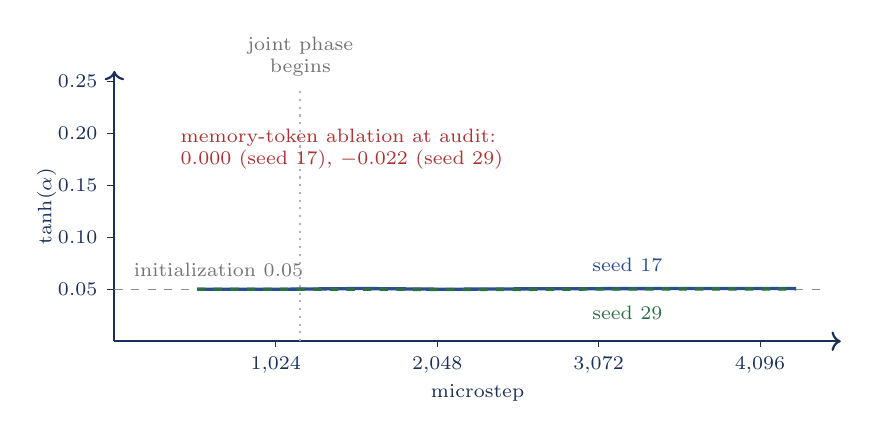
\begin{tikzpicture}[x=2.05cm,y=13.2cm,font=\footnotesize]
  % axes
  \draw[->,thick,navy] (0,0) -- (4.5,0);
  \draw[->,thick,navy] (0,0) -- (0,0.26);
  \node[navy,font=\scriptsize,anchor=north] at (2.25,-0.032) {microstep};
  \foreach \t/\l in {1/1{,}024, 2/2{,}048, 3/3{,}072, 4/4{,}096}
    \draw[navy] (\t,0) -- (\t,-0.006) node[below,font=\scriptsize]{\l};
  \foreach \t/\l in {0.05/0.05, 0.10/0.10, 0.15/0.15, 0.20/0.20, 0.25/0.25}
    \draw[navy] (0,\t) -- (-0.045,\t) node[left,font=\scriptsize]{\l};
  \node[rotate=90,navy,font=\scriptsize] at (-0.42,0.13) {$\tanh(\alpha)$};
  % init line
  \draw[black!45,dashed] (0,0.05) -- (4.4,0.05);
  \node[font=\scriptsize,text=black!55,anchor=south west] at (0.06,0.053)
    {initialization $0.05$};
  % joint phase divider
  \draw[black!30,dotted,thick] (1.152,0) -- (1.152,0.245)
    node[above,font=\scriptsize,text=black!55,align=center]{joint phase\\begins};
  % seed 17
  \draw[very thick,accent] plot coordinates
    {(0.512,0.0500)(1.024,0.0500)(1.536,0.0507)(2.048,0.0500)(2.560,0.0504)
     (3.072,0.0506)(3.584,0.0507)(4.096,0.0507)(4.224,0.0507)};
  % seed 29
  \draw[very thick,okgreen,dashed] plot coordinates
    {(0.512,0.0500)(1.024,0.0500)(1.536,0.0501)(2.048,0.0498)(2.560,0.0499)
     (3.072,0.0503)(3.584,0.0504)(4.096,0.0504)(4.224,0.0504)};
  \node[accent,anchor=south west,font=\scriptsize] at (2.9,0.058) {seed 17};
  \node[okgreen,anchor=north west,font=\scriptsize] at (2.9,0.043) {seed 29};
  % annotation
  \node[failred,anchor=west,align=left,font=\scriptsize] at (0.35,0.185)
    {memory-token ablation at audit:\\$0.000$ (seed 17), $-0.022$ (seed 29)};
\end{tikzpicture}
\caption{The prefix gate is structurally silent. $\tanh(\alpha)$ at every
evaluation boundary of the Experiment 9 run, plotted on the range $[0, 0.26]$; a
fully open gate would sit near 1.0, far off scale. The trajectory moves less
than 0.0008 on both seeds, but this flatness is forced rather than
informative: the frozen model normalizes the gated embeddings before
attention, so the content visible to the decoder is independent of $\alpha$
and the gradient on the gate is approximately zero whether or not the prefix
helps. The gate is retained as telemetry and disqualified as evidence; the
read-out finding rests on channel parity and the memory-token ablation,
annotated in red.}
\label{fig:gatetrace}
\end{figure}

\paragraph{Selection was void, as its own gate anticipated.}
The realized audit difficulty is bimodal, not banded: 187 and 189 of 320 rows
are easy, with all eight candidates correct and every arm at 1.000; 91 and 98
rows are hard, with any-valid oracles of 0.143 and 0.122; and the medium
strata of 42 and 33 rows contain no exactly-one-correct rows at all, so
\emph{selection\_headroom\_present} fails at 0.000 on both seeds and Claim S
is void for lack of headroom, the design outcome the gate was written to
name. The weighting itself was nearly inert: verifier-weighted and plurality
self-consistency produced zero discordant pairs on seed 17 and two on seed
29, two flipped votes in 640 rows, for a pooled McNemar mid-$p$ of 0.125.
Report-only signals are recorded without weight: on medium rows the
head-argmax arm beat greedy on both seeds, 0.786 against 0.643 and 0.818
against 0.697, with best-of-$N$ log-probability comparable, which is
consistent with selection signal existing at difficulty strata this audit
barely samples. Per the void rung, the selection question moves to rows with
measured headroom rather than being rerun at this difficulty.

\paragraph{Abstention failed its comparison and honored its contract.}
The preregistered Claim A comparison is lost on both seeds: heads AUGRC
0.0637 and 0.0654 against log-probability 0.0594 and 0.0623, with
paired-bootstrap win fractions of 0.13 and 0.179 against the 0.90
requirement. The guard gates passed, which makes the loss informative rather
than degenerate: Spearman correlation between publish score and mean
log-probability is 0.830 and 0.821, under the 0.95 ceiling, so the heads are
not a re-derivation of likelihood; they are simply not better than it on this
distribution. The operating points themselves replicated exactly for the
first time in the program: 78 of 78 and 60 of 60 published answers correct,
selective-risk upper bounds of 0.038 and 0.049, safe-abstention probes at
1.000, and commit coverage of exactly 0.000 on text-to-SQL on both seeds, the
one audited domain where the model is incompetent, with quality 0.078 and
0.109, which is also what drags the pooled quality gate to 0.663 and 0.666
against its 0.70 floor. The shape of the loss is instructive: with 58 to 59
percent of audit rows trivially easy, the log-probability curve is near
ceiling on much of its length, and a coarse, near-binary score can win its
operating point while losing an area metric. We report the operational
property and decline to rename it a victory.

\paragraph{The remaining failures.}
The verifier head ranked corrupt above clean at 0.944 and 0.947 on
teacher-forced features and inverted to $-0.233$ and $-0.297$ on freshly
generated audit emissions, the program's cleanest instance yet of
train-to-generation distribution shift in a learned judge. The on-policy
validity floor was unmet on both seeds: 1{,}024 emission attempts yielded 2,
5 and 2 valid positives on one seed and 1, 2 and 5 on the other for the
numeric, ordering and unit families, against a floor of 16 each, so the heads
trained on roughly 25 positives against 1{,}000 negatives. A post-session
code audit reclassified this failure as an implementation defect at least as
much as model incapacity: the harvest generated from the training collator's
fixed-length padded prompt surface, roughly 150 padding tokens inserted
between prompt and response cue, while the audit encodes prompts unpadded,
and on the audit surface the same anchor families reach causal validity of
0.82. The same padded surface feeds calibration, which plausibly contributes
to seed 29's validation-to-test coverage shift. A
preregistration-versus-implementation gap is also disclosed here rather than
left to a reader: the plan text describes the corresponding gate as enforcing
the validity floor, while the shipped gate only requires that head training
occurred, so the gate records a pass over a floor that was not met. Lane-summary cosines
of 0.940 and 0.975 are lane-diversity failures eight and nine; the
unconditional exit executes, the design drops to a single lane, and this
paper's lane sections join routing and fan-in as proposal plus negative
evidence.

\paragraph{Decisions taken.}
The executable preregistration, the notebook inside the sha-verified bundle,
enumerates a dead read-out in its stop rung; the prose ladder above, frozen
later, words that rung as parity or leak. The older executable document
governs, the wording gap is disclosed here, and the stop rung applies. The
generative read-out mechanism is retired at this scale, which makes the
score zero for three: all mechanisms proposed in Section~\ref{sec:design}
have now taken preregistered tests and failed them. The matched plain-LoRA
control remains unauthorized, nine experiments and zero full passes, and the
external benchmarks remain gated behind it. What this experiment adds beyond the
retirements is a constraint that any successor inherits: the failure was not
corruption, capacity, or optimization instability, each of which was
individually repaired or ruled out along the way, but redundancy. A successor
workspace claim must make the latent structurally necessary, for instance by
an information asymmetry in which the causal channel does not see everything
the workspace sees, so that ignoring the latent costs loss, and it must
preregister that necessity check as its first gate.

\subsection{Experiment 10: The necessary channel}
\label{sec:study10}

Experiment 9 ended with a constraint: a successor workspace claim must make the
latent structurally necessary, so that ignoring it costs loss, and must
preregister that necessity check as its first gate. Experiment 10 is that
successor, built and preregistered before its run. On \emph{masked} behavior
anchors, the operative premise is moved out of the request the answer path
reads: the decoder's input ids for the answer channel physically lack the
operands, the workspace encoder alone sees the full context, and the only
route from the premise to the answer is the latent. Training itself uses the
same asymmetry on alternating batches, so a model that ignores the latent
pays cross-entropy for it during training, not only at audit. The design
carries the accumulated instrument corrections forward: the read-out is
re-pointed at the evidence encoding rather than the private canvas, the
scale-invariant prefix gate is deleted and its telemetry retained without
evidentiary weight, the fluency anchor is flipped from the prefix-free
reference (measured in Experiment 9 as directed pressure to close the channel) to
a distillation teacher, the harvest and calibration surfaces are unpadded
(closing Experiment 9's disclosed padded-surface defect), the validity floor is a
real gate rather than a recorded aspiration, LoRA extends to all layers
(132.2M trainable against Experiment 9's 76.6M, disclosed), and anchor difficulty
is parameterized (chain length, operand digits, distractors) with the audit
pool banded by pass@32 under a frozen estimator whose 224 row ids are fixed
before training. Auxiliary instruments are added on both sides of the
question: a latent-only linear probe trained to decode the withheld premise,
a \emph{trained} gist attribution control (a matched prefix trained on
alternating batches with no evidence access), and a within-family
shuffled-prefix arm as the primary necessity control. The battery is 22
gates; the binding ladder's rung 1, a dead channel under structural
necessity, is preregistered as terminal for the generative mechanism.

\paragraph{Session record.}
The first launch crashed at rung 0: both seeds completed all 3{,}200
microsteps and on-policy collection, then died at the same line inside
calibration, where the publish-rule fitter retained Experiment 9's three-or-four
feature guard while the preregistered form selection fits four- and
five-feature rules. The two-line fix and a regression test covering the
exact call were applied, the bundle rebuilt (only the trainer, its test file
and the manifest changed; all data files CRC-identical), and the relaunch
resumed from the crashed run's step-3{,}200 checkpoints, which carry
optimizer, scaler, and python/torch/cuda RNG state. The resume is
bit-equivalent to an uninterrupted run: the on-policy collection counts
reproduced digit-for-digit (41 and 43 valid emissions of 512, with identical
per-family splits). One gate artifact follows from the salvage and is
disclosed rather than counted: the canary-cleanliness gate reads the
resumed process's metrics log, which contains only the resume marker, so it
records false on both seeds; recomputing the gate's exact rule on the
original training logs gives seven canary records per seed, zero dirty
boundaries, zero prompt leaks. The effective battery result is 15 of 22
gates per seed, with seven real failures, identical across seeds.

\begin{table}[htbp]
\caption{Experiment 10 held-out results. Audits are 288 rows per seed (224 banded
anchors, of which 99 are masked, plus 64 text-to-SQL); the audit pool was
banded by a frozen pass@32 estimator before training. Red marks preregistered
gate failures.}
\label{tab:study10}
\centering\footnotesize
\begin{tabularx}{\textwidth}{@{}Xccc@{}}
\toprule
\textbf{Measurement} & \textbf{Seed 17} & \textbf{Seed 29} & \textbf{Interpretation} \\
\midrule
Completed microsteps / skipped updates & 3{,}200 / 0 & 3{,}200 / 0 & Training stable; resume bit-exact. \\
Masked-row leak (99 rows) / causal floor & 0 / 0.000 & 0 / 0.000 & The necessity instrument is airtight. \\
Masked workspace accuracy & \fail{0.000} & \fail{0.000} & The only path carried nothing usable. \\
Trained gist-control accuracy (masked) & 0.000 & 0.000 & Not an attribution artifact. \\
Premise probe accuracy (bar 0.50) & \fail{0.297} & \fail{0.334} & The latent holds traces generation cannot spend. \\
Unmasked parity gap (workspace $-$ causal) & $+0.037$ & $0.000$ & The workspace does no harm; seed 17's is better. \\
Verifier margin on generated candidates & \fail{$-0.277$} & \fail{$-0.227$} & Train-to-generation shift persists in the judge. \\
On-policy validity floor (16/family) & \fail{41 / 512} & \fail{43 / 512} & Numeric and unit generation weak at banded difficulty. \\
Conformal coverage, band $[0.20, 0.55]$ & 0.295 & 0.267 & Experiment 8's strangle stays fixed; both seeds in band. \\
Published answers correct & 83 / 85 & 77 / 77 & Selective risk UCB$_{95}$ 0.072 and 0.038. \\
Partial AUGRC, heads vs.\ log-probability & 0.0128 / 0.0156 & 0.0073 / 0.0114 & Heads better on \emph{both} seeds, a program first. \\
Paired-bootstrap win fraction (bar 0.80) & \fail{0.746} & \fail{0.792} & Directionally consistent, short of the bar by 0.054 / 0.008. \\
Gates passed (of 22; canary artifact excluded) & 15 & 15 & Rung 1: terminal for the generative mechanism. \\
\bottomrule
\end{tabularx}
\end{table}

\paragraph{The necessity result.}
Every alternative explanation the program has previously needed was ruled
out by the run itself. The masking held: zero leaked premise literals in 198
masked audits under a line-anchored scanner shared by trainer and audit. The
floor held: with the prefix removed, masked accuracy is exactly 0.000, so
the question is only answerable through the channel. The attribution control
held: a trained gist prefix with no evidence access also reads 0.000, so
nothing generic about trained prefixes explains a success, had one occurred.
Unmasked parity held on both seeds, with seed 17's workspace arm above its
causal arm (0.508 against 0.471), so the machinery does not damage the rows
it cannot help. Against that instrument, the reading is zero: masked
workspace accuracy 0.000 on 99 rows per seed, on both seeds, while the
latent-only probe decodes 0.297 and 0.334 of the withheld premise. Experiment 9
showed the latent was ignored when redundant; Experiment 10 shows it is
\emph{still} unusable when it is the only source, even though the
information demonstrably reaches the latent state. The ladder's terminal
rung executes: the generative workspace mechanism is retired at this scale,
now under structural necessity rather than redundancy.

\paragraph{What the near-miss preserves.}
The calibrated-commitment stack recorded its strongest experiment. Conformal
coverage landed inside the band on both seeds, the fitted publish rules were
continuous (329 and 372 distinct scores), the operating points published 83
of 85 and 77 of 77 correct answers with selective-risk upper bounds of 0.072
and 0.038, and, for the first time in the program, the heads' risk--coverage
curve beat matched mean-log-probability abstention on both seeds in the
preregistered coverage band, at paired-bootstrap win fractions of 0.746 and
0.792 against the 0.80 bar. The win fraction is a one-sided $p$-value in
disguise, and at 288 audit rows per seed the design could only have detected
an effect roughly three times the observed size; the claim therefore closes
unestablished with a recorded effect direction, an effect size, and a power
analysis, and any successor inherits an audit-set requirement in the
thousands of rows, not hundreds. The verifier head repeated Experiment 9's
distribution shift, ranking teacher-forced features correctly while
inverting on freshly generated candidates ($-0.277$ and $-0.227$), and the
on-policy validity floor was genuinely unmet at banded difficulty (41 and 43
valid of 512 attempts, concentrated in the abstention and ordering
families), which is now a measured property of the generation channel rather
than a padded-surface artifact.

\paragraph{The sharpened constraint.}
Experiment 9's lesson was necessity; Experiment 10's is that necessity is not
sufficiency. The probe-positive, generation-zero signature that survived
every repair in this program is, in retrospect, the published failure mode
of answer-only supervision on latent reasoning tokens: CODI's ablation
reproduces it exactly, with GSM8k accuracy collapsing from 43.7 to 24.5 when
its hidden-state distillation term is removed while the latent remains
present and trained~\cite{codi2025}, and Coconut documents the same class at
the same scale~\cite{coconut2024}. Every published system that does pass
content through a latent interface into a frozen decoder shares one
ingredient no HLWM experiment had: a dense, token-level objective through the
latent itself, reconstruction or distillation, whose targets cannot be
predicted without the latent's content. This program's experiments supervised
the answer and hoped the latent would become useful; ten experiments say it does
not, at this scale, under either redundancy or necessity. A successor
preregistration exists that combines the retained necessity instrument with
dense latent supervision and per-latent targets; it is a new program with
its own gates and is not claimed here.

\subsection{A preregistered successor: the dense-supervision channel}
\label{sec:successor}

The necessity experiment sharpened the constraint on any successor: making
the latent the only carrier of required information makes its failure
measurable, and it fails; the missing ingredient, shared by every published
system that does pass content through a latent interface into a frozen
decoder, is a dense token-level objective through the latent
itself~\cite{codi2025,coconut2024}. A successor instantiation implementing
that constraint is built, unit-gated, and preregistered; its on-device
preflight has passed on the target hardware, and its run had not completed
at the time of writing. We describe it here because it is the architecture
of Figure~\ref{fig:architecture} in its current form, and because its
design is the direct product of the failure record above. No result from it
is claimed in this paper.

Four changes define the successor (Figure~\ref{fig:densesup}). First, the
workspace produces six autoregressive \emph{continuous thoughts}: the
model's own last hidden state, projected through a small trained map and
rescaled to the base embedding distribution, re-enters as the next input
embedding, so latents are decoder-legible by construction rather than by
hope. Second, every latent position receives direct supervision. A teacher
pass conditions on the gold reasoning trace and its per-layer hidden states
at the answer position become distillation targets for the student pass,
which sees only the masked prompt and its own thoughts; each thought must
additionally decode its assigned trace segment through the frozen unembedding,
and the thoughts jointly must reconstruct the withheld premise from a
standing start. Third, the interface moves from an input-embedding splice to
per-layer key--value slots behind post-softmax gates initialized
small-positive, so no normalization layer can silence the gradient and no
weight-decay term can close the channel unopposed, the two mechanisms behind
the earlier inert-gate results. Fourth, specialist capacity is routed
deterministically by task family, with a detached probe learning to recover
the route: load balance is a property of the data loader, and the collapse
mode that retired the learned router cannot recur because nothing about the
assignment is learned. Every mechanism ships with a blocking on-device
preflight (gradient liveness of each loss group, gate-closed equivalence,
decode--train parity, memory and throughput gates), and the audit adds
paired controls, within-family shuffled thoughts, compute-matched
content-free thoughts, slot ablation, and cross-routed experts, so that a
positive masked-transfer reading cannot be manufactured by any single
confound the program has previously encountered.

\begin{figure}[htbp]
\centering
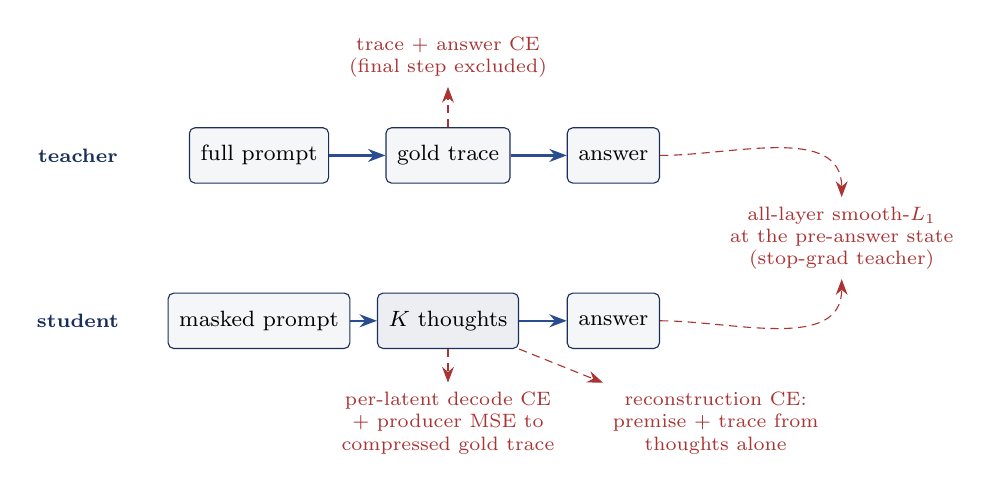
\begin{tikzpicture}[
  font=\footnotesize,
  seg/.style={draw=navy, rounded corners=2pt, align=center, inner sep=4pt, minimum height=2em},
  frozen/.style={seg, fill=codebg},
  trained/.style={seg, fill=navy!8},
  loss/.style={font=\scriptsize, text=failred, align=center},
  arr/.style={-{Stealth[length=2.2mm]}, thick, draw=accent},
  lossarr/.style={-{Stealth[length=2mm]}, densely dashed, draw=failred},
]
\node[font=\scriptsize\bfseries\color{navy}] at (-1.1, 1.05) {teacher};
\node[frozen] (tp) at (1.2, 1.05) {full prompt};
\node[frozen] (tt) at (3.6, 1.05) {gold trace};
\node[frozen] (ta) at (5.7, 1.05) {answer};
\node[font=\scriptsize\bfseries\color{navy}] at (-1.1, -1.05) {student};
\node[frozen] (sp) at (1.2, -1.05) {masked prompt};
\node[trained] (st) at (3.6, -1.05) {$K$ thoughts};
\node[frozen] (sa) at (5.7, -1.05) {answer};
\draw[arr] (tp) -- (tt); \draw[arr] (tt) -- (ta);
\draw[arr] (sp) -- (st); \draw[arr] (st) -- (sa);
\node[loss] (distill) at (8.6, 0) {all-layer smooth-$L_1$\\at the pre-answer state\\(stop-grad teacher)};
\draw[lossarr] (ta.east) to[out=0, in=90] (distill.north);
\draw[lossarr] (sa.east) to[out=0, in=-90] (distill.south);
\node[loss] (stepce) at (3.6, -2.35) {per-latent decode CE\\$+$ producer MSE to\\compressed gold trace};
\draw[lossarr] (st) -- (stepce);
\node[loss] (recon) at (7.0, -2.35) {reconstruction CE:\\premise $+$ trace from\\thoughts alone};
\draw[lossarr] (st.south east) -- (recon.north west);
\node[loss] (tce) at (3.6, 2.3) {trace $+$ answer CE\\(final step excluded)};
\draw[lossarr] (tt) -- (tce);
\end{tikzpicture}
\caption{Dense supervision in the successor channel. The teacher pass
conditions on the gold trace; the student pass sees only the masked prompt
and its own continuous thoughts. Every latent position carries direct
losses: per-latent decoding of its trace segment, regression to the
compressed gold embedding, standing-start reconstruction of the withheld
premise, and all-layer distillation of the teacher's pre-answer states.
Emergence is nowhere load-bearing.}
\label{fig:densesup}
\end{figure}

\subsection{Post-termination addendum: the certified run and the misaligned write}
\label{sec:certified}

This subsection was added after the program closed and reports events dated
2026-09-05 to 2026-09-07; nothing before it has been rewritten in light of it.
The successor run described above completed unattended after termination
(1{,}200 microsteps, 75 optimizer updates, zero skipped, both seeds). Its
warm-phase reconstruction gate passed on both seeds (exact match 0.596 and
0.603 against the 0.50 floor), the preregistered go/no-go then read masked
exact match 0.000 on both seeds, and the run aborted per protocol --- the
second independent abort of the dense-supervision channel at this budget
class. The post-abort audit battery ran to completion, and one number in it
changes what the failure is: the premise probe read \textbf{0.6212 and
0.7576} against 0.129 chance on 263 held-out masked rows per seed. For the
first time in the program's history the preregistered decodability bar
($\geq 0.50$) \emph{passed} while generation through the same channel
measured exactly zero on every masked-core row, with unmasked parity intact
(0.517/0.510) and zero leaked rows. The dissociation is no longer ``weakly
readable, unusable''; it is strongly readable and exactly unusable.

A preregistered analysis (plan and amendment frozen before their results
existed; both are in the repository with the run artifacts) then asked
\emph{where} the readable content sits relative to what the decoder listens
to. For each labelled masked-core row, the Jacobian of the ten digit-token
logits at the first gold-digit position was taken with respect to the six
thought embeddings; the top-8 right singular subspace of that $10 \times
6144$ map is the row's \emph{decoder-sensitive subspace}, and the audit's own
probe protocol was retrained separately on the component of the thoughts
inside that subspace and on its orthogonal complement. Instrument gates
replicated the recorded audit before any reading was taken: masked exact
match 0.000, and the held-out probe reproduced to three decimals on the
audit's own fp16/CUDA conditions. Two findings, consistent across two
environments (Apple M2/bf16 and Tesla T4/fp16):

\begin{itemize}
\item \textbf{The channel is not gradient-dead.} The Jacobian norm through
  the six thoughts is a median 0.29--0.36 of the norm through an equal count
  of real prompt tokens. The decoder listens to the thought positions.
\item \textbf{The content is not where the decoder listens.} At $n{=}160$
  rows with mean-projected features (the adjudicating reading under the
  frozen amendment, power checks passed), the probe recovers the withheld
  digit at \textbf{0.075 and 0.100} (chance 0.129) from the
  decoder-sensitive component, and at \textbf{0.400 and 0.725} from the
  orthogonal complement (same-row references 0.425 and 0.800).
\end{itemize}

The failure therefore localizes: not capacity, not liveness, not
readability, but \emph{write alignment}. The training objective stored the
premise in directions the decoder's output map is insensitive to, an
external probe read it there, and the preregistered decodability bar ---
which the run passed --- was measuring membership in the wrong subspace.
This is the constructive counterpart of the verbalizable-workspace
finding~\cite{workspace2026}: probe decodability and availability for the
model's own use are different properties, and only the second one was ever
the target. The budget caveat is unchanged --- 75 optimizer updates is two
to five orders of magnitude below published successes in this class --- so
the result is a mechanism for the failure at this budget, not a proof the
write cannot align under more training. Any successor inherits two concrete
obligations: supervise the write \emph{into} the decoder-sensitive subspace
rather than hoping dense targets land there, and audit channel liveness in
declared, token-visible form~\cite{da2026} rather than through learned
implicit gates whose alignment cannot be read off the token stream.

\subsection{Scale-up candidate: status and blocking audit}

A preregistered protocol exists for a Qwen3-8B-class candidate. It pins
\texttt{Qwen/Qwen3-8B} at revision
\texttt{b968826d9c46dd6066d109e\allowbreak abc6255188de91218} and does not transplant the
dense weights into a new randomly initialized backbone. The Qwen weights
remain resident in 4-bit NF4 form; rank-16 LoRA modules train every attention
and MLP projection, while a separately trainable FP32 HLWM sidecar supplies
two private lanes, one tied denoising transition, four routed bottleneck
experts, a learned latent prefix, a cheap difficulty gate, and publish, risk,
and candidate-error heads. Easy supervised rows mask the latent prefix and
train the direct causal route; harder rows train synthesis conditioned on the
private workspace. At a sampled corruption time, the same transition executes
two recurrent refinements rather than allocating a separately parameterized
block. Full reverse-time execution is reserved for generation and verifier
training.

The data boundary is stricter than the earlier Reasoning9000 release.
Existing episodes contribute only prompts, context, and constraints. Two
distinct candidate teachers answer independently; a third model critiques and
corrects them while constructing a named hard negative; two further judges
must both accept the corrected answer and confirm that the negative is wrong.
Every provider response is checkpointed immediately, disagreement fails
closed, lineage groups remain split-isolated, and the main 8B launch is
disabled until at least 25,000 accepted teacher packets exist. Deterministic
arithmetic, conversion, ordering, and missing-evidence anchors are appended
separately for execution checks and on-policy labels; they do not substitute
for broad independent adjudication. Table~\ref{tab:8b} summarizes the
protocol commitments.

\begin{table}[htbp]
\caption{Preregistered Qwen3-8B candidate protocol. These are implementation
commitments, not observed results.}
\label{tab:8b}
\centering\footnotesize
\begin{tabularx}{\textwidth}{@{}>{\raggedright\arraybackslash}p{0.17\textwidth}XX@{}}
\toprule
\textbf{Component} & \textbf{Committed setting} & \textbf{Failure boundary} \\
\midrule
Backbone adaptation & Pinned Qwen3-8B; NF4 double quantization; rank-16 LoRA on \texttt{q/k/v/o/gate/up/down} projections. & No claim of a from-scratch model or full-weight conversion. \\
Native sidecar & Latent width 384; two 16-token lanes; four experts; four diffusion times; two tied refinements; four prefix tokens. & A sidecar that does not improve a compute-matched Qwen control is removed. \\
Distributed execution & One model trained by two DDP processes on two 15\,GB T4 GPUs. & Both devices must pass the real-model forward/backward preflight. \\
Training phases & Joint causal, denoising, routing, diversity, difficulty, and paired-policy losses; then generated training-anchor policy updates. & Validation and test labels may not enter gradient updates. \\
Persistence & Atomic checksummed adapter, sidecar, optimizer, scheduler, scaler, per-rank RNG, phase, and exact microstep; time, signal, and stop-file exits. & A checksum, run-signature, data-snapshot, or world-size mismatch blocks resume. \\
Evaluation & Validation-only publish calibration; untouched test anchors; original Qwen versus adaptive HLWM quality, latency, peak allocation, tokens/s, power, and watt-hours/output. & A failed gate is reported as a failed candidate, not relabeled production-ready. \\
\bottomrule
\end{tabularx}
\end{table}

Kaggle sessions use an 8.5-hour run budget with a 20-minute save buffer,
periodic atomic checkpoints, an explicit stop file, and optional
synchronization to a private model repository. Numbered checkpoint parts
provide a second recovery path when remote synchronization is unavailable.
The frozen data manifest carries row counts and SHA-256 hashes for all three
splits; the checkpoint stores the matching aggregate fingerprint and refuses
a changed snapshot. This protocol reduces repeated manual intervention and
artifact loss, but it does not make intermittent free hardware equivalent to
a controlled training cluster.

The first narrow capability gate requires validation calibration to contain
both correct and incorrect generated candidates, balanced accuracy of at
least 0.70, published precision of at least 0.80, held-out semantic accuracy
of at least 0.75, no more than a two-point accuracy regression relative to
the pinned Qwen control, zero observed prompt leakage, and exercised routing.
These thresholds are screening criteria only. A passing result must still be
followed by broad independently authored tasks, contamination checks, safety
evaluation, repeated seeds, and compute-matched dense and flat-routing
controls before any production or frontier-model comparison.

\textbf{Launch status: on hold.} A pre-launch audit found split leakage in
the shipped data snapshot (a subset of test prompts verbatim in train, and
numeric test items derivable from train items by a constant offset), a
degenerate difficulty column that would zero the sidecar's contribution in
every joint batch (reducing the run to plain LoRA finetuning), and a
base-model pin inconsistency between the protocol document and the live
training source. The candidate remains preregistered, but no 8B result exists
and none should be expected until the data snapshot is regenerated and
re-audited and the pin is reconciled. Publishing this blocking audit is
itself part of the protocol: a failed precondition is reported, not repaired
silently.

% ================================================================ 10
\section{Failure Modes and Decision Rules}
\label{sec:failure}

\begin{table}[htbp]
\caption{Principal mechanism risks with defined responses and falsification
conditions. Annotations record where each risk was observed, mitigated, or
fixed in the experiments of Section~\ref{sec:experiments}; every row in this
table fired at least one annotation during the program.}
\label{tab:failuremodes}
\centering\footnotesize
\begin{tabularx}{\textwidth}{@{}>{\raggedright\arraybackslash}p{0.185\textwidth}XX@{}}
\toprule
\textbf{Risk} & \textbf{Response} & \textbf{Reduce the design if\ldots} \\
\midrule
Decorative hierarchy & Intervention tests, connected-path diagnostics, and comparison with flat routing. & Fixed top-$k$ matches quality at lower cost. \\
Root irrelevance or dominance & Output normalization, learned layer scales, anchor constraints, counterfactual interventions, and fixed-share ablations. & The root has no measurable causal value or constraints erase specialist gains. \\
Routing collapse \fail{(observed: Experiments 3--6; load gates passed on one seed in Experiments 5--6, with shrinking margin)} & Hard-assignment load balancing, expert-output diversity pressure, and causal intervention gates. & Experts remain homogeneous after matched training; then cut the expert count \fail{(invoked after Experiment 6; Experiment 7 ran two experts, the collapse recurred, and the expert graph exited the small-scale claim)}. \\
Joint-phase seed variance \fail{(observed: Experiments 5--6; persisted through both targeted fixes)} & Nonzero expert initialization so diversity pressure is live from the first step \good{(rescued the generation-degeneration mode in Experiment 6)}; family-balanced head-phase data; generation-time canaries during training; multi-seed gates. & Workspace outcomes remain a seed lottery after targeted fixes; then simplify the workspace \fail{(condition met after Experiment 6; reduction experiment preregistered)}. \\
Branch collapse \good{(mitigated in Experiment 2)} \fail{(recurred: Experiments 8--9, cosines 0.945/0.968 and 0.940/0.975)} & Joint briefs, isolation, structurally asymmetric context slices, coverage objectives, and outcome-based diversity. & Multiple lanes remain redundant after matched training; then demote to a single lane \fail{(exit executed after Experiment 9)}. \\
Verifier correlation & Route-diversified lanes, executable graders, adversarial examples, route-overlap statistics, and correlated false-negative tests. & Verification adds confidence but not error discrimination. \\
Commitment miscalibration \good{(fixed in Experiment 4)}; operating-point strangulation \fail{(observed: Experiment 8, seed 29 at coverage 0.078)} \good{(coverage floor delivered in Experiment 9: 0.244/0.188)} & On-policy head training, held-out calibration, split-conformal thresholds with an explicit coverage floor, risk--coverage selection, EVI error analysis, and exact-snapshot scoring. & Risk bounds fail at target coverage, coverage cannot be controlled across seeds, or EVI does not predict useful continuation. \\
Correlated policy labels \fail{(observed: Experiments 3--7, six rail-degenerate thresholds)} \good{(structurally answered in Experiment 8)} & Independent failure events per head, de-correlated supervision, a single scalar publish rule, and threshold non-degeneracy checks. & The three-head gate still calibrates to a single effective threshold. \\
Latent-prefix register corruption \fail{(observed: Experiment 8, both seeds)} \good{(repaired in Experiment 9: leak 0/320, parity within 0.013)} & Matched-pair channel construction, no sequence-boundary identifiers inside the answer channel, a leak gate that is a measurement rather than a decode-time filter, and a training canary that exercises the emission path. & The workspace channel cannot reach causal parity even with a repaired interface; then the generative claim ends and calibration work continues on the causal channel. \\
Latent read-out inertness \fail{(observed: Experiment 9, both seeds: memory ablation 0.000/$-$0.022, parity within 0.013)} & Structural necessity: information asymmetry between the channels, latent-only auxiliary predictions, gate-trajectory canaries, and exact matched-pair ablations. & The latent remains causally null even when it is the only carrier of required information; then the workspace claim ends at this scale. \\
Selector without headroom \fail{(observed: Experiment 8 headline)} \fail{(recurred: Experiment 9, medium exactly-one-correct 0.0 on both seeds)} & Difficulty-stratified evaluation, an explicit exactly-one-correct headroom gate, and selection tested on the same pool the baseline votes over. & Voting already saturates the pool; then the selection question moves to harder rows rather than being rerun \fail{(void declared in Experiment 9)}. \\
\bottomrule
\end{tabularx}
\end{table}

\begin{table}[htbp]
\caption{Execution, systems, and protocol risks with defined responses and
falsification conditions. These rows concern the scaled design and were not
exercised by the small-scale program.}
\label{tab:failuremodessys}
\centering\footnotesize
\begin{tabularx}{\textwidth}{@{}>{\raggedright\arraybackslash}p{0.185\textwidth}XX@{}}
\toprule
\textbf{Risk} & \textbf{Response} & \textbf{Reduce the design if\ldots} \\
\midrule
Activation explosion & Global union/FLOP budget, within-stage route reuse, stop actions, and capacity penalties. & Tail compute cannot be controlled without losing accuracy. \\
Premature private halt & Paired next-step utility, fixed-depth sweeps, minimum depth, and halt calibration. & Adaptive depth saves cost only by lowering verified task quality. \\
Route thrashing & Window-level refresh, switch cost, stable tie-breaking, and route-history diagnostics. & Refresh raises switching or tail latency without specialist intervention gain. \\
Shared-kernel interference & Mode projections, depth-wise anchors, gradient diagnostics, and untied-depth controls. & Tied recurrence underperforms a parameter- and FLOP-matched untied control. \\
Diffusion inconsistency & Compare with a causal private decoder; evaluate targeted re-noising and hard step caps. & Parallel refinement loses on sequentially constrained outputs. \\
Rejected-state leakage & Rebuild public frame from committed context plus verified findings only. & Unsupported rejected claims persist into later output. \\
Systems inefficiency & Grouped kernels, expert parallelism, route reuse, and utilization-aware batching. & Dynamic routing loses its theoretical sparsity advantage in wall-clock measurements. \\
Barrier stragglers & Per-lane halting, active-lane compaction, bounded windows, and mean/P95 scheduling metrics. & Slow lanes erase useful parallel latency gains. \\
\bottomrule
\end{tabularx}
\end{table}

The architecture should be simplified to the strongest successful ablation if
hierarchy remains decorative, branches collapse, verification fails
calibration, or variable routing does not improve the measured
quality--compute frontier. This rule has now fired on all three mechanisms.
Experiment 6 invoked the expert-count reduction, which Experiment 7 executed and lost;
Experiment 8 invoked rung 2 of its own ladder, which retired verified fan-in;
Experiment 9's stop rung retired the latent read-out, and its unconditional lane
exit executed on failures eight and nine, demoting the design to a single
lane. The rule is only worth stating if it is allowed to remove things, and
the record above is what that looks like.

% ================================================================ 11
\section{Limitations}
\label{sec:limits}

Honesty about the prototype's distance from the specification is part of the
protocol.

\begin{enumerate}[label=\arabic*.]
\item \textbf{The decisive control has not run.} Every reported comparison is
  against the \emph{frozen untrained} base, or against training-free
  baselines drawn from the same trained adapter. The matched control, plain
  LoRA on the same substrate, data, steps and trainable-parameter budget with
  no HLWM modules, is the first row of Table~\ref{tab:baselines} and remains
  the next required experiment. It is also still unauthorized: the
  preregistered ladder gates it behind a full capability-gate pass, which no
  experiment has produced. Until it runs, no observed gain can be attributed to
  the architecture rather than to finetuning at all.
\item \textbf{The workspace read-out has never carried usable information.}
  Through Experiment 7 the synthesis interface was a linear reshape of three
  pooled vectors into eight positions. Experiment 8 widened it to 42 positions and
  found a channel that was causally live and harmful at once, which a
  register defect explained. Experiment 9 repaired the defect and obtained parity,
  zero scaffold leaks in 640 audited rows and workspace accuracy within 0.013
  of causal, and the finding is then bounded twice: ablating the memory
  positions changes graded accuracy by 0.000 on one seed and improves it by
  0.022 on the other, and parity itself bounds the whole prefix, since the
  causal arm is the workspace arm with the prefix removed. The gate telemetry
  proved structurally uninformative, because the model's input normalization
  makes the visible prefix content independent of the gate value. At
  prototype scale the latent workspace has never been
  shown to contribute information to the public answer. The open requirement
  is structural necessity, not further interface repair
  (Section~\ref{sec:study9}).
\item \textbf{Correlated policy labels, partly resolved.} The prototype's
  three policy heads were trained on label vectors that are perfectly
  anti-correlated by construction, so the three-threshold gate collapsed to
  one effective threshold in six successive runs. Experiment 8 de-correlated the
  failure events and replaced the triple sweep with a single scalar rule, and
  the fitted thresholds were non-degenerate on both seeds for the first time.
  The residual limitation is that the heads still share a trunk and are still
  supervised by graders in four narrow families, so correlated blind spots
  remain untested.
\item \textbf{Inference cost and audit size.} Through Experiment 8 the prototype's
  full reverse schedule re-encoded generously and reused no key--value cache
  across refinement steps; audits of 64 published rows per seed, of which 33
  to 36 carry an authorized grader, are the direct consequence, and every
  baseline comparison in Section~\ref{sec:study8} rests on that sample size.
  Experiment 9 added the cache and ran 320-row audits per seed at roughly 19
  seconds per row, which is the sample size its comparisons rest on. Measured
  quality--latency frontiers on cached implementations are still required
  before any efficiency claim.
\item \textbf{The selective-prediction claim failed its preregistered test.}
  Experiment 8 supported it on one seed of two. Experiment 9 ran the better-powered
  version, a split-conformal rule against matched mean-log-probability
  abstention on 320 rows per seed, and lost the risk--coverage comparison on
  both seeds while publishing 78 of 78 and 60 of 60 correct answers at its
  operating points. The operational property, coverage-controlled publishing
  with zero selective errors and total refusal on the model's incompetent
  domain, is replicated; the claim that it beats the free baseline is not
  supported, and we do not advance it.
\item \textbf{Narrow evidence base.} Through Experiment 4, all policy evidence came
  from programmatically verified anchors in four task families. Experiment 5
  widened this with execution-verified code episodes and a small set of
  independently adjudicated builder episodes, but no external benchmarks,
  adversarial evaluations or serving tests exist yet, and the preregistered
  ladder keeps benchmarks gated. The Reasoning9000 release remains unreviewed
  and its policy labels remain masked.
\item \textbf{Joint-phase training variance.} Experiment 5 produced a near-passing
  seed and a collapsed seed from the identical configuration, and the
  collapse, workspace-prefix degeneration with dialogue-format drift, was
  invisible to every training-time metric. Experiment 6 sharpened this: the
  targeted initialization fix eliminated the degeneration but not the routing
  collapse, which reproduced on the same seed under a different
  initialization. Experiment 7 reproduced it a third time at two experts, and
  Experiment 8 showed the same seed-dependence in a mechanism with no experts at
  all, since the two seeds' publish rules landed at coverage 0.172 and 0.078
  from identical training. Experiment 9's two seeds then agreed almost exactly,
  sharing six of their seven failed gates, so the variance appears to
  concentrate in mechanisms operating near their noise floor rather than in
  the training loop as such. Multi-seed evaluation remains mandatory for
  every claim.
\item \textbf{Lane diversity was never established, and the exit has been
  taken.} The lane-summary cosine gate passed exactly once in the program, on
  one seed of Experiment 7 at 0.829, failed on both seeds of Experiment 8 at 0.945 and
  0.968, and failed on both seeds of Experiment 9 at 0.940 and 0.975 with
  structurally asymmetric briefs in place, failures eight and nine. The
  preregistered unconditional exit executed: the design is single-lane going
  forward, and this paper's lane-diversity sections stand as proposal plus
  negative evidence alongside routing and verified fan-in.
\end{enumerate}

% ================================================================ 12
\section{Related Work}
\label{sec:prior}

Hierarchical mixtures of experts introduced coarse-to-fine conditional
decomposition~\cite{jordan1994}, while modern sparse MoE systems established
large conditional parameter banks and scalable
routing~\cite{lepikhin2021,fedus2022,shazeer2017}. DeepSeekMoE provides a
precedent for separating always-active shared capacity from routed capacity,
but does not establish that an HLWM root will learn generalist
behavior~\cite{dai2024}; HLWM treats that as a behavioral claim requiring
anchors and interventions. HLWM differs by selecting a variable-depth
connected subgraph for each functional stage and private lane, retaining an
always-executed root whose behavioral contribution is explicitly tested, and
coordinating all selections under a macrocycle budget.

Discrete diffusion defines principled corruption and denoising in categorical
spaces~\cite{austin2021}. DiffusionGemma, LLaDA, and Block Diffusion
establish language-model-scale precedents for discrete or block diffusion and
bidirectional canvas refinement~\cite{diffusiongemma,nie2025,arriola2025}.
These mechanisms revise tokens; HLWM uses them as the private execution
substrate for separately briefed and verified reasoning lanes rather than as
the public generation interface.

DiffusionBlocks reframes neural-network depth as denoising time and reports
block-wise training for vision transformers, autoregressive language models,
and a small recurrent-depth language model~\cite{shing2025}. Its recurrent
experiment motivates the single-sampled-time local estimator in
Section~\ref{sec:hybrid}. The evidence is nevertheless at small scale, text
results are mixed, and increasing the number of blocks can degrade quality.
HLWM therefore does not partition its expert DAG or functional stages into
independently trained noise ranges: only the tied fast private transition
receives the one-pass objective, followed by short joint unrolling for
coordination. Entropy-bounded sampler stopping is used strictly as a
token-update mask, never as semantic commitment~\cite{benhamu2025}.

Tree of Thoughts and self-consistency retain several candidate trajectories
through external search or sampling~\cite{yao2023,wang2023}. Continuous
latent reasoning demonstrates that intermediate computation need not be
rendered as public chain of thought~\cite{hao2024}. Hierarchical Latent
Prediction pushes the same premise into pretraining, adding an auxiliary
higher-level abstract latent that curbs compounding error in latent-space
rollouts and lengthens coherent belief-state horizons~\cite{hilp2026}; it
shares HLWM's bet on a slower, more abstract latent tier, but implements it
as an objective on a trainable backbone rather than as sidecar structure
around a frozen one --- a distinction the certified run's misaligned-write
result makes material (Section~\ref{sec:certified}). Weight-tied recurrent
depth, adaptive computation time, and Mixture-of-Depths provide precedents
for increasing or allocating executed computation without requiring one
fixed-depth path~\cite{graves2016,dehghani2019,raposo2024}. HLWM turns these
general principles into a root-preserving multi-rate computation: the same
transition drives fast state-isolated lanes, private consolidation, verified
global updates, and synthesis while the expert graph and halt policy vary by
lane and time. The paper's claim concerns this measured interaction, not
recurrence alone. Declarative Attention shows that allocation can also be
declared rather than learned: off-the-shelf models emit in-band declarations
of which context region each generation segment needs, parsed like tool
calls, shedding half the attended tokens zero-shot at a cost of one to three
accuracy points~\cite{da2026}. Explicit token-level declarations succeeding
without any training is the mirror image of the result reported here, where
implicit learned gating never passed a causal-liveness gate
(Section~\ref{sec:experiments}).

Concurrent interpretability work reports that a functional global workspace
already exists inside pretrained language models: a privileged subset of
representations available for verbal report, directed modulation, and
flexible internal reasoning, sitting atop a much larger volume of automatic
processing~\cite{workspace2026}. HLWM's premise was that such a workspace
should be built and supervised explicitly, outside a frozen decoder. The
program's terminal measurement --- latent content recoverable by a probe yet
unused by generation (Section~\ref{sec:study10}) --- reads, in that
vocabulary, as content that reached the automatic tier and never entered the
verbalizable one. The post-termination analysis of the certified run makes
this concrete in one system: the probe-readable premise content lies almost
entirely outside the subspace the decoder's answer logits are sensitive to
(Section~\ref{sec:certified}). Probe decodability and availability for the
decoder's own use are measurably different properties here, which is the
property the program's preregistered decodability bar did not test.

Verifier training and post-hoc calibration motivate explicit risk prediction,
but shared parameters create correlated blind spots; internal verification is
therefore never treated as proof~\cite{cobbe2021,kadavath2022,guo2017}.

% ================================================================ 12b
\section{Post-Hoc Novelty Audit: Anticipated Mechanisms and Residual Deltas}
\label{sec:novelty-audit}

After the program closed, a fine-grained novelty audit (2026-09-05) decomposed
the design into ten atomic mechanisms plus the architecture-level combination
and subjected each to multi-angle literature search followed by adversarial,
refutation-first judging. This section records the outcome, because several
distinction sentences in Section~\ref{sec:prior} were written before that
audit and are now known to be too strong. Claims below marked
\emph{source-verified} were confirmed against the cited paper's text or the
cited system's shipped code during the audit; remaining attributions rest on
abstract-level search and should be re-verified before reuse.
Table~\ref{tab:audit} summarizes the outcome: \emph{anticipated} means the
mechanism exists in prior work and nothing remains; \emph{fractional} means
every ingredient exists separately but the specific assembly was not found in
any single system.

\begin{table}[htbp]
\caption{Audit outcome per atomic mechanism. ``Residual'' names what, if
anything, no single prior system was found to contain.}
\label{tab:audit}
\centering\small
\begin{tabularx}{\textwidth}{@{}llX@{}}
\toprule
\textbf{Mechanism} & \textbf{Verdict} & \textbf{Closest prior art / residual} \\
\midrule
Diffusion as private scratchpad & anticipated & TiDAR~\cite{tidar2025}; residual none. \\
One-pass local training of tied kernel & anticipated & DiffusionBlocks~\cite{shing2025}; residual none. \\
Graded generalist--specialist strength & anticipated & Residual-MoE code~\cite{rajbhandari2022}; Qwen-MoE gate. \\
Prefix-monotone depth requests & fractional & MoR~\cite{mor2025}; residual: joint lane/expert/step admission. \\
Compute ledger with escrowed fallback & fractional & CLSR soft budget~\cite{zhang2021clsr}; residual: hard per-block admission (D3). \\
Two-sweep root-preserving operator & fractional & S'MoRE~\cite{smore2025}, Jordan--Jacobs~\cite{jordan1994}; residual: D2. \\
Behavioral root constraints & fractional & constrained training, per-exit guarantees; residual: D7. \\
Briefed isolated lanes + LOO utility & fractional & parallel-thread decoders; residual: evaluation triad. \\
Multi-rate tied kernel & fractional & pairwise tyings exist; residual: three-axis tying (D6). \\
Verification-gated workspace & fractional & solve--verify systems, gated memory; residual: D5. \\
\midrule
Four-property expert graph (D1) & unbuilt & NLLB CMR at 3/4~\cite{nllb2022}. \\
Three-pillar combination & unbuilt & all pairwise combinations exist~\cite{mot2025,tidar2025}. \\
\bottomrule
\end{tabularx}
\end{table}

\subsection{Mechanisms that are fully anticipated}

Two mechanisms, and two claimed distinctions, did not survive.

\textbf{Diffusion as a private scratchpad behind an autoregressive public
interface.} Section~\ref{sec:prior} distinguishes HLWM from diffusion
language models on the ground that those systems use diffusion as the public
generation interface. That distinction no longer holds: TiDAR
(source-verified) drafts privately in diffusion and commits output
autoregressively within a single model and a single forward pass, with exact
key--value-cache support~\cite{tidar2025} --- precisely the private-draft,
causal-commit integration this paper treats as its hardest publication
sub-problem. Adjacent systems occupy the same design point. The residual
delta for this mechanism is zero.

\textbf{Prefix-monotone depth requests.} The claim that prior adaptive-depth
work allocates depth only for a single stream is falsified by
Mixture-of-Recursions, which routes per-token recursion depth as a monotone
budgeted decision over a weight-tied stack~\cite{mor2025}, and by the
stick-breaking prefix parameterization in sparse universal-transformer
variants. What survives is only the joint admission of (lane, expert,
step-increment) triples under one hard ledger (Section~\ref{sec:graph}), a
scheduling construction rather than a new principle.

\textbf{One-pass local training of the tied transition.} The hybrid estimator
of Section~\ref{sec:hybrid} is anticipated by this paper's own citation:
DiffusionBlocks trains a weight-tied recurrence with a single-sampled noise
level and one forward pass per update~\cite{shing2025}.

\textbf{Graded generalist--specialist dominance control.} The
route-conditioned specialist strength $s(x,m,j)$ in
equation~\eqref{eq:hupdate} is anticipated in shipped production code
(source-verified): the DeepSpeed Residual-MoE implementation computes a
learned per-token two-way softmax blend between an always-executed dense path
and the routed expert path~\cite{rajbhandari2022}, and Qwen-MoE models ship a
learned per-token sigmoid gate scaling an always-on shared expert. Notably,
the Residual-MoE \emph{paper} describes only an unweighted sum; the learned
blend exists only in the released code, so paper-level search alone misses
it. DeepSeekMoE, by contrast, is not this mechanism: its shared experts carry
a fixed unit coefficient~\cite{dai2024}. The binary antecedent is CLSR
(source-verified), whose learned per-token gate is explicitly hard binary,
may bypass the shared path entirely, and originated the budget-constrained
routing objective as a soft batch-level penalty~\cite{zhang2021clsr}.

\subsection{Residual deltas}

The following conjunctions were not found instantiated in any single
published system. They are stated as unbuilt design positions, not results;
none carries empirical support, and Sections~\ref{sec:experiments}
and~\ref{sec:failure} record evidence against several.

\begin{enumerate}[label=\textbf{D\arabic*.},leftmargin=2.8em]
\item \textbf{The four-property expert-graph conjunction.} No system combines
  (i) a genuine expert hierarchy that routing descends parent-to-child,
  (ii) dormancy of unselected specialists, (iii) an always-executed
  generalist root that routing cannot remove, and (iv) learned,
  input-conditioned, graded dominance control between the two. The
  literature splits on a visible seam: systems with real descending
  hierarchy (S'MoRE~\cite{smore2025}; DAG-structured expert aggregation,
  whose routing selects a flat top-$k$ \emph{before} learning an aggregation
  structure among the selected experts; classical hierarchical
  mixtures~\cite{jordan1994}) have neither the always-on root nor the graded
  blend, while systems with root-plus-blend (Conditional MoE Routing in
  NLLB-200, source-verified at
  $\mathrm{CMR}(x)=(1-g(x))\,\mathrm{FFN}_{\mathrm{shared}}(x)+g(x)\,\mathrm{MoE}(x)$
  with sigmoid $g$~\cite{nllb2022}; Residual-MoE~\cite{rajbhandari2022})
  keep their specialists as a flat pool. S'MoRE explicitly names a
  degenerate shallow case of its own framework that ``becomes a
  shared-expert MoE'' and does not build it. The closest single system is
  NLLB's CMR at three of four properties. Figure~\ref{fig:seam} shows the
  full scorecard.
\item \textbf{The two-sweep root-preserving execution operator.} A
  reverse-topological evidence sweep whose aggregate re-enters the residual
  stream solely as the gated root delta
  $s(x,m,j)\,\gamma_s W_s (u_0 - r_0)$ of equation~\eqref{eq:hupdate},
  alongside an ungated root message that conditions every specialist
  downward, with an exactly-zero specialist residual when no specialist is
  active.
\item \textbf{Hard per-block admission control over compute.} A ledger that
  reserves each admitted lane's minimum complete downstream schedule
  (verification, synthesis, commitment, cache extension) before any solver
  spends, and shrinks the lane set when reservations are infeasible
  (Section~\ref{sec:graph}; Figure~\ref{fig:pubchannel}). CLSR's budget is the soft antecedent: an
  $L_1$ penalty pulling batch-average gate mass toward a target
  fraction~\cite{zhang2021clsr}. Soft regularization of average routing mass
  and hard per-block admission control are mechanically distinct.
\item \textbf{The conformal continuation bound.} An episode-level
  maximum-residual conformal quantile giving simultaneous coverage of a
  compute-priced expected-value-of-continuation bound across all adaptively
  inspected macrocycles (Section~\ref{sec:diffusion}; Figure~\ref{fig:pubchannel}). The audit judged this
  the most precisely statable surviving construction, while noting it is a
  tool substitution on a solved stopping problem and plausibly weaker than
  existing anytime-valid machinery.
\item \textbf{Verification-gated workspace writes.} Structured verification
  records --- not attention competition and not text-memory admission --- as
  the gating input to a learned permutation-invariant update of a persistent
  latent workspace, behind a two-barrier solve-then-verify-then-write cycle,
  natively inside one model (Figure~\ref{fig:workspace-audit}).
\item \textbf{Three-axis kernel tying.} One transition kernel tied
  simultaneously across parallel isolated lanes, functional modes, and the
  timescale hierarchy, with three explicitly gated state rates. Each
  pairwise tying exists in recent tied-recurrence and parallel-thread
  systems; the audit found no three-way instance
  (Figure~\ref{fig:workspace-audit}).
\item \textbf{Behavioral root preservation as a hard constraint.}
  Preregistered non-inferiority of the root-only ablated subpath against a
  frozen reference, enforced at the maximum over all halt-eligible readout
  depths (Section~\ref{sec:root}).
\end{enumerate}

The architecture-level combination of the three pillars was likewise found
unclaimed as a whole (Figure~\ref{fig:pillars}), but every pairwise
combination exists (routed experts
with parallel isolated lanes~\cite{mot2025}; private diffusion behind an
autoregressive commit~\cite{tidar2025}; expert routing inside diffusion
language models), and the hardest integration sub-problem is solved
in~\cite{tidar2025}.

\begin{figure}[htbp]
\centering
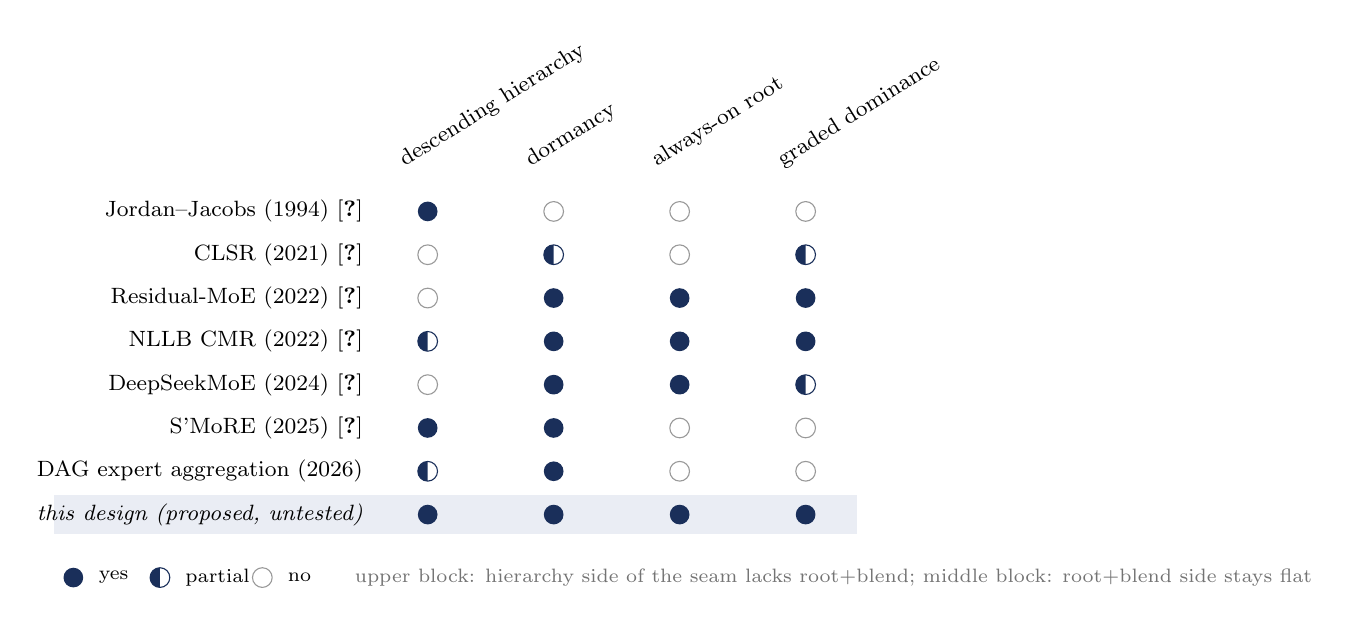
\begin{tikzpicture}[font=\small]
% dot macros: yes / partial / no
\def\Y#1#2{\fill[navy] (#1,#2) circle (0.125);}
\def\N#1#2{\draw[black!40] (#1,#2) circle (0.125);}
\def\P#1#2{\draw[navy] (#1,#2) circle (0.125);
  \fill[navy] (#1,#2) ++(90:0.125) arc (90:270:0.125);}
% highlight row for the proposed design
\fill[accent!10] (-4.6,-4.10) rectangle (5.6,-3.60);
% column headers
\node[rotate=32, anchor=south west, font=\footnotesize] at (-0.15,0.35) {descending hierarchy};
\node[rotate=32, anchor=south west, font=\footnotesize] at (1.45,0.35) {dormancy};
\node[rotate=32, anchor=south west, font=\footnotesize] at (3.05,0.35) {always-on root};
\node[rotate=32, anchor=south west, font=\footnotesize] at (4.65,0.35) {graded dominance};
% row labels
\node[anchor=east, font=\footnotesize] at (-0.55,0)     {Jordan--Jacobs (1994)~\cite{jordan1994}};
\node[anchor=east, font=\footnotesize] at (-0.55,-0.55) {CLSR (2021)~\cite{zhang2021clsr}};
\node[anchor=east, font=\footnotesize] at (-0.55,-1.10) {Residual-MoE (2022)~\cite{rajbhandari2022}};
\node[anchor=east, font=\footnotesize] at (-0.55,-1.65) {NLLB CMR (2022)~\cite{nllb2022}};
\node[anchor=east, font=\footnotesize] at (-0.55,-2.20) {DeepSeekMoE (2024)~\cite{dai2024}};
\node[anchor=east, font=\footnotesize] at (-0.55,-2.75) {S'MoRE (2025)~\cite{smore2025}};
\node[anchor=east, font=\footnotesize] at (-0.55,-3.30) {DAG expert aggregation (2026)};
\node[anchor=east, font=\footnotesize\itshape] at (-0.55,-3.85) {this design (proposed, untested)};
% dots: columns at x = 0.15, 1.75, 3.35, 4.95
\Y{0.15}{0}     \N{1.75}{0}     \N{3.35}{0}     \N{4.95}{0}
\N{0.15}{-0.55} \P{1.75}{-0.55} \N{3.35}{-0.55} \P{4.95}{-0.55}
\N{0.15}{-1.10} \Y{1.75}{-1.10} \Y{3.35}{-1.10} \Y{4.95}{-1.10}
\P{0.15}{-1.65} \Y{1.75}{-1.65} \Y{3.35}{-1.65} \Y{4.95}{-1.65}
\N{0.15}{-2.20} \Y{1.75}{-2.20} \Y{3.35}{-2.20} \P{4.95}{-2.20}
\Y{0.15}{-2.75} \Y{1.75}{-2.75} \N{3.35}{-2.75} \N{4.95}{-2.75}
\P{0.15}{-3.30} \Y{1.75}{-3.30} \N{3.35}{-3.30} \N{4.95}{-3.30}
\Y{0.15}{-3.85} \Y{1.75}{-3.85} \Y{3.35}{-3.85} \Y{4.95}{-3.85}
% legend
\Y{-4.35}{-4.65} \node[anchor=west, font=\scriptsize] at (-4.15,-4.65) {yes};
\P{-3.25}{-4.65} \node[anchor=west, font=\scriptsize] at (-3.05,-4.65) {partial};
\N{-1.95}{-4.65} \node[anchor=west, font=\scriptsize] at (-1.75,-4.65) {no};
\node[anchor=west, font=\scriptsize, text=black!55] at (-0.9,-4.65)
  {upper block: hierarchy side of the seam lacks root+blend; middle block: root+blend side stays flat};
\end{tikzpicture}
\caption{The D1 seam as a property scorecard. No published system fills all
four columns: works with a genuine descending expert hierarchy (S'MoRE, DAG
aggregation, Jordan--Jacobs) lack the always-on root and the graded blend,
while works with an always-on root and a learned graded blend (NLLB CMR,
Residual-MoE) keep their specialists flat. Verdicts follow the
source-verified audit scorecards; the final row is this paper's proposal,
which was never executed at scale (Section~\ref{sec:experiments}).}
\label{fig:seam}
\end{figure}

\begin{figure}[htbp]
\centering
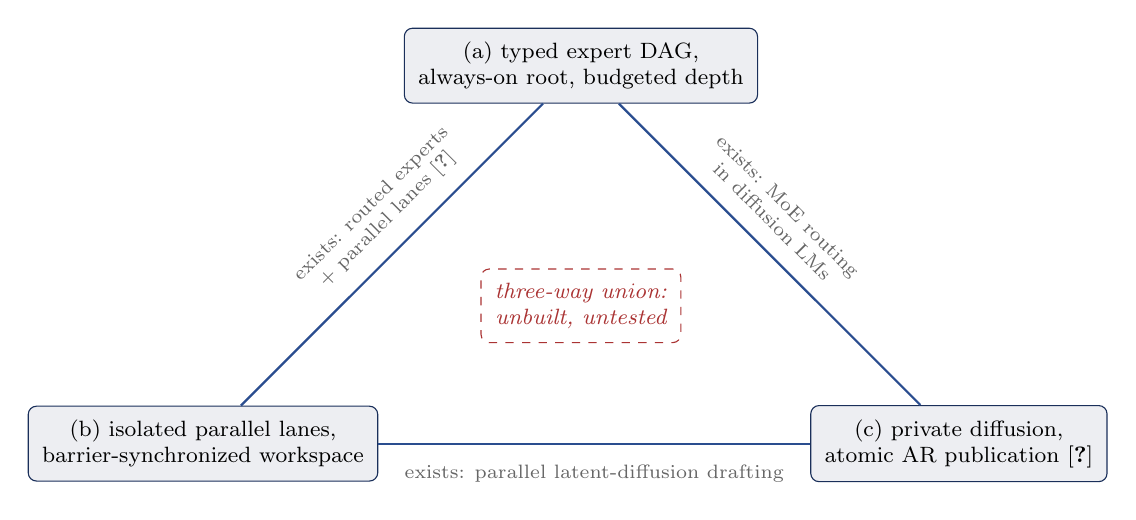
\begin{tikzpicture}[
  font=\small,
  pillar/.style={draw=navy, fill=navy!8, rounded corners=3pt, align=center,
    inner sep=5pt, font=\footnotesize},
  pairlabel/.style={font=\scriptsize, text=black!60, align=center},
  centernode/.style={draw=failred, dashed, rounded corners=3pt, align=center,
    inner sep=5pt, font=\footnotesize\itshape, text=failred}
]
\node[pillar] (A) at (0,3.4)     {(a) typed expert DAG,\\always-on root, budgeted depth};
\node[pillar] (B) at (-4.8,-1.4) {(b) isolated parallel lanes,\\barrier-synchronized workspace};
\node[pillar] (C) at (4.8,-1.4)  {(c) private diffusion,\\atomic AR publication~\cite{tidar2025}};
\draw[thick, accent] (A) -- (B) node[pairlabel, pos=0.45, sloped, above=3pt]
  {exists: routed experts\\+ parallel lanes~\cite{mot2025}};
\draw[thick, accent] (B) -- (C) node[pairlabel, midway, below=4pt]
  {exists: parallel latent-diffusion drafting};
\draw[thick, accent] (A) -- (C) node[pairlabel, pos=0.45, sloped, above=3pt]
  {exists: MoE routing\\in diffusion LMs};
\node[centernode] at (0,0.35) {three-way union:\\unbuilt, untested};
\end{tikzpicture}
\caption{The combination claim. Each pillar exists, and every pairwise
combination exists in a published system; only the three-way union in one
natively trained model was not found. The audit rates this bare union as a
design position, not a contribution, since no experiment shows the union
outperforming its best pairwise baseline.}
\label{fig:pillars}
\end{figure}

\begin{figure}[htbp]
\centering
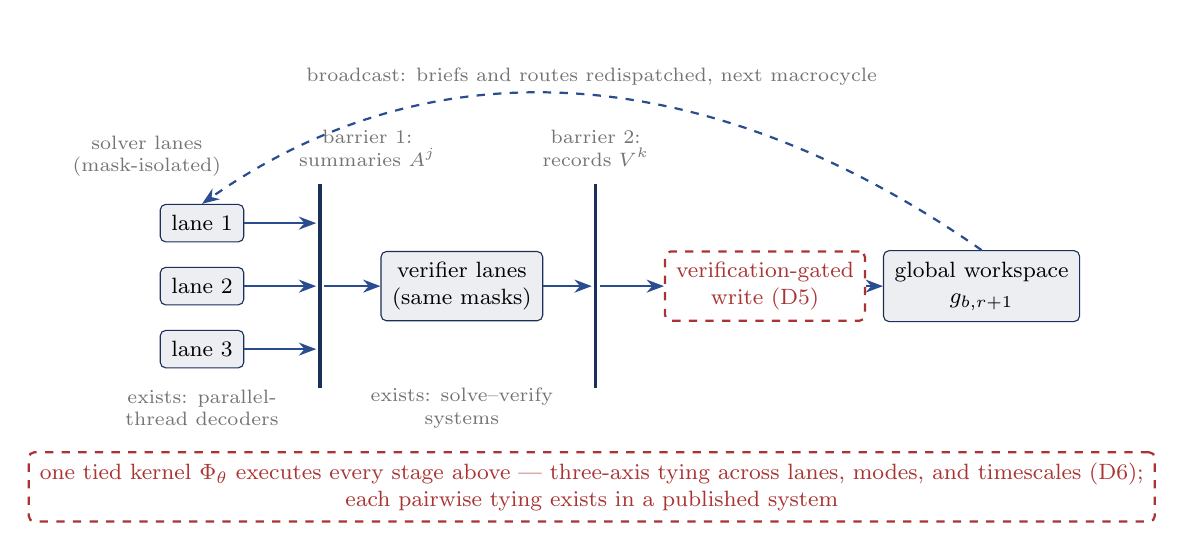
\begin{tikzpicture}[
  font=\footnotesize,
  known/.style={draw=navy, fill=navy!8, rounded corners=2pt, align=center,
    inner sep=4pt, font=\footnotesize},
  delta/.style={draw=failred, dashed, thick, rounded corners=2pt,
    align=center, inner sep=4pt, font=\footnotesize, text=failred},
  note/.style={font=\scriptsize, text=black!55, align=center},
  flow/.style={-{Stealth[length=2.2mm]}, thick, accent}
]
% solver lanes
\node[known] (l1) at (-6.0,1.0)  {lane 1};
\node[known] (l2) at (-6.0,0.2)  {lane 2};
\node[known] (l3) at (-6.0,-0.6) {lane 3};
\node[note] at (-6.7,1.85) {solver lanes\\(mask-isolated)};
\node[note] at (-6.0,-1.35) {exists: parallel-\\thread decoders};
% barrier 1
\draw[very thick, navy] (-4.5,-1.1) -- (-4.5,1.5);
\node[note] at (-3.9,1.95) {barrier 1:\\summaries $A^j$};
% verifiers
\node[known] (ver) at (-2.7,0.2) {verifier lanes\\(same masks)};
\node[note] at (-2.7,-1.35) {exists: solve--verify\\systems};
% barrier 2
\draw[very thick, navy] (-1.0,-1.1) -- (-1.0,1.5);
\node[note] at (-1.0,1.95) {barrier 2:\\records $V^k$};
% gated write (delta)
\node[delta] (gate) at (1.15,0.2) {verification-gated\\write (D5)};
% workspace
\node[known] (gw) at (3.9,0.2) {global workspace\\$g_{b,r+1}$};
% flows
\draw[flow] (l1.east) -- (-4.55,1.0);
\draw[flow] (l2.east) -- (-4.55,0.2);
\draw[flow] (l3.east) -- (-4.55,-0.6);
\draw[flow] (-4.45,0.2) -- (ver.west);
\draw[flow] (ver.east) -- (-1.05,0.2);
\draw[flow] (-0.95,0.2) -- (gate.west);
\draw[flow] (gate.east) -- (gw.west);
\draw[flow, dashed] (gw.north) to[out=145,in=35]
  node[note, above, pos=0.5] {broadcast: briefs and routes redispatched, next macrocycle}
  (l1.north);
% tied kernel (delta)
\node[delta, minimum width=11.6cm] at (-1.05,-2.35)
  {one tied kernel $\Phi_\theta$ executes every stage above ---
   three-axis tying across lanes, modes, and timescales (D6);\\
   each pairwise tying exists in a published system};
\end{tikzpicture}
\caption{The parallel-workspace pillar under the audit. Solid navy components
are anticipated: mask-isolated parallel lanes with fork--join summaries, and
native solve-then-verify stages, each exist in published systems. Dashed red
components are residual deltas: using structured verification records as the
gating input to the workspace write (D5), and tying one transition kernel
simultaneously across lanes, functional modes, and timescales (D6). Neither
delta carries empirical support; the workspace channel of this program
reached parity, not improvement (Section~\ref{sec:experiments}).}
\label{fig:workspace-audit}
\end{figure}

\begin{figure}[htbp]
\centering
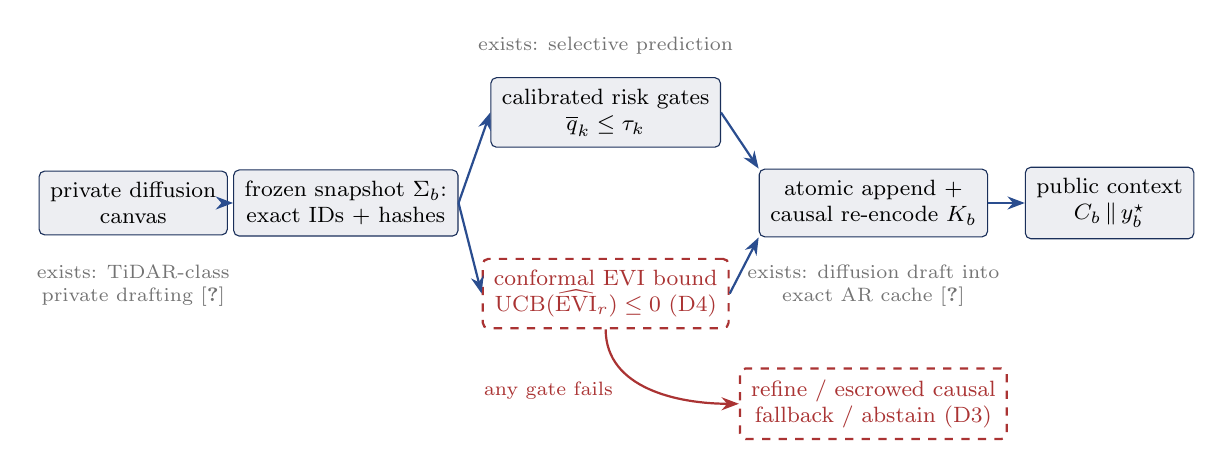
\begin{tikzpicture}[
  font=\footnotesize,
  known/.style={draw=navy, fill=navy!8, rounded corners=2pt, align=center,
    inner sep=4pt, font=\footnotesize},
  delta/.style={draw=failred, dashed, thick, rounded corners=2pt,
    align=center, inner sep=4pt, font=\footnotesize, text=failred},
  note/.style={font=\scriptsize, text=black!55, align=center},
  flow/.style={-{Stealth[length=2.2mm]}, thick, accent}
]
\node[known] (canvas) at (-6.7,0) {private diffusion\\canvas};
\node[note] at (-6.7,-1.05) {exists: TiDAR-class\\private drafting~\cite{tidar2025}};
\node[known] (snap) at (-4.0,0) {frozen snapshot $\Sigma_b$:\\exact IDs + hashes};
\node[known] (risk) at (-0.7,1.15) {calibrated risk gates\\$\overline{q}_k \le \tau_k$};
\node[note] at (-0.7,2.0) {exists: selective prediction};
\node[delta] (evi) at (-0.7,-1.15) {conformal EVI bound\\$\op{UCB}(\widehat{\op{EVI}}_r) \le 0$ (D4)};
\node[known] (commit) at (2.7,0) {atomic append +\\causal re-encode $K_b$};
\node[note] at (2.7,-1.05) {exists: diffusion draft into\\exact AR cache~\cite{tidar2025}};
\node[known] (pub) at (5.7,0) {public context\\$C_b \,\|\, y^\star_b$};
\node[delta] (fb) at (2.7,-2.55) {refine / escrowed causal\\fallback / abstain (D3)};
\draw[flow] (canvas.east) -- (snap.west);
\draw[flow] (snap.east) -- (risk.west);
\draw[flow] (snap.east) -- (evi.west);
\draw[flow] (risk.east) -- (commit.north west);
\draw[flow] (evi.east) -- (commit.south west);
\draw[flow] (commit.east) -- (pub.west);
\draw[flow, failred] (evi.south) to[out=-90,in=180]
  node[note, below left, pos=0.3, text=failred] {any gate fails}
  (fb.west);
\end{tikzpicture}
\caption{The private-to-public publication channel under the audit. Solid
navy components are anticipated: private non-autoregressive drafting behind
an exact autoregressive cache is solved by TiDAR~\cite{tidar2025}, and
calibrated per-failure-mode risk gating is standard selective prediction.
Dashed red components are residual deltas: the episode-level conformal bound
on compute-priced continuation value, valid under repeated adaptive
inspection (D4), and the ledger-escrowed fallback path that a failed gate
cannot bypass (D3). Both are untested constructions.}
\label{fig:pubchannel}
\end{figure}

\emph{In plain terms:} what remains unbuilt is (D1--D2) an expert layer
organized like a staffing tree, where a generalist always speaks first,
specialists are consulted only down the relevant branch, their evidence is
passed back up, and a learned dial sets how loudly the specialists speak
relative to the generalist; (D3) a budget office that will not let the model
start work it cannot afford to check and publish; (D4) a statistically
calibrated rule for deciding whether one more attempt is worth its compute
price; (D5) a shared whiteboard that only fact-checked notes may update;
(D6) one engine reused for every role instead of separate machinery per
role; and (D7) a training-time guarantee that the generalist provably stays
competent while specialists are added.

\subsection{Evidence on performance}

To be unambiguous about what the record does and does not contain: this
program produced \emph{no evidence that any of the residual deltas improves
model performance}. The experiments of Section~\ref{sec:experiments} retired
the mechanisms that were built. The strongest positive internal results are
of two kinds. First, calibrated selective prediction --- the one component
that repeatedly passed its preregistered gates --- worked reliably, but it is
an anticipated mechanism, not a residual delta. Second, the repaired
workspace channel of Experiment~9 reached \emph{parity} with causal
decoding, and the expert-graph removal in the reduction study cost roughly a
quarter of probe content accuracy while the graph was failing every causal
gate: the experts demonstrably carried content without demonstrably causing
better answers. Parity and stranded capacity are not improvements.

The positive performance evidence that exists attaches to the anticipated
\emph{ingredients}, in other people's systems, as reported by their authors
and not re-verified here: Residual-MoE reports quality on par with
substantially larger standard MoE models~\cite{rajbhandari2022};
Mixture-of-Recursions reports matched or improved quality at equal training
compute with higher inference throughput~\cite{mor2025}; conditional MoE
routing was adopted in the production-scale NLLB-200 system~\cite{nllb2022};
CLSR reports multilingual translation gains while allocating only 10--30\%
of routed computation to language-specific capacity~\cite{zhang2021clsr};
and TiDAR reports autoregressive-level quality at substantially higher
decoding throughput~\cite{tidar2025}. This is precisely the asymmetry the
audit exposes: the ingredients have performance evidence, the seven
assemblies have none, and no experiment anywhere --- including here --- has
yet tested whether any assembly outperforms its best flat or pairwise
baseline.

\subsection{Interpretation}

Novelty and validation are separate axes. Every item above is novel in the
narrow sense that no prior instantiation was found under adversarial search;
none is validated, and this paper's own experiments retire the program that
proposed them. The audit rated each surviving delta as, at most, material
for a related-work distinction. D1 is the best characterized: it is a named
seam between two developed lineages, with a minimal decisive experiment
available --- hold NLLB's CMR blend fixed and replace the flat expert pool
with a hierarchy that routing descends --- which is far smaller than the
program this paper reports.

% ================================================================ 13
\section{Conclusion}
\label{sec:conclusion}

This paper asked whether a hierarchical latent workspace, comprising a
root-preserving expert graph, isolated parallel lanes refined by categorical
diffusion, and calibrated atomic publication, improves verified answer
quality on a small frozen substrate at matched compute. Ten preregistered
experiments return a clear answer: not in the proposed form. The value of
the record is that every negative is mechanistic rather than bare. Each
mechanism failed in a specific, diagnosable, and ultimately reproducible
way, each diagnosis forced an instrument correction that survivors of this
design space will need, and the one component that repeatedly worked,
calibrated selective prediction, is exactly the component whose training
signal made it necessary.

Ten preregistered experiments on a 0.6B frozen substrate have answered the
question they were built to answer, mostly by removing possibilities. The
substrate hosted the dual-mode workspace stably in every experiment, with zero
skipped optimizer updates at every scale attempted. The evaluation stack is
honest: graders are semantic, abstention is a publishable answer, thresholds
are fitted on generated held-out emissions, audits reload checkpoints in
fresh processes, and every gate is declared before the run. All three
proposed mechanisms have now been retired by that machinery.

The routing mechanism, the part that decides \emph{which expertise to apply},
failed first. A marginal-entropy regularizer was found to make routing
probabilities uniform while leaving decisions concentrated, homogenizing the
experts it was meant to diversify; replacing it with hard-assignment load
balancing produced, on one seed, the first routing in the program to clear the
preregistered load gates, while the sibling seed collapsed entirely. With
both preregistered variance fixes applied and everything else frozen, the
collapsing seed collapsed again, the passing seed's diversity decayed to the
gate line, and the causal-liveness gate failed on ten of ten seed-runs. The
reduction rule then ran the design at two experts, the same seed collapsed a
third time, and the expert graph left the small-scale claim, at a measured
cost of roughly a quarter of probe content accuracy, which showed the experts
had been carrying content while failing every causal gate.

The verified-fan-in mechanism failed second, and its failure had two layers.
Experiment 8's selector was near-oracle and still lost by thirty points, because a
single mis-specified token identifier had knocked the workspace generation
channel into the wrong register, and Experiment 8's headline was arithmetically
unwinnable besides, with two to four points of selection headroom at its
operating accuracy. Experiment 9 repaired both: the channel reached parity with
causal decoding, zero scaffold leaks in 640 rows, and the comparison moved to
the difficulty stratum where selection could in principle matter. The stratum
proved empty, no exactly-one-correct rows on either seed, and the weighting
flipped two votes in 640 rows. Selection at this scale is void for headroom
on honest data, and demonstrating it will require rows this program's anchor
distribution does not contain.

The latent workspace itself, the architecture's central object, failed last
and most cleanly. With the register defect repaired, the finding is bounded
twice: ablating the read-out's memory positions changed graded accuracy by
0.000 on one seed and improved it by 0.022 on the other, and the causal arm,
which is the workspace arm with the whole prefix removed, sat within 0.013 of
it on both seeds. A post-session code audit added the structural half of the
diagnosis: the frozen decoder's input normalization makes the visible prefix
content independent of the learned gate, and the fluency anchor's reference
is the same model without the prefix, so the training design's only stable
point was a prefix that changes nothing. The latent workspace at
this scale is not damaged, expensive, or unstable; it is unnecessary, and the
model behaves accordingly. The mechanism-level lesson generalizes beyond this
architecture: a bolted-on reasoning structure whose information is redundant
with the decoder's own input will be ignored by a sufficiently capable
decoder, and no amount of interface repair changes that.

Experiment 10 then removed the redundancy and asked again. With the premise
physically withheld from the answer path, training conducted under that same
asymmetry, and an instrument that was airtight on its own gates, zero leaks,
an exact 0.000 causal floor, a trained attribution control at 0.000, and
parity preserved on unmasked rows, masked accuracy still read 0.000 on both
seeds while a linear probe recovered roughly a third of the withheld premise
from the latent state. Necessity, the constraint Experiment 9 bequeathed, is
therefore necessary but not sufficient: making the latent the only source
makes its failure measurable, and it fails. What ten experiments never gave the
latent is a dense token-level objective through the latent itself, the one
ingredient shared by the published systems that do pass content through
learned latent tokens~\cite{codi2025,coconut2024}, whose ablations reproduce
this program's probe-positive, generation-zero signature exactly. That is
the successor's hypothesis, preregistered elsewhere, and not this paper's
claim.

The calibrated-commitment half of the architecture survived longest, and its
trajectory is the most instructive. The split-conformal publication rule
delivered controlled coverage where six earlier runs had produced degenerate
thresholds and Experiment 8 had strangled at 0.078; its operating points were
flawless in Experiment 9, 138 published answers and 138 correct, and again in
Experiment 10, 160 published and 158 correct with risk upper bounds at 0.072 and
0.038; it lost its risk--coverage comparison to matched mean-log-probability
abstention on both Experiment 9 seeds, and then beat that baseline directionally
on both Experiment 10 seeds, at paired-bootstrap win fractions of 0.746 and 0.792
against the preregistered 0.80 bar. The program's rules do not permit
renaming a near-miss a victory, so calibrated selective prediction at small
scale closes as unestablished, with a recorded effect direction, an effect
size, and the power analysis a successor needs: at 288 audit rows per seed
the design could only detect an effect roughly three times the one observed.
The machinery works, replicates, and is one adequately powered audit away
from an answer either way.

The program therefore ends where its rules put it, and that is the result.
Zero of three mechanisms survive their own preregistered tests; the
decisive plain-LoRA control was never authorized and remains unrun, so no
capability claim of any kind is made; the scale-up candidate remains blocked
behind its data audit. What ten experiments support is a method and a record:
gates declared before every run, killer baselines inside every audit, failure
modes with named detectors, mechanisms retired on schedule rather than
rescued by narrative, and a taxonomy of the specific ways a
latent-workspace architecture fails at small scale, each with a detector,
each measured, several repaired, none rescued. A reader building in this
space inherits the constraint that matters, now in its final form: do not ask
whether the model uses your mechanism when it does not have to; arrange the
world so it has to, and measure that; and when it still does not, supervise
the mechanism directly, because ten experiments of arranging the world were not
enough to make loss discover it.

% ================================================================ refs
\begin{thebibliography}{22}
\footnotesize
\setlength{\itemsep}{0.15em}

\bibitem{louizos2018}
C.~Louizos, M.~Welling, and D.~P. Kingma.
Learning sparse neural networks through $L_0$ regularization.
\emph{International Conference on Learning Representations}, 2018.
arXiv:1712.01312.

\bibitem{codi2025}
Z.~Shen, H.~Yan, L.~Zhang, Z.~Hu, Y.~Du, and Y.~He.
CODI: Compressing chain-of-thought into continuous space via self-distillation.
\emph{Empirical Methods in Natural Language Processing}, 2025.
arXiv:2502.21074.

\bibitem{coconut2024}
S.~Hao, S.~Sukhbaatar, D.~Su, X.~Li, Z.~Hu, J.~Weston, and Y.~Tian.
Training large language models to reason in a continuous latent space.
\emph{Conference on Language Modeling}, 2025.
arXiv:2412.06769.

\bibitem{diffusiongemma}
DiffusionGemma Team et~al.
DiffusionGemma technical report.
arXiv:2608.00146, 2026.

\bibitem{austin2021}
J.~Austin et~al.
Structured denoising diffusion models in discrete state-spaces.
\emph{Advances in Neural Information Processing Systems}, 2021.
arXiv:2107.03006.

\bibitem{chen2022}
T.~Chen, R.~Zhang, and G.~Hinton.
Analog bits: Generating discrete data using diffusion models with
self-conditioning.
arXiv:2208.04202, 2022.

\bibitem{nie2025}
S.~Nie et~al.
Large language diffusion models.
arXiv:2502.09992, 2025.

\bibitem{arriola2025}
M.~Arriola et~al.
Block diffusion: Interpolating between autoregressive and diffusion language
models.
arXiv:2503.09573, 2025.

\bibitem{shing2025}
M.~Shing, M.~Koyama, and T.~Akiba.
DiffusionBlocks: Block-wise neural network training via diffusion
interpretation.
arXiv:2506.14202v4, 2025.

\bibitem{benhamu2025}
H.~Ben-Hamu et~al.
Accelerated sampling from masked diffusion models via entropy bounded
unmasking.
arXiv:2505.24857, 2025.

\bibitem{lepikhin2021}
D.~Lepikhin et~al.
GShard: Scaling giant models with conditional computation and automatic
sharding.
\emph{International Conference on Learning Representations}, 2021.
arXiv:2006.16668.

\bibitem{fedus2022}
W.~Fedus, B.~Zoph, and N.~Shazeer.
Switch transformers: Scaling to trillion parameter models with simple and
efficient sparsity.
\emph{Journal of Machine Learning Research}, 23(120):1--39, 2022.
arXiv:2101.03961.

\bibitem{graves2016}
A.~Graves.
Adaptive computation time for recurrent neural networks.
arXiv:1603.08983, 2016.

\bibitem{dehghani2019}
M.~Dehghani, S.~Gouws, O.~Vinyals, J.~Uszkoreit, and {\L}.~Kaiser.
Universal transformers.
\emph{International Conference on Learning Representations}, 2019.
arXiv:1807.03819.

\bibitem{jordan1994}
M.~I. Jordan and R.~A. Jacobs.
Hierarchical mixtures of experts and the EM algorithm.
\emph{Neural Computation}, 6(2):181--214, 1994.

\bibitem{shazeer2017}
N.~Shazeer et~al.
Outrageously large neural networks: The sparsely-gated mixture-of-experts
layer.
\emph{International Conference on Learning Representations}, 2017.
arXiv:1701.06538.

\bibitem{dai2024}
D.~Dai et~al.
DeepSeekMoE: Towards ultimate expert specialization in mixture-of-experts
language models.
arXiv:2401.06066, 2024.

\bibitem{yao2023}
S.~Yao et~al.
Tree of Thoughts: Deliberate problem solving with large language models.
\emph{Advances in Neural Information Processing Systems}, 2023.
arXiv:2305.10601.

\bibitem{wang2023}
X.~Wang et~al.
Self-consistency improves chain of thought reasoning in language models.
\emph{International Conference on Learning Representations}, 2023.
arXiv:2203.11171.

\bibitem{hao2024}
S.~Hao et~al.
Training large language models to reason in a continuous latent space.
arXiv:2412.06769, 2024.

\bibitem{raposo2024}
D.~Raposo et~al.
Mixture-of-Depths: Dynamically allocating compute in transformer-based
language models.
arXiv:2404.02258, 2024.

\bibitem{cobbe2021}
K.~Cobbe et~al.
Training verifiers to solve math word problems.
arXiv:2110.14168, 2021.

\bibitem{kadavath2022}
S.~Kadavath et~al.
Language models (mostly) know what they know.
arXiv:2207.05221, 2022.

\bibitem{guo2017}
C.~Guo, G.~Pleiss, Y.~Sun, and K.~Q. Weinberger.
On calibration of modern neural networks.
\emph{International Conference on Machine Learning}, 2017.
arXiv:1706.04599.

\bibitem{rajbhandari2022}
S.~Rajbhandari, C.~Li, Z.~Yao, M.~Zhang, R.~Y. Aminabadi, A.~A. Awan,
J.~Rasley, and Y.~He.
DeepSpeed-MoE: Advancing mixture-of-experts inference and training to power
next-generation AI scale.
\emph{International Conference on Machine Learning}, 2022.
arXiv:2201.05596. Residual-MoE blend verified in the released
\texttt{deepspeed/moe/layer.py}.

\bibitem{zhang2021clsr}
B.~Zhang, A.~Bapna, R.~Sennrich, and O.~Firat.
Share or not? Learning to schedule language-specific capacity for
multilingual translation.
\emph{International Conference on Learning Representations}, 2021.

\bibitem{nllb2022}
NLLB Team, M.~R. Costa-juss\`a, et~al.
No language left behind: Scaling human-centered machine translation.
arXiv:2207.04672, 2022. Conditional MoE Routing, \S8.

\bibitem{smore2025}
Structural mixture of residual experts (S'MoRE).
arXiv:2504.06426, 2025.

\bibitem{mor2025}
Mixture-of-Recursions: Learning dynamic recursive depths for adaptive
token-level computation.
arXiv:2507.10524, 2025.

\bibitem{mot2025}
Mixture of Thoughts.
arXiv:2509.21164, 2025.

\bibitem{tidar2025}
TiDAR: Think in diffusion, talk in autoregression.
arXiv:2511.08923, 2025.

\bibitem{hilp2026}
C.~Shi, T.~Pearce, M.~Tomar, S.~Sen, and J.~Langford.
Hierarchical latent prediction for language models.
arXiv:2608.05806, 2026.

\bibitem{da2026}
N.~Ho et~al.
Language models can control their own attention.
arXiv:2609.02737, 2026.

\bibitem{workspace2026}
W.~Gurnee, N.~Sofroniew, et~al.
Verbalizable representations form a global workspace in language models.
Transformer Circuits Thread, 2026.

\end{thebibliography}

\appendix
\section{Artifact Provenance and Reproducibility}
\label{app:provenance}

Every experiment in Section~\ref{sec:experiments} maps to an internal artifact
tag that identifies its preregistered plan, training checkpoints, and audit
records in the project repository. The tags are reproduced here so that
any reported number can be traced to its on-disk provenance.

\begin{table}[htbp]
\caption{Experiment-to-artifact provenance. Tags identify checkpoints, plans, and
audit records in the project repository.}
\label{tab:provenance}
\centering\small
\begin{tabularx}{\textwidth}{@{}llX@{}}
\toprule
\textbf{Experiment} & \textbf{Artifact tag} & \textbf{Question} \\
\midrule
Structural diagnostic & \studytag{legacy-cpu} & Do the code paths execute at all? (41k-parameter CPU network; verifies plumbing only.) \\
Experiment 1: Substrate transplant & \studytag{v5.2} & Can the frozen Qwen3-0.6B substrate host the dual-mode workspace stably? \\
Experiment 2: Graded evaluation & \studytag{v5.3} & Do semantic graders, safe-abstention publication, and threshold fitting produce honest measurements? \\
Experiment 3: Publication boundary & \studytag{v5.4} & Does fixing the publication boundary transfer calibration to generated candidates? \\
Experiment 4: On-policy calibration \& replication & \studytag{v5.5} & Do on-policy policy heads separate the model's own emissions, and does routing survive preregistered causal gates across independent seeds? \\
Experiment 5: Routing redesign on verified data & \studytag{v5.6} & Does hard-assignment load balancing produce causally live multi-expert routing, on execution-verified multi-domain data, across independent seeds? \\
Experiment 6: Targeted variance fixes & \studytag{v5.6.1} & Do nonzero expert initialization and family-balanced head-phase data rescue the collapse mode and lift commit accuracy on the same two seeds, everything else frozen? \\
Experiment 7: The reduction experiment & \studytag{v5.6.2} & At minimum viable expert count (two), does routing become reliable and causally live, with the same seeds, a validity-gated head phase, a generation-time canary and everything else frozen? \\
Experiment 8: Verified fan-in & \studytag{v6.0} & With the read-out bottleneck opened and the calibrated heads promoted from gate to selector, does the latent workspace beat self-consistency and logit-based selection at a matched candidate budget? \\
Experiment 9: Repaired channel, decoupled claims & \studytag{v8.0} & With the workspace channel's register defect repaired, does the channel reach causal parity, and do the calibrated heads out-select and out-abstain their free baselines on the \emph{same} healthy candidate pool? \\
Experiment 10: The necessary channel & \studytag{v9.0} & With the premise physically withheld from the causal path, so that ignoring the latent costs loss, does the workspace carry structurally necessary information into generation? \\
\bottomrule
\end{tabularx}
\end{table}


\end{document}
